\documentclass[11pt]{article}
\usepackage[sc]{mathpazo} %Like Palatino with extensive math support
\usepackage{fullpage}
\usepackage[authoryear,round,sectionbib,sort]{natbib}   % omit 'round' option if you prefer square brackets
\let\cite\citep


\linespread{1.7}
\usepackage[utf8]{inputenc}
\usepackage{lineno}
\usepackage{titlesec}

\usepackage{graphicx,float}
% for setting up equations
\usepackage{amsmath}

\usepackage[T1]{fontenc}

\usepackage[dvipsnames]{xcolor}

\titleformat{\section}[block]{\Large\bfseries\filcenter}{\thesection}{1em}{}
\titleformat{\subsection}[block]{\Large\itshape\filcenter}{\thesubsection}{1em}{}
\titleformat{\subsubsection}[block]{\large\itshape}{\thesubsubsection}{1em}{}
\titleformat{\paragraph}[runin]{\itshape}{\theparagraph}{1em}{}[. ]\renewcommand{\refname}{Literature Cited}



\usepackage{xcolor}
\newcommand{\tom}[2]{{\color{red}{#1}}\footnote{\textit{\color{red}{#2}}}}
\newcommand{\jacob}[2]{{\color{blue}{#1}}\footnote{\textit{\color{blue}{#2}}}}
\newcommand{\josh}[2]{{\color{orange}{#1}}\footnote{\textit{\color{orange}{#2}}}}
%%%%%%%%%%%%%%%%%%%%%
% Line numbering
%%%%%%%%%%%%%%%%%%%%%
%
% Please use line numbering with your initial submission and
% subsequent revisions. After acceptance, please turn line numbering
% off by adding percent signs to the lines %\usepackage{lineno} and
% to %\linenumbers{} and %\modulolinenumbers[3] below.
\linenumbers
% To avoid line numbering being thrown off around math environments,
% the math environments have to be wrapped using
% \begin{linenomath*} and \end{linenomath*}
%
% (Thanks to Vltimil Krivan for pointing this out to us!)

\title{Increasing prevalence of plant-fungal symbiosis across two centuries of environmental change}

% This version of the LaTeX template was last updated on
% September 28, 2022.

%%%%%%%%%%%%%%%%%%%%%
% Authorship
%%%%%%%%%%%%%%%%%%%%%
% Please remove authorship information while your paper is under review,
% unless you wish to waive your anonymity under double-blind review. You
% will need to add this information back in to your final files after
% acceptance.

\author{Joshua C. Fowler$^{1,2\ast}$ \\
	Jacob Moutouama$^{1}$\\
	Tom E. X. Miller$^{1}$}
\date{}

\begin{document}
	
	\maketitle
	
	\noindent{} 1. Rice University, Department of BioSciences, Houston, Texas 77006;
	\noindent{} 2. University of Miami, Department of Biology, Miami, Florida;


	\noindent{} $\ast$ Corresponding author; e-mail: jcf221@miami.edu.
	
	\bigskip
	
	\textit{Manuscript elements}: Figure~1, figure~2, table~1, appendix~A (for print; including figure~A1, figure~A2, and table~A1), supplemental PDF. Figure~2 is to print in color.
	
	\bigskip
	
	\textit{Keywords}: .
	
	\bigskip
	
	\textit{Manuscript type}: Article. %Or note, natural history miscellany note, comment, reply, invited symposium, featured topic, or historical perspective.
	
	\bigskip
	
	\noindent{\footnotesize Prepared using the suggested \LaTeX{} template for \textit{Am.\ Nat.}}
	
	%\linenumbers{}
	%\modulolinenumbers[3]
	
	\newpage{}
	
	\section*{Abstract}
Species' distributions and abundances are shifting in response to climate change. 
Most species harbor microbial symbionts that have the potential to influence these responses.
Mutualistic microbial symbionts may provide resilience to environmental change by protecting their hosts from increasing stress. 
However, environmental change that disrupts these interactions may lead to declines in hosts or symbionts. 
Microbes preserved within herbarium specimens offer a unique opportunity to quantify changes in microbial symbiosis across broad temporal and spatial scales. 
We asked how the prevalence of seed-transmitted fungal symbionts of grasses (\emph{Epichloë} endophytes), which can protect hosts from abiotic stress, have changed over time in response to climate change, and how these changes vary across host species' ranges.
Specifically, we analyzed 2,346 herbarium specimens of three grass host species collected over the last two centuries (1824 -- 2019) for the presence or absence of endophyte symbiosis, and evaluated spatial and temporal trends in endophyte prevalence. 
We found that endophytes have increased in prevalence over the last two centuries from ca. 25\% prevalence to ca. 75\% prevalence, on average, across the three host species.
We also found that changes in prevalence were associated with observed \tom{changes in seasonal climate drivers}{Describe ``changes'' -- warming? drying?} corresponding to each host species' peak growing season. 
Our analysis performed favorably in an out-of-sample predictive test, however we identified XXX as suggesting the model fusion may be an important step moving forward.
\jacob{Our results provide novel evidence for a cryptic biological response to climate change that may contribute to the resilience of host-microbe symbiosis through context-dependent benefits that confer a fitness advantage to symbiotic hosts under environmental change.}{I like this and the abstract in general. I agree with Tom and I think we  have some space to add these details. Abstract : 300}
	
	\newpage{}
	
	\section*{Introduction}
	
	% The journal does not have numbered sections in the main portion of
	% articles. Please refrain from using section references (à la
	% section~\ref{section:CountingOwlEggs}), and refer to sections by name
	% (e.g. section ``Counting Owl Eggs'').
	
Understanding how biotic interactions are altered by global change is a major goal of basic and applied ecological research \cite{gilman2010framework,blois2013climate}.
Documented responses to environmental change, such as shifts in species' distributions \cite{aitken2008adaptation} and phenology \cite{piao2019plant}, are typically blind to concurrent changes in associated biotic interactions.
Empirically evaluating these biotic changes -- whether interacting species shift in tandem with their partners or not \cite{hillerislambers2013will} -- is crucial to predicting the reorganization of Earth's biodiversity under global change. 
Such evaluations have been limited because few datasets on species interactions extend over sufficiently long time scales of contemporary climate change \cite{poisot2021global}.

Natural history specimens, which were originally collected to study and preserve taxonomic diversity, present a unique opportunity to explore long-term changes in ecological interactions across broad spatial and temporal scales \citep{meineke2018unrealized}. 
Natural history collections, built and maintained by the efforts of thousands of scientists, are invaluable time machines, primarily comprised of physical specimens of organisms along with information about the time and place of their collection. 
These specimens often preserve physical legacies of ecological processes and species' interactions from dynamically changing environments across time and space.
For example, previous researchers have used plant collections (herbaria) to document shifts in phenology \citep{willis2017old, park2019herbarium,  berg2019examination}, pollination \citep{pauw2011reconstruction, duan2019century}, and herbivory \citep{meineke2019herbarium} related to anthropogenic climate change. 
However, few previous studies have leveraged biological collections to examine climate change-related shifts in a particularly common type of interaction: microbial symbiosis.

Microbial symbionts are common to all macroscopic organisms and can have important effects on their hosts' survival, growth and reproduction \cite{rodriguez2009fungal,mcfall2013animals}.
Many microbial symbionts act as mutualists, engaging in reciprocally beneficial interactions with their hosts that can ameliorate environmental stress. 
For example, bacterial symbionts of insects, such as \emph{Wolbachia}, can improve their hosts' thermal tolerance \citep{truitt2019wolbachia, renoz2019evolutionary}, and arbuscular mycorrhizal fungi, documented in 70-90\% of families of land plants \citep{parniske2008arbuscular}, allow their hosts to persist through drought conditions by improving water and nutrient uptake \citep{cheng2021elucidating}.
On the other hand, changes in the mean and variance of environmental conditions may disrupt microbial  mutualisms by changing the costs and benefits of the interaction for each partner, leading the interaction to deteriorate \citep{aslan2013mutualism, fowler2024microbial}. 
Coral bleaching (the loss of symbiotic algae) due to temperature stress \citep{sully2019global} is perhaps the best known example, but this phenomenon is not unique to corals.
Lichens exposed to elevated temperatures experienced loss of photosynthetic function along with changes in the composition of their algal symbiont community \citep{meyer2022climate}.
How commonly and under what conditions microbial mutualisms deteriorate or strengthen under climate change remain unanswered questions.
Previous work suggests that these alternative responses may depend on the intimacy and specialization of the interaction as well as the physiological tolerances of the mutualist partners \citep{toby2010mutualisms, warren2014mutualism, rafferty2015phenological}. 

Understanding of how microbial symbioses are affected by climate change is additionally complicated by spatial heterogeneity in the direction and magnitude of environmental change \cite{ipcc_2021}. 
Beneficial symbionts are likely able to shield their hosts from environmental stress in locations that experience a small degree of change, but symbionts in locations that experience changes of large magnitude may be pushed beyond their physiological limits \cite{webster2008temperature}.
Additionally, symbionts are often unevenly distributed across their hosts' distribution.
Facultative symbionts may be absent from portions of the host range \cite{afkhami2014mutualist}, and hosts may engage with a diversity of partners (different symbiont species or locally-adapted strains) across their environments \cite{frade2008variation, rolshausen2018quantifying}.
Identifying broader spatial trends in symbiont prevalence is therefore an important step in developing predictions for where to expect changes in the symbiosis in future climates.

\emph{Epichloë} fungal endophytes are specialized symbionts of cool-season grasses, which have been documented in $\sim 30$\% of cool-season grass species \citep{leuchtmann1992systematics}.
They are transmitted vertically from maternal plants to offspring through seeds.
Vertical transmission creates a feedback between the fitness of host and symbiont \citep{fine1975vectors, douglas1998host, rudgers2009fungus}. 
Over time, endophytes that act as mutualists should rise in prevalence within a host population \citep{donald2021context}. 
\emph{Epichloë} are known to improve their hosts' drought tolerance \cite{decunta2021systematic} and protect their hosts against herbivores \cite{crawford2010fungal} and pathogens \cite{xia2018role} likely through the production of a diverse suite of alkaloids and other secondary metabolites.
The fitness feedback induced by vertical transmission leads to the prediction that endophyte prevalence should be high in populations where these fitness benefits are most important. 
Previous contemporary survey studies have documented large-scale spatial patterns in  endophyte prevalence structured by environmental gradients \citep{granath2007variation,bazely2007broad, afkhami2012fungal,sneck2017variation}.
We predicted that prevalence should track temporal changes in environmental drivers that elicit these fitness benefits.
%For example, endophyte-mediated drought tolerance should lead endophyte prevalence to increase in regions where precipitation has declined over time.

Early research on \emph{Epichloë} used herbarium specimens to describe the broad taxonomic diversity of host species that harbor these symbionts \citep{white1985endophyte}, \josh{establishing that endophyte symbiosis could be identified in plant tissue from as early as 1851.}{Edited this a bit. This is the earliest year we have in the database that was part of JFWhites original paper.} 
However, no subsequent studies, to our knowledge, have used the vast resources of biological collections to quantitatively assess spatio-temporal trends in endophyte prevalence and their environmental correlates. 
Grasses are commonly collected and identified based on the presence of their reproductive structures, meaning that preserved specimens typically contain seeds, conveniently preserving the fungi along with their host plants on herbarium sheets. 
This creates the opportunity to leverage the unique spatio-temporal sampling of herbarium collections to examine the response of the symbiosis to historical climate change. 
\josh{Research using historical collections has clearly demonstrated other ecological signatures of a changing climate. 
However the predictive ability of these historical analyses is rarely tested against contemporary data \citep{lee2024phenological}. 
Identifying the ways in which these analyses fall short is a crucial step for the field move from reading signatures in the past to forecasting ecological dynamics into the future.}{what do you think of this? trying to presage the out-of-sample test without over promising and without saying outright that our analysis sucks. Is this the right place for this? I had imagined some of this material will be really developed in the discussion.}

In this study, we assessed the long-term responses of endophyte symbiosis to climate change through the use of herbarium specimens of three North American host grass species (\emph{Agrostis hyemalis}, \emph{Agrostis perennans}, and \emph{Elymus virginicus}).
We first address questions describing spatial and temporal trends in endophyte prevalence: (i) How has endophyte prevalence changed over the past two centuries? and (ii) How spatially variable are temporal trends in endophyte prevalence across eastern North America?
We then address how climate change may be driving trends in endophyte prevalence by asking: (iii) What is the relationship between variation in temporal trends in endophyte prevalence and changes in climate drivers?
We predicted that aggregate endophyte prevalence would increase over time in tandem with climate warming, and that hotspots of endophyte change would correspond spatially to hotspots of climate change. 
Finally, we evaluated the performance of models built on data from historic specimens with an out-of-sample test, data on endophyte prevalence from contemporary surveys of host populations. 
To answer these questions we examined a total of 2,346 specimens collected across eastern North America between 1824 and 2019.
\tom{}{I think the consensus was to keep the out-of-sample validation which should absolutely go into the Intro as an important element of novelty. Should go in the Asbtract too.}
	
\section*{Methods}
        \subsection*{Focal species}
Our surveys focused on three native North American grasses: \emph{Agrostis hyemalis}, \emph{Agrostis perennans}, and \emph{Elymus virginicus}. 
Both \emph{Agrostis} species host \emph{Epichloë amarillans} \cite{craven2001multigene, leuchtmann2014nomenclatural}, while \emph{Elymus virginicus} typically hosts \emph{Epichloë elymi} \cite{clay2002evolutionary}.
These $C_3$ grass species are commonly represented in natural history collections with broad distributions covering much the eastern United States.
\emph{A. hyemalis} is a small short-lived perennial species that germinates in the spring and typically flowers between March and July (most common collection month: May).
\emph{A. perennans} is of similar stature but is longer lived than \emph{Agrostis hyemalis} and flowers in late summer and early autumn (most common collection month: September). 
\emph{A. perennans} is more sparsely distributed, tending to be found in shadier and more moist habitats, while \emph{A. hyemalis} is commonly found in open and recently disturbed ground. 
Both \emph{Agrostis} species are recorded from throughout the Eastern US, but \emph{A. perennans} has a slightly more northern distribution, whereas \emph{A. hyemalis} is found rarely as far north as Canada and is listed as a rare plant in Minnesota.
\emph{E. virginicus} is a larger and relatively longer-lived  species that is more broadly distributed than the \emph{Agrostis} species. 
It begins flowering as early as March or April but continues throughout the summer (most common collection month: July).

		\subsection*{Herbarium surveys}
We visited nine herbaria between 2019 and 2022 (see Table A1 for a summary of specimens included from each collection). 
With permission from herbarium staff, we acquired seed samples from $1135$ \emph{A. hyemalis} specimens collected between 1824 and 2019, $357$ \emph{A. perennans} specimens collected between 1863 and 2017, and $854$ \emph{E. virginicus} specimens collected between 1839 and 2019 (Fig. \ref{fig:map}, Fig. \ref{fig:temporal}A, Fig. \ref{fig:endo_status_map}).
%Our sampling plan was designed to minimize damage to these specimens.
We chose our focal species in part because they are commonly represented in herbarium collections, and produce high numbers of seeds, meaning that small samples would not diminish the value of the specimens for future studies. 
We collected 5-10 seeds per specimen after examining the herbarium sheet under a dissecting microscope to ensure that we collected mature seeds, not florets or unfilled seeds, fit for our purpose of identifying fungal endophytes with microscopy.
We excluded specimens for which information about the collection location and date were unavailable.
Each specimen was assigned geographic coordinates based on collection information recorded on the herbarium sheet using the geocoding functionality of the ggmap R package \citep{kahle2019package}.
Many specimens had digitized collection information readily available, but for those that did not, we transcribed information printed on the herbarium sheet. 
Collections were geo-referenced to the nearest county centroid, or nearest municipality when that information was available. 
For a few of the oldest specimens, only information at the state level was available, and so we used the state centroid.


After collecting seed samples, we quantified the presence or absence of \emph{Epichloë} fungal hyphae, which grow intercellularly, in each specimen using microscopy. 
We first softened seeds with a 10\% NaOH solution, then stained the seeds with aniline blue-lactic acid stain and squashed them under a microscope cover slip. 
We examined the squashed seeds for the presence of fungal hyphae at 200-400X magnification \cite{bacon2018stains}.
In some cases, the tissues examined during microscopy came from flowers or otherwise non-viable seeds, which were excluded for that specimen.
On average we scored $4.7$ seeds per specimen of \emph{A. hyemalis}, $4.2$ seeds per specimen of \emph{A. perennans}, and $3.8$ seeds per specimen of \emph{E. virginicus}; we scored \# seeds in total. .
Due to imperfect vertical transmission \cite{afkhami2008symbiosis}, it is possible that symbiotic host-plants produce a mixture of symbiotic and non-symbiotic seeds. 
We therefore designated a specimen as endophyte-symbiotic if \emph{Epichloë} hyphae were observed in one or more of its seeds, or non-symbiotic if hyphae were observed in none of its seeds. 
To capture uncertainty in the endophyte scoring process, we recorded both a "liberal" and a "conservative" endophyte status for each plant specimen.  
When we identified potential endophytes with unusual morphology, low uptake of stain, or a small amount of fungal hyphae across the scored seeds, we recorded a positive liberal status (more likely to be endophyte-positive) and a negative conservative status (less likely to be endophyte-positive). 
$89$\% of scored plants had matching liberal and conservative scores, reflecting high confidence in endophyte status.
The following analyses in the main text used the liberal status, but we repeated all analyses with the conservative status which yielded qualitatively similar results (Fig. \ref{fig:FigA5})

\begin{figure}[h]
	\centering
	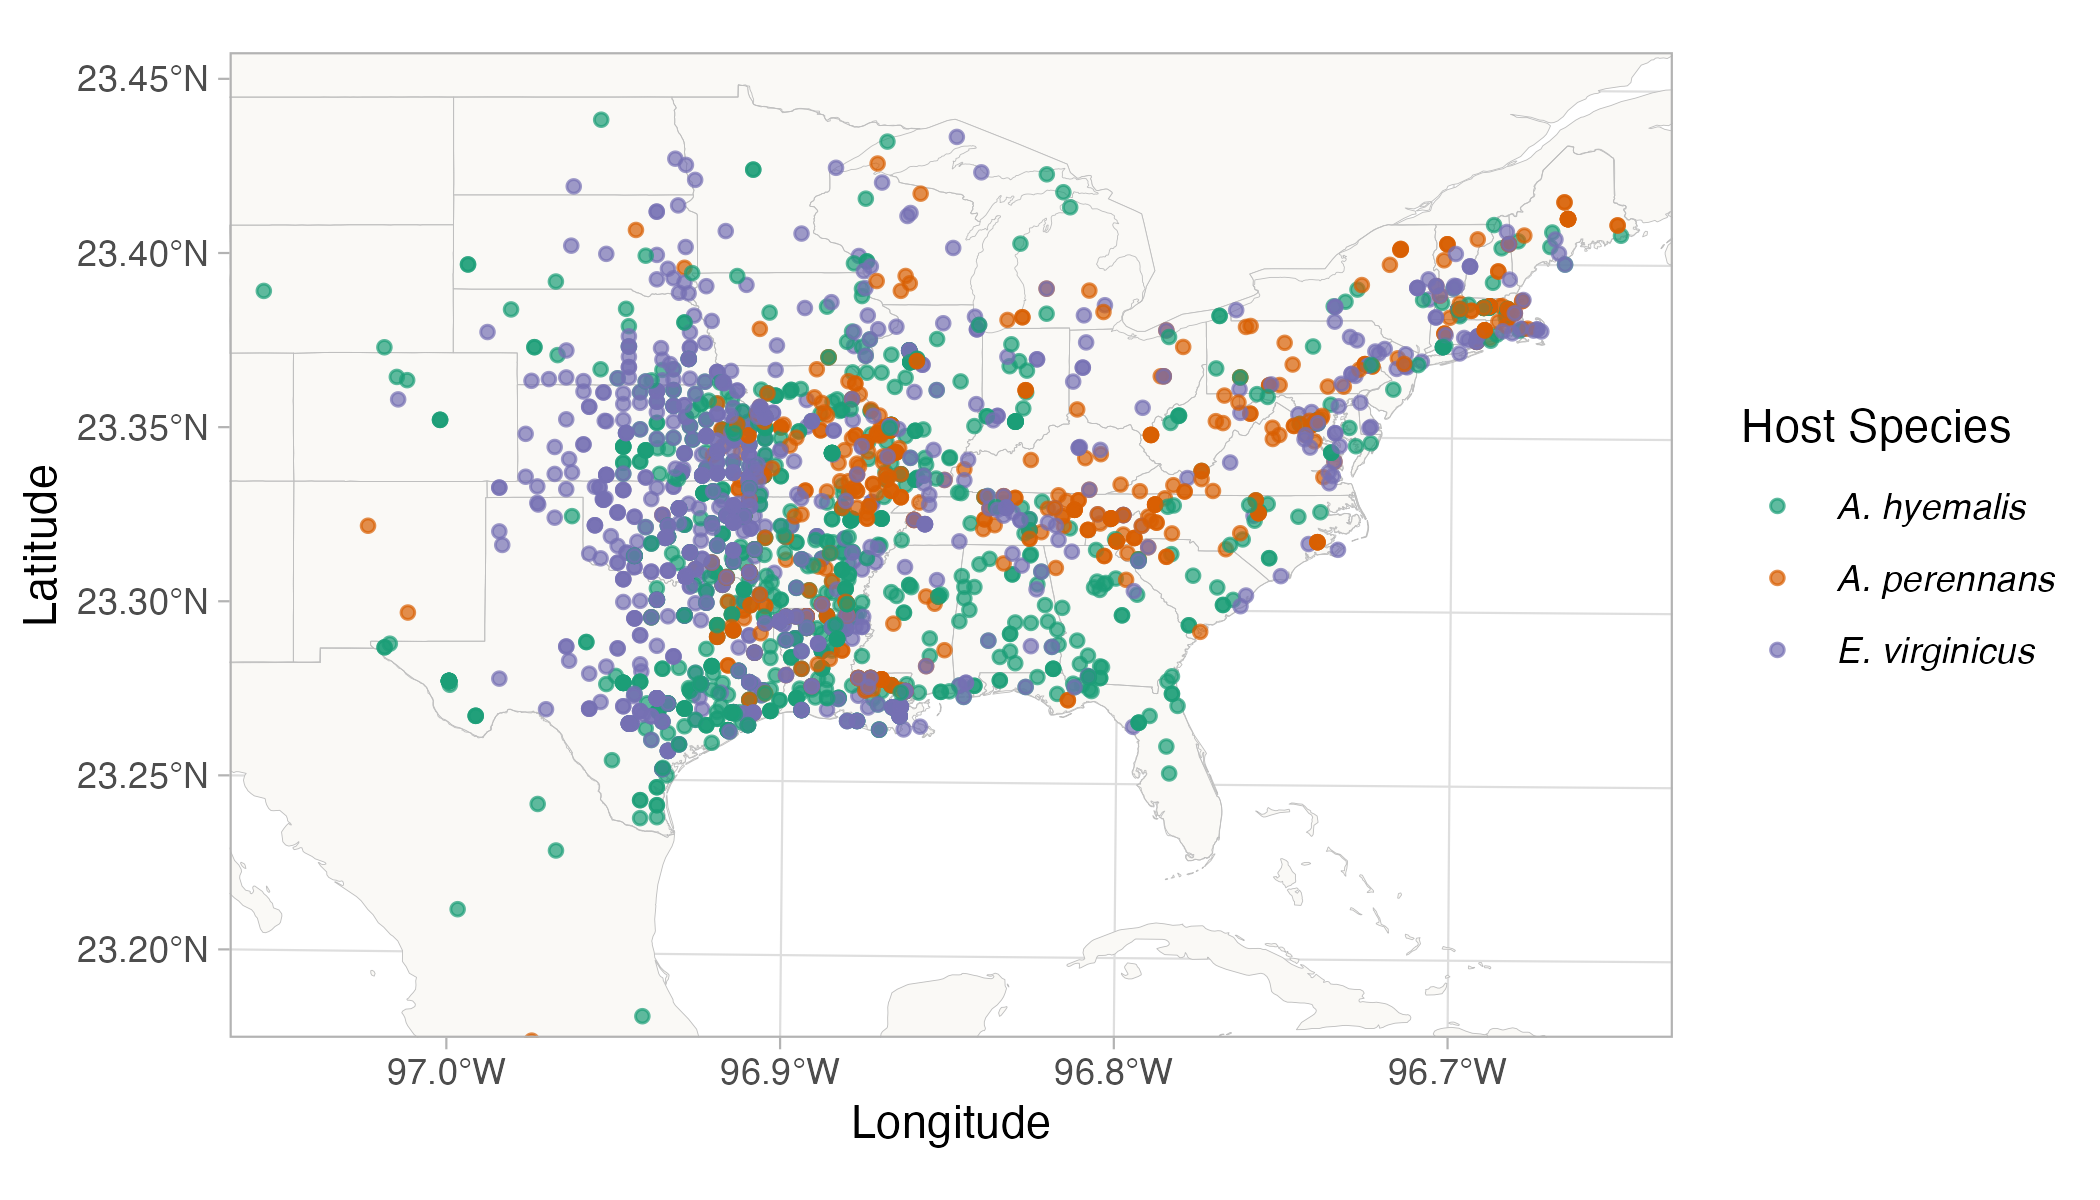
\includegraphics[width = \linewidth]{../Plots/collections_map.png}
	\caption{\textbf{Collection locations of herbarium specimens of three grass host species across eastern North America that were sampled for \emph{Epichloë} endophyte presence or absence}.}
	\label{fig:map}
\end{figure}


\subsection*{Modeling spatial and temporal changes in endophyte prevalence}
We assessed spatial and temporal changes in endophyte prevalence across each host distribution, quantifying the ``global'' temporal trends, aggregating across space, and then examining spatial heterogeneity in the direction and magnitude of endophyte change (hotspots and coldspots) across the spatial extent of each host's distribution.
To appropriately account for the spatial non-independence of geo-referenced \josh{occurrences}{spelling?}, we used an approximate Bayesian method, Integrated Nested Laplace Approximation (INLA), to construct spatio-temporal models of endophyte prevalence.
INLA provides a computationally efficient method of ascertaining parameter posterior distributions for certain models that can be formulated as latent Gaussian Models \cite{rue2009approximate}.
Many common statistical models, including structured and unstructured mixed-effects models, can be represented as latent Gaussian Models.
We incorporated spatial heterogeneity into this analysis using spatially-structured intercept and slope parameters implemented as stochastic partial differential equation (SPDE) approximations of a continuous spatial Gaussian process. 
This SPDE approach is a flexible method of smoothing across space while explicitly accounting for spatial dependence between data-points \citep{lindgren2011explicit,bakka2018spatial}.
Fitting models with structured spatial effects is possible with MCMC sampling but can require long computation times, making INLA an effective alternative, which has been used to model spatial patterns in flowering phenology \cite{willems2022forest}, the abundance of bird species \cite{meehan2019spatial} and butterflies \cite{crossley2022opposing}, the distribution of temperate trees \cite{engel2022spatial} as well as the population dynamics of endangered amphibians \cite{knapp2016large} and other ecological processes \cite{beguin2012hierarchical}.

We estimated global and spatially-varying trends in endophyte prevalence using a joint-likelihood model. 
For each host species $h$, endophyte presence/absence of the $i^{th}$ specimen ($P_{[h]i}$) was modeled as a Bernoulli response variable with expected probability of endophyte occurrence $\hat{P}_{[h]i}$.
We modeled $\hat{P}_{[h]i}$ as a linear function of intercept $ \mathrm{A}_{[h]i}$ and slope $\mathrm{T}_{[h]}$ defining the global trend in endophyte prevalence specific to each host species as well as with spatially-varying intercepts $\alpha_{[h_{1}]l[i]}$ and slopes $\tau_{[h_{1}]l[i]}$ associated with location ($l[i]$, a unique latitude-longitude combination).
The joint-model structure allowed us to share variance terms across focal species to account for dependence associated with the collection of specimens and identification of endophytes. 
Shared variance terms included the spatially-dependent random effect $\delta_{l[i]}$, intended to account for residual spatial variation, and $\chi_{c[i]}$ and $\omega_{s[i]}$ i.i.d.-random effects indexed for each collector identity ($c[i]$), and scorer identity ($s[i]$) of the $i^{th}$ specimen.
\begin{subequations}
	\label{eq:trends}
	\begin{align}
		logit(\hat{P}_{[h_{1}]i}) =  \mathrm{A}_{[h_{1}]i} + \mathrm{T}_{[h_{1}]}*year_i  + \alpha_{[h_{1}]l[i]} + \tau_{[h_{1}]l[i]}*year_i  + \delta_{l[i]}+ \chi_{c[i]} + \omega_{s[i]} \\
		logit(\hat{P}_{[h_{2}]i}) = \mathrm{A}_{[h_{2}]i} + \mathrm{T}_{[h_{2}]}*year_i  + \alpha_{[h_{2}]l[i]} + \tau_{[h_{2}]l[i]}*year_i  + \delta_{l[i]}+ \chi_{c[i]} + \omega_{s[i]} \\
		logit(\hat{P}_{[h_{3}]i}) = \mathrm{A}_{[h_{2}]i} + \mathrm{T}_{[h_{2}]}*year_i  + \alpha_{[h_{2}]l[i]} + \tau_{[h_{3}]l[i]}*year_i  + \delta_{l[i]}+ \chi_{c[i]} + \omega_{s[i]}
	\end{align}
\end{subequations}


Previous work suggests that behavior of historical botanists and uneven sampling may introduce biases into ecological inferences made from historic collections \cite{kozlov2020biases}. 
Prolific collectors who contribute thousands of specimens may be more or less likely to collect certain species, or specimens with certain traits \cite{daru2018widespread}. 
Similarly, the process of scoring seeds for hyphae involved several student researchers who, even with standardized training, may vary in their likelihood of positively identifying \emph{Epichloë} hyphae. 
By including a random effect for collectors and for scorers, we attempted to account for variance across individual researchers that may bias our predictions of changes in endophyte prevalence.


We performed model fitting using the inlabru R package \citep{}\jacob{} {add citation}.
Global intercept and slope parameters $\mathrm{A}$, and $\mathrm{T}$, were given vague priors.
Scorer and collector random effects, $\chi$ and $\omega$, were given penalized complexity priors, with distributions approximating a Normal distribution with standard deviation of 5. 
Each spatially-structured parameter depended on a covariance matrix according to the proximity of each collection location \citep{lindgren2011explicit,bakka2018spatial}. 
The covariance matrix was approximated using a Mat\'{e}rn covariance function, with each data point assigned a location according to the nodes of a mesh of non-overlapping triangles encompassing the study area (Fig. \ref{fig:meshplot}).
Priors, termed ''range" and "variance", define the distance of spatial decay described by the Mat\'{e}rn covariance function.
Priors for results presented in the main text reflect a range of \josh{XX}{} kilometers. 
We found that model results were sensitive to this choice, and so tested a range of priors (from XX kilometers to XX kilometers) and meshes (Supplemental Material), finding that model results were qualitatively similar, i.e. the same direction of effects across space, but that the magnitude and uncertainty varied. 
%In all cases, posterior modes were \tom{stable}{Assessed how?} and equal to zero, indicating successful numeric convergence.


\subsection*{Validating model performance with in-sample and out-of-sample tests}
We evaluated the predictive ability of the model using both in-sample training data from the herbarium surveys, and with out-of-sample test data from contemporary endophyte surveys, \tom{an important but rarely used strategy in ecological studies \cite{tredennick2021practical}.}{This is the type of thing to emphasize in the intro? Are there any other collections-based papers that have done anything like this?? None to my knowledge.} \josh{}{Add Benjamin lee paper, maybe? it's not just herbaria, but kind of related}
We used data from contemporary surveys of endophyte prevalence  in \emph{A. hyemalis} and \emph{E. virginicus} in Texas and the southern US. 
Surveys of \emph{E. virginicus} were conducted in 2013 as described in \citet{sneck2017variation}, and \tom{surveys of \emph{A. hyemalis} took place between 2015 and 2020}{We have added more recent AGHY survey data. I am not sure if you have access to this but you should definitely use it. Karl or I can point you to the right file.}.
Population surveys of \emph{A. hyemalis} were initially designed to cover longitudinal variation in endophyte prevalence towards its range edge, while surveys of \emph{E. virginicus} were designed to cover latitudinal variation along its range edge. 
In total, we visited 43 populations of \emph{A. hyemalis} and 20 populations of \emph{E. virginicus} across the south-central US, with emphasis on Texas and neighboring states (Fig \ref{fig:contempsurveysmap}).
During surveys, we collected seeds from up to 30 individuals per location  (average number of plants sampled: $22.9$).
We quantified the endophyte status of each individual with staining microscopy as described for the herbarium surveys (with 5-10 seeds scored per individual), and calculated the prevalence of endophytes within the population (proportion of symbiotic plants divided by the number of sampled plants).
For each population, we compared the observed fraction of endophyte-symbiotic hosts to the predicted probability of endophyte occurrence $\hat{P}$ derived from the model based on location and year. 
The contemporary survey period (2013-2020) is at the most recent edge of the time period encompassed by the historical observations used for model fitting.
We compared the model's prediction for these locations to the observed population prevalence.

\subsection*{Assessing the role of climate drivers}
We assessed how the magnitude of climate change may have driven changes in endophyte prevalence by assessing correlations between changes in climate and changes in endophyte prevalence predicted from our spatial model at evenly spaced pixels across the study area.
We first downloaded monthly temperature and precipitation rasters from the PRISM climate group \citep{daly2013prism} covering the time period between 1895 and 2020 using the 'prism' R package \citep{Rprism2015}. 
Prism provides reconstructions of historic climate variables across the United States by spatially-interpolating weather station data \citep{diLuzio2008constructing}. 
We calculated 30-year climate normals for seasonal mean temperature and cumulative precipitation for the recent (1990 to 2020) and historic (1895 to 1925) periods.
We used three four-month seasons within the year (Spring: January, February, March, April; Summer: May; June, July, August; Autumn: September, October, November, December). 
This division of seasons allowed us to quantify differences in climate associated with the two ``cool'' seasons, when we expected our focal species to be most biologically active (\emph{A. hyemalis} flowering phenology: spring; \emph{E. virginicus}: spring and summer; \emph{A. perennans}: autumn). 
In addition to mean climate conditions, environmental variability itself can influence population dynamics \cite{tuljapurkar_population_1982} and changes in variability are a key prediction of climate change models \cite{stocker2013technical, ipcc_2021}.
Therefore, we calculated the standard deviation for each annual and seasonal climate driver across each 30-year period.
We then took the difference between recent and historic periods for the mean and standard deviation for each climate driver (Figs. \ref{fig:AGHY_climate_covariates}-\ref{fig:ELVI_climate_covariates}).
%Because initial analyses indicated a high degree of collinearity between seasonal and annual changes in temperature, we used annual temperature only, along with annual and seasonal precipitation, in the subsequent analysis.
All together, we assessed twelve potential climate drivers: the mean and standardization of spring, summer, and autumn temperature, as well as the mean and standard deviation of spring, summer, and autumn cumulative precipitation, cumulative precipitation, and cumulative precipitation.

To evaluate whether areas that have experienced the greatest changes in endophyte prevalence (hotspots of endophyte change) are associated with high degrees of change in climate (hotspots of climate change), \tom{we modeled spatially varying slopes of endophyte change through time ($\tau_{[h]l}$ as a linear function of environmental covariates, with a Gaussian error distribution. }{I think we need to account for uncertainty in the slopes. They are outputs of a (quasi) Bayesian model so we should be able to propagate all the uncertainty in the posterior distribution.}
Data from each host species was analyzed separately. 
Fitting regressions to many pixels across the study region risks artificially inflating confidence in our results due to large sample sizes, and \tom{so we performed this analysis using only a random subsample of 250 pixels across the study region, which provided results qualitatively similar to analysis of the full set of pixels}{100 seems like a low number to me. What if we did this for all of the herbarium collection locations?}\josh{.}{I upped the number of points. I don't think conceptually we need to only do collection locations, but I can work on that as an alternative.}


\tom{}{I cut the notation for the Gaussian model for now because it is a pretty simple model and the notation may be overkill, plus because I changed your tau's to beta's there were betas on both sides of the tilde, which was confusing/annoying. Happy have the notation back if you prefer it. I am also a little confused because the appendix has spearman correlations but there are no methods here for where those come from.}


\subsection*{Modeling distributions of host species}
We modeled the distribution of each host species to generate maps on which we predicted the dynamics of \emph{Epichloë} symbionts.
We followed the ODMAP (overview, data, model, assessment, prediction) protocol \citep{crossley2022opposing}. 
 A full description of the ODMAP can be found in the  (Supplementary Method \ref{sec:sdm }). 
 Here we presented the workflow of the species distribution model. 
 We used presence-only observations of the host species from Global Biodiversity Information Facility (GBIF) between 1990 to 2020.
To reduce the potential influence of sampling bias and spatial autocorrelation, we thinned the occurrences to the spatial scale of our selected climatic predictors. 
We selected climate variables that aligned with our analysis of climatic influences on trends in endophyte prevalence described above.
These climatic variables are: the mean and standard deviation of spring, summer, and autumn temperature, as well as the mean and standard deviation of spring, summer, and autumn cumulative precipitation, cumulative precipitation, and cumulative precipitation.
%We calculated the mean and standard deviation of seasonal temperature and precipitation across 1990 to 2020. 
Among this suite of variables, we chose to include mean summer temperature, standard deviation of spring temperature, standard deviation of summer temperature,  standard deviation of spring  precipitation, standard deviation of summer  precipitation, which were uncorrelated (Variance Inflation Factor $>$ 0.7) and allowed us to predict the occurrence probability of each host species in space and time.
We fit maximum entropy (MaxEnt) models using the maxent function in the package dismo \citep{hijmans2017package}. 
%\josh{MaxEnt is preferred because it has been shown to generate response curves with less unpredictable behavior when applied to new climates \citep{hijmans2006ability}.}{possibly could remove this sentence?}
We generated 10,000 pseudo-absences as background points, and split the occurrence data into 75\% for model training and 25\% for model testing.
The performance of models was evaluated with AUC  \citep{jimenez2012insights}. 
We found AUC = 0.862, AUC = 0.838, AUC = 0.821 respectively  for \emph{Agrostis hyemalis}, \emph{Agrostis perennans}, and \emph{Elymus virginicus}. 

To convert the continuous predicted probabilities into binary presence - absence maps, we used the  training sensitivity (true positive rate) and specificity threshold (true negative rate) \citep{liu2005selecting}. 
These binary maps serve as boundaries in presented maps of change in endophyte prevalence, and outline the set of pixels used in our analysis of climate correlates with trends in endophyte prevalence.

		
\section*{Results}
\subsection*{How has endophyte prevalence changed over time?}
We found that endophyte prevalence increased within the examined specimens over the last two centuries for all three host species (Fig. \ref{fig:temporal}). 
On average, modeling indicated that endophytes of \emph{A. perennans} and \emph{E. virginicus} increased from $\sim 40$ \% to  $70$\% prevalence across the study region, and that of \emph{A. hyemalis} increased from $\sim 25$\% to over $50$\% prevalence.
Our model indicates a high certainty that overall temporal trends are positive across species (99\% probability of a positive overall year slope in \emph{A. hyemalis}, 92\% probability of a positive overall year slope in \emph{A. perennans}, and 91\% probability of a positive overall year slope in \emph{E. virginicus}) (Fig. \ref{fig:temporal_posterior})

\begin{figure}[H]
	\centering
	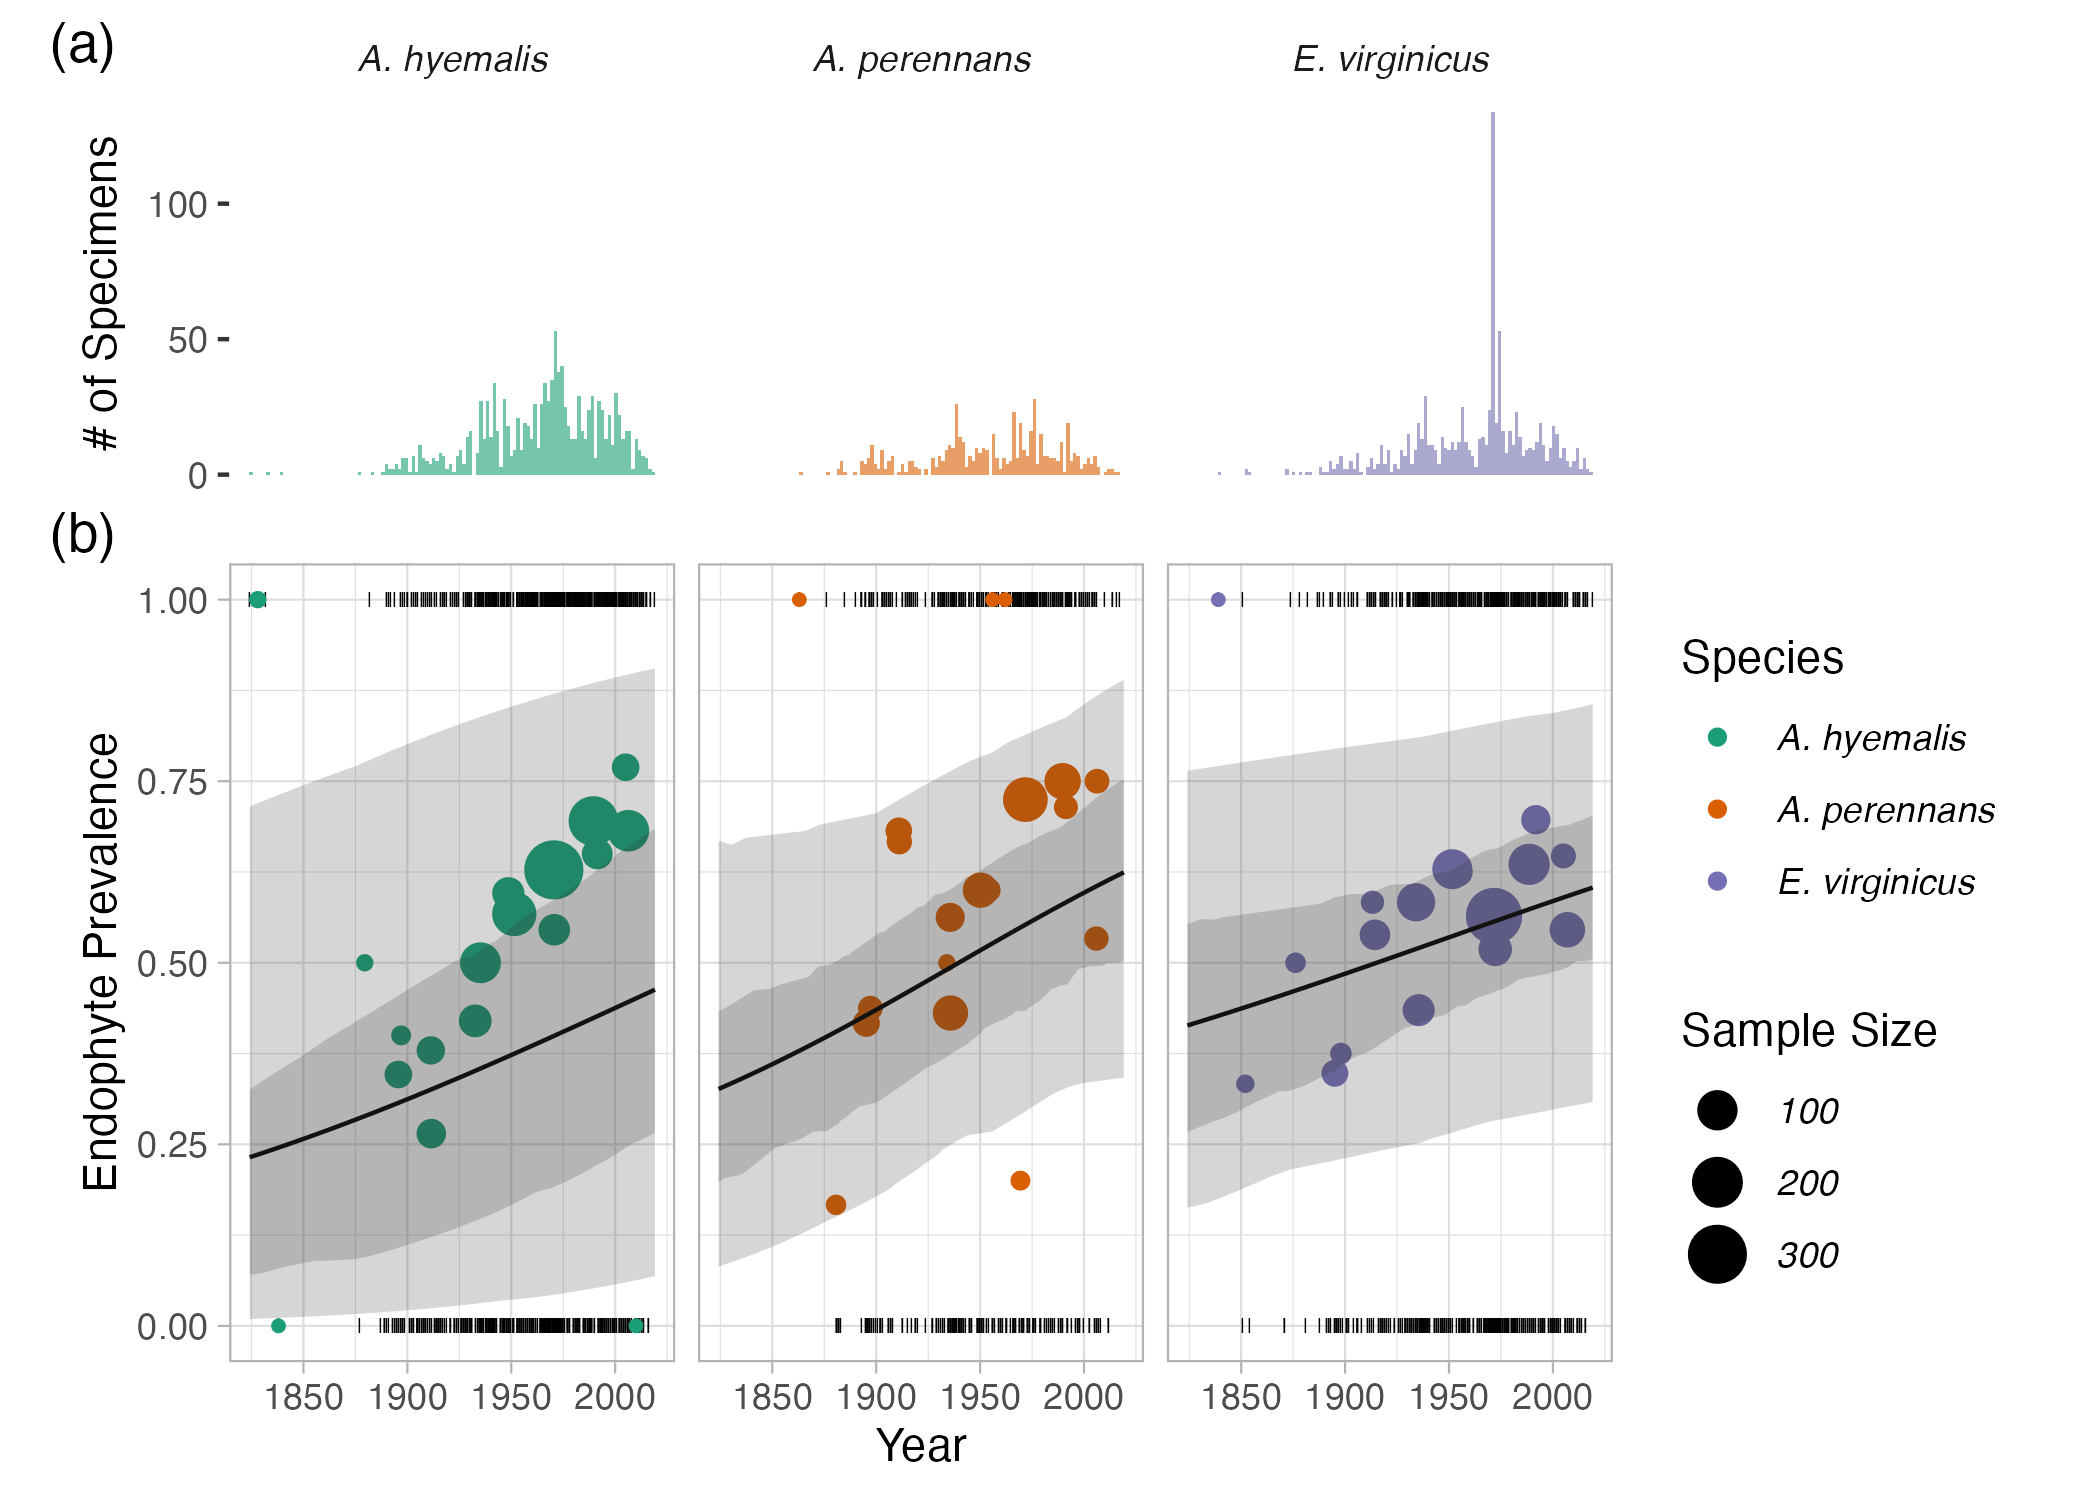
\includegraphics[width = \linewidth]{../Plots/year_plot.png}
	\caption[Temporal trends in endophyte prevalence.]{Temporal trends in endophyte prevalence. (A) Histograms show the frequency of scored specimens through time for each host species. (B) Lines show predicted mean endophyte prevalence over the study period along with the 50\%  and 95\% CI bands incorporating uncertainty associated with collector and scorer random effects. Colored points are binned means of the observed endophyte presence/absence data (black dashes). Colors represent each host species and point size represents the number of specimens.}
	\label{fig:temporal}
\end{figure}




\subsection*{How spatially variable are temporal trends in endophyte prevalence?}
Our model revealed hotspots of change in endophyte prevalence. 
While there was an overall increase in endophyte prevalence, these changes varied across the host species' ranges (Fig. \ref{fig:svc_time_map}).
In some regions, posterior estimates of spatially varying temporal trends, $\tau$, indicate that \emph{A. hyemalis} and \emph{A. perennans} experienced increases in percent prevalence by as much as $2$\% per year over the study period, while  \emph{E. virginicus} experienced increases up to around $1$\% per year. 
Compared to \emph{E. virginicus}, which had a weaker overall increase in endophytes and less spatial variability, maps of both \emph{Agrostis} species show areas of strong increase and areas of declining prevalence.
Notably, endophytes increased towards the western range edge of \emph{A. hyemalis} (Fig. \ref{fig:svc_time_map}A) and across the northeastern US for \emph{A. perennans} (Fig. \ref{fig:svc_time_map}B). 
Posterior estimates of uncertainty in spatially varying slopes indicate that these hotspots of change may have experienced increases of up to $5$\% per year while declines in prevalence may be as great as $4$\% per year for \emph{A. hyemalis} and \emph{A. perennans}.
For \emph{E. virginicus}, uncertainty ranges between $3.5$\% increases and $2.5$\% decreases (Fig. \ref{fig:svc_time_map_CI}).

\begin{figure}[H]
	\centering
	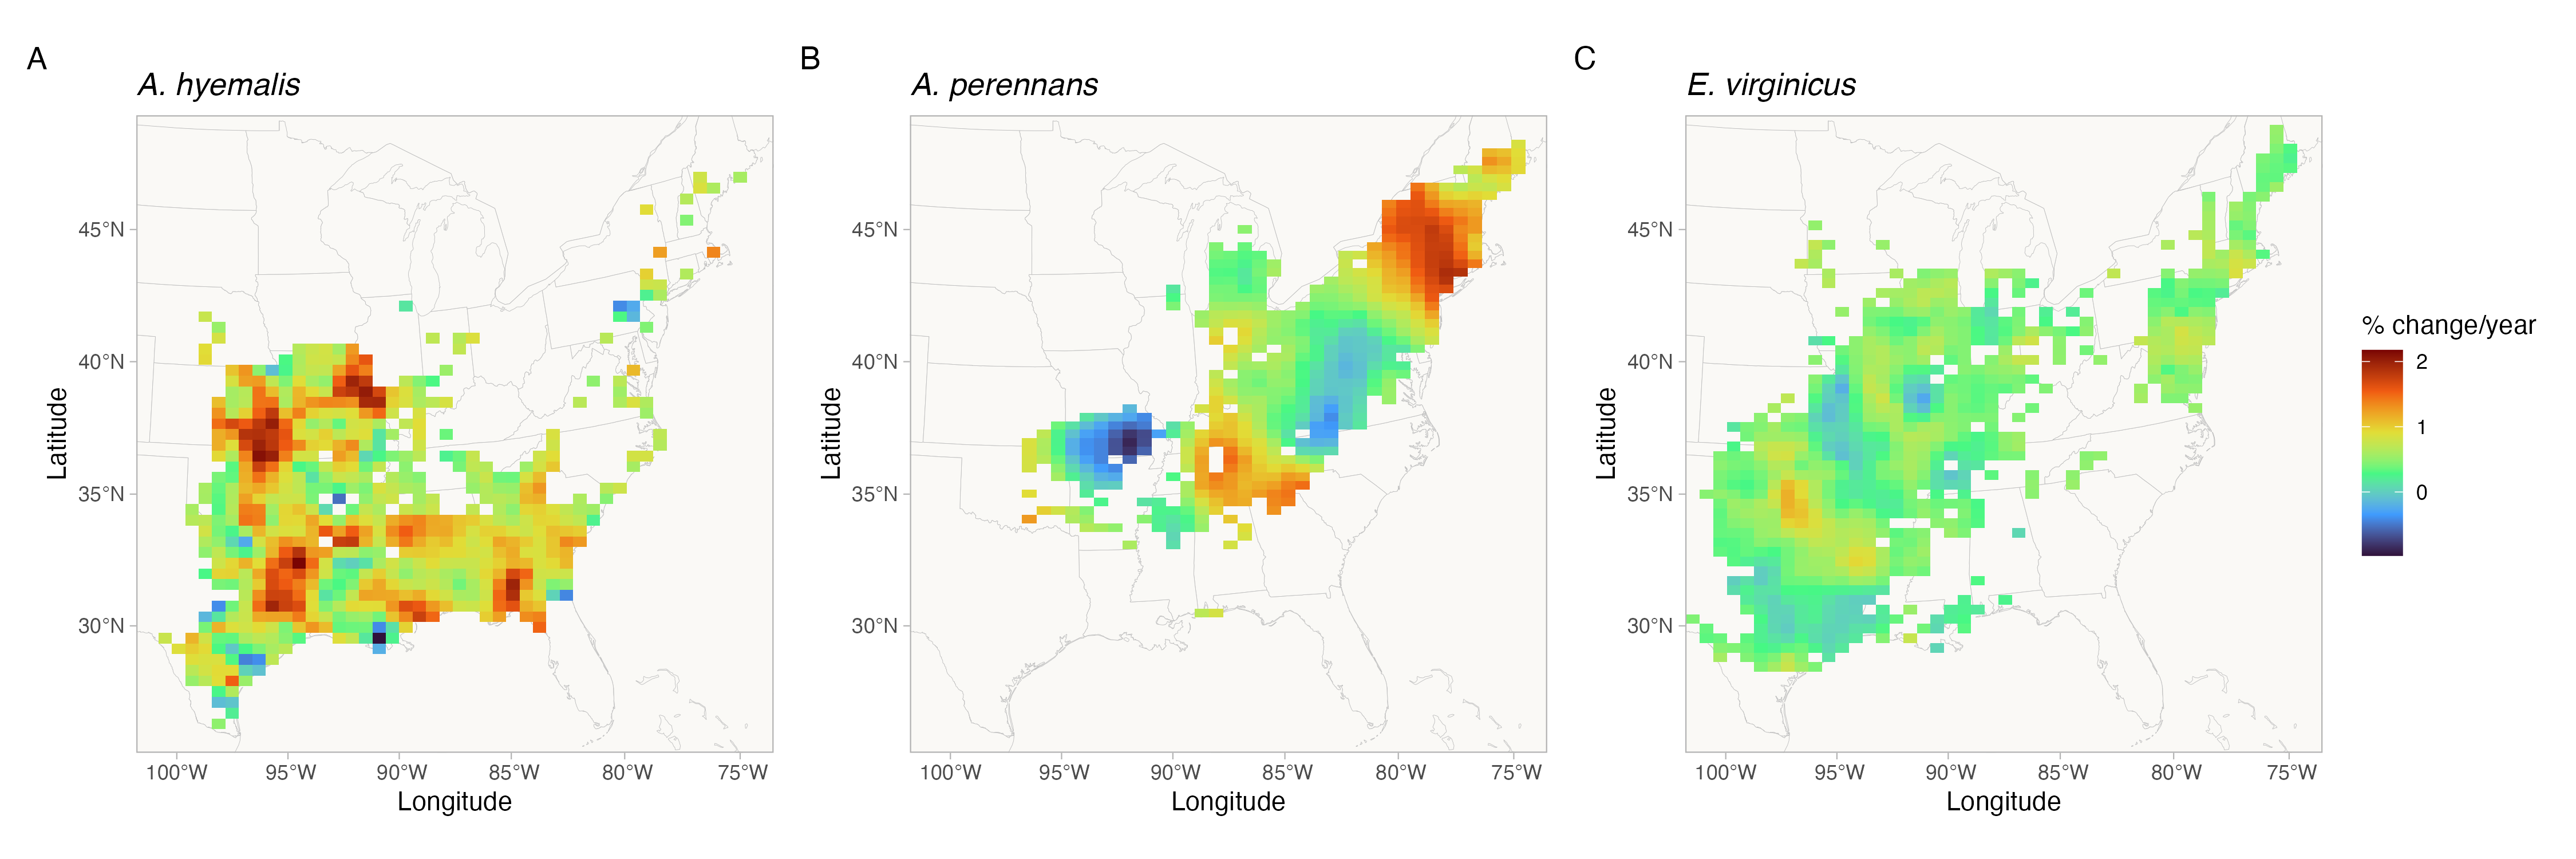
\includegraphics[width = \linewidth]{../Plots/svc_time_map.png}
	\caption[Predicted posterior mean of spatially-varying slopes representing change in endophyte prevalence for each host species.]{Predicted posterior mean of spatially-varying slopes representing change in endophyte prevalence for each host species. Color indicates the relative change in predicted endophyte prevalence.}
	\label{fig:svc_time_map}
\end{figure}



%\subsubsection*{How does endophyte prevalence vary across space?}
%Across space, there were clear trends in endophyte prevalence which varied between species (Fig. 5).
%We mapped predictions of endophyte prevalence across the area encompassing the sampled herbarium specimens for each species, and area smaller than the full geographic distribution of each species in nature.
%\emph{Elymus virginicus} had higher prevalence towards the northern portions of the collection range. 
%In contrast, \emph{Agrostis hyemalis} had highest prevalence towards the center of its collection range with regions of low prevalence towards the northeast and towards its western range edge.
%\emph{Agrostis perennans} had  highest prevalence towards the westernmost portion of its collection range.
%There is considerable uncertainty in the spatial pattern of endophyte prevalence (See Fig. A10 for projections of the 95\% credible interval), however these broad spatial patterns are consistent across the low and high end of model predictions. 

%\begin{figure}[H]
%	\label{fig:svc_space_map}
%	\centering
%	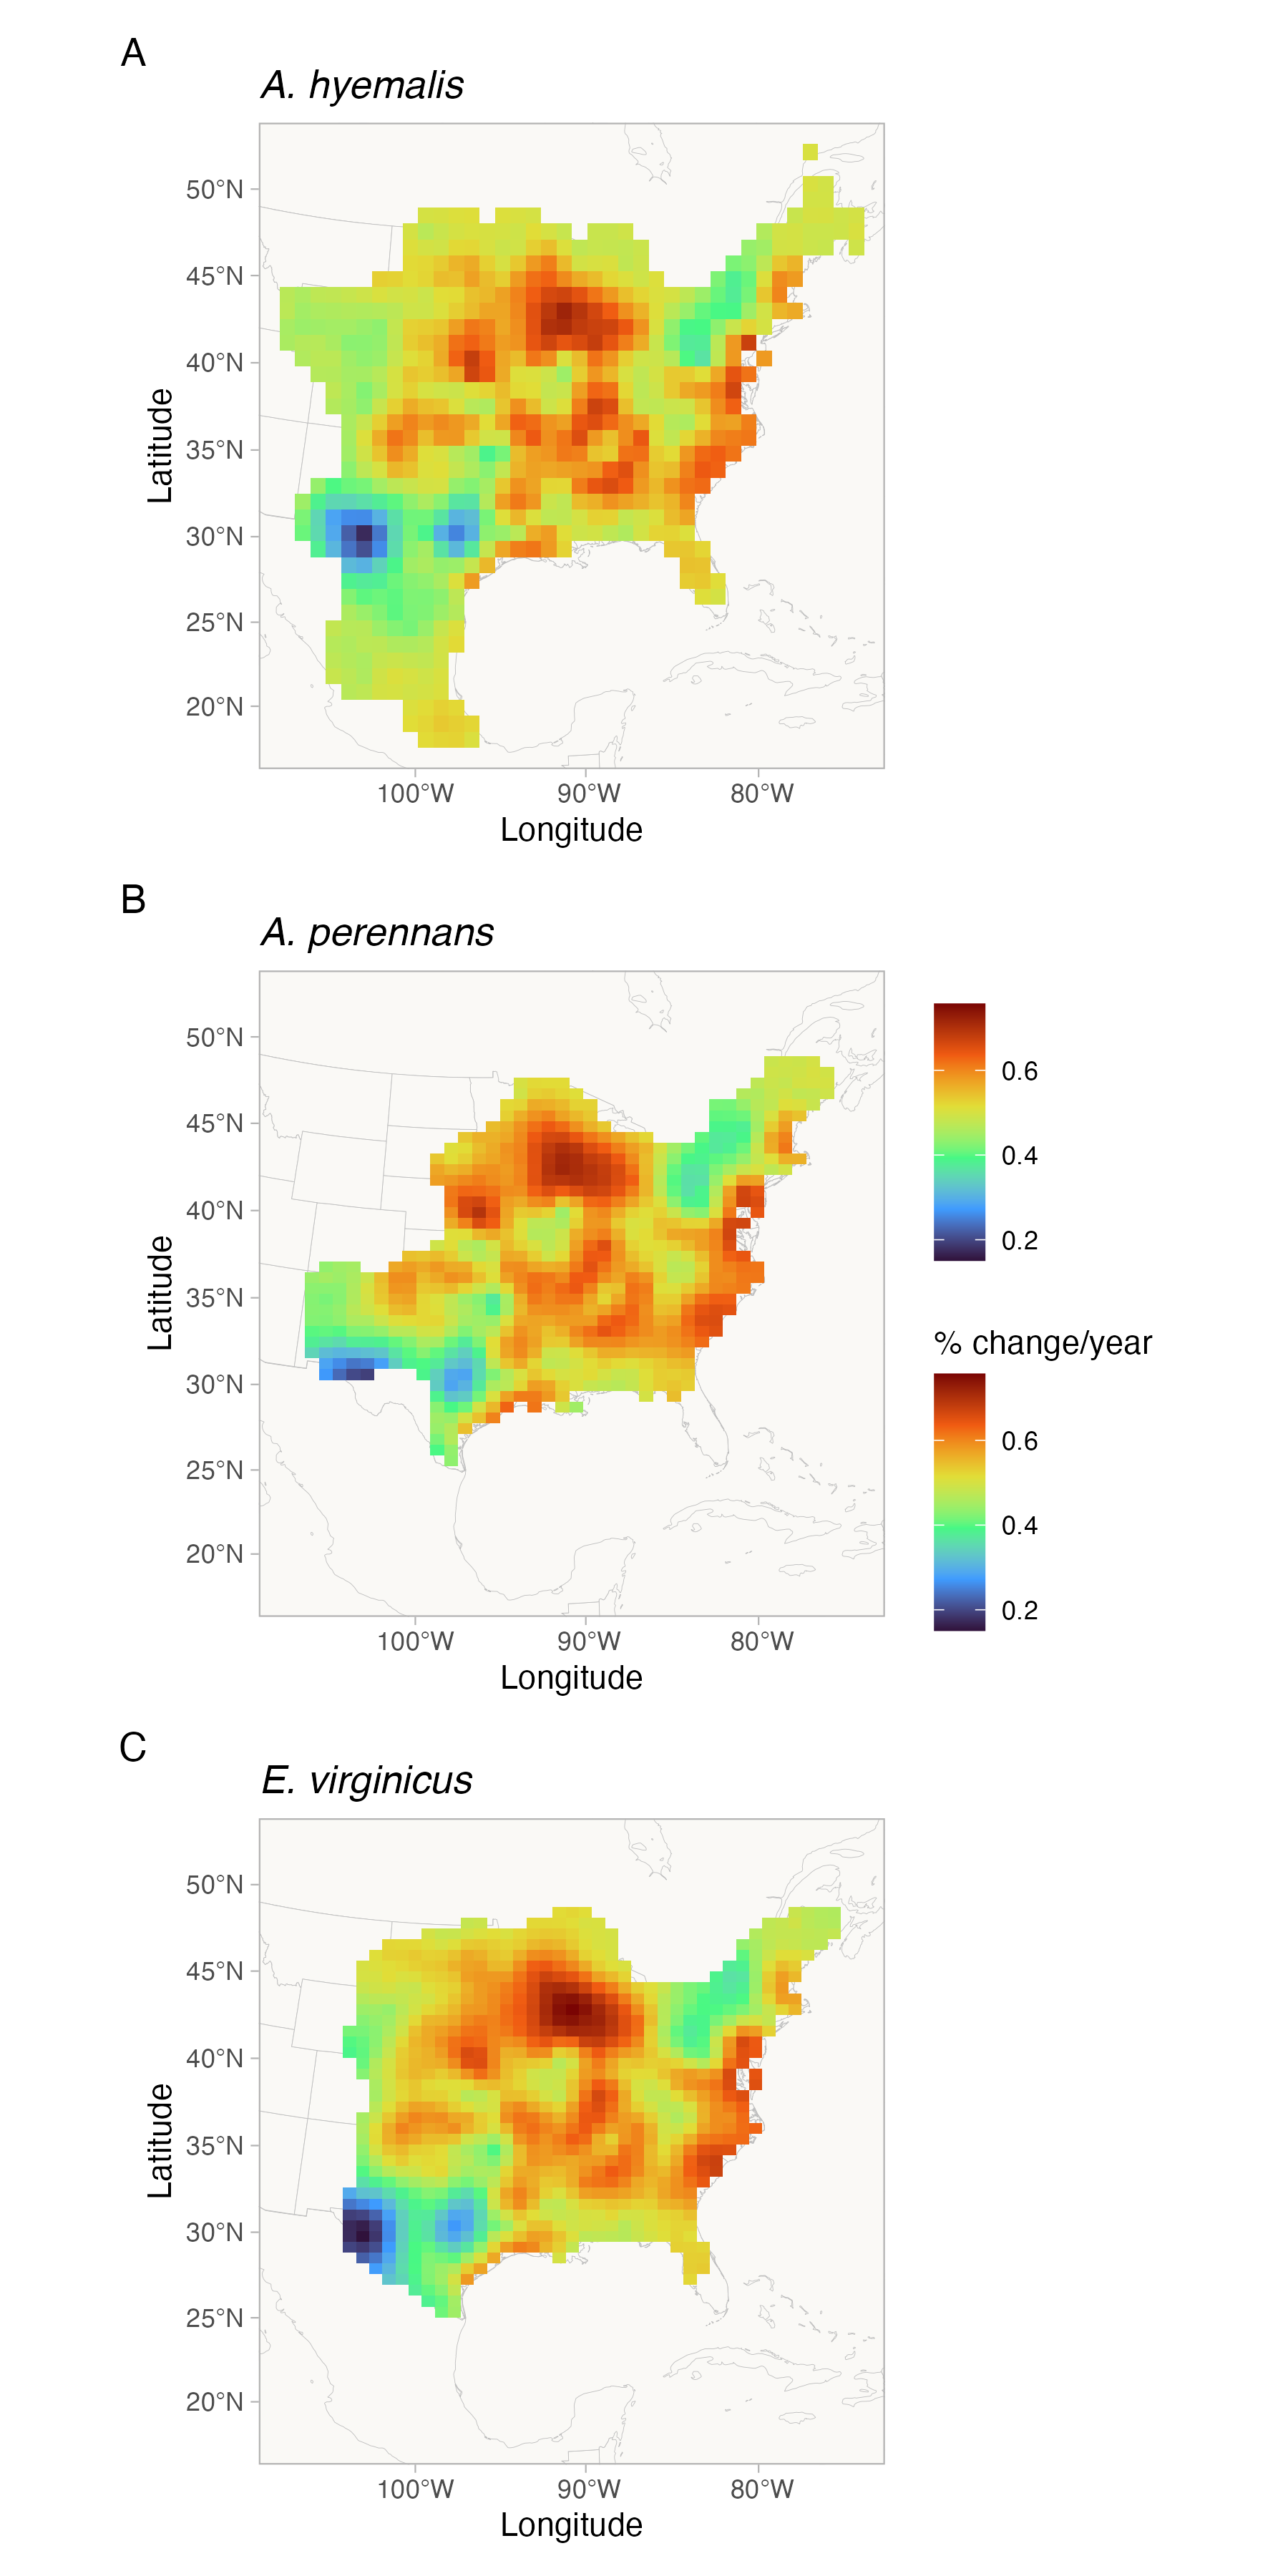
\includegraphics[width = .6\linewidth]{svc_space_map.png}
%	\caption{\textbf{Mean predicted endophyte prevalence for each host species (columns) in 1925 (top row) and 2020 (bottom row)}. Color indicates mean predicted rate of endophyte prevalence across the predicted distribution of each species.}
%\end{figure}





\subsection*{What is the relationship between variation in temporal trends in endophyte prevalence and changes in climate drivers?}

We found that trends in endophyte prevalence were strongly associated with seasonal climate change drivers (Fig. \ref{fig:climate_correlation_plot}).
For the majority of the study region, the climate has become wetter and cooler over the last century (Fig. \ref{fig:AGHY_climate_covariates}-\ref{fig:ELVI_climate_covariates}), a consequence of regional variation in global climate change \cite{ipcc_2021}. 
Within the study region, spatial variation in climate trends were predictive of trends in endophyte prevalence.
For example, strong increases in prevalence within \emph{A. perennans} were most associated with autumn climate drivers that coincide with its Aug-Sep active growing season. 
For this species, warmer and wetter autumn climates showed particularly strong relationships, however other seasonal drivers may also contribute to increasing endophyte prevalence (drier springs and cooler summers).
Trends in endophyte prevalence for \emph{A. hyemalis} were most strongly associated with changes in precipitation variability were the strongest predictors.
Endophyte prevalence increased the most in regions that experienced greater spring precipitation along with increasing variability in summer and autumn precipitation. 
While this species actively grows and reproduces in the late spring and early summer, climate effects outside of the growing season may indicate that endophytes play a role in persistence during dormant periods through summer droughts or contribute to the ability to successfully germinate.
Prevalence of endophytes of \emph{E. virginicus} were least influenced by climate, but decreasing autumn temperature variability and less precipitation in autumn were the strongest predictors.


Correlations assessed using all pixels across each species distribution were qualitatively similar to these results (Fig. A11).
%These associations are in line with expectations that endophyte symbiosis provides drought tolerance to their hosts, particularly during \emph{E. virginicus}'s \tom{summer growing season}{It is a stretch to say that this species has a summer growing season.}. 
%For \emph{A. perennans}, which flowers in the late Summer and Autumn, increases in autumn precipitation along with increases in variability in annual precipitation, were strongly assocated with increasing endophyte prevalence.  
%While this result is contrary to the expectation that endophyte provide drought tolerance, this species typically is associated with wetter microhabitats, and it also \tom{suggests a role for endophytes to play in buffering the negative consequences of demographic variability \citep{lewontin_population_1969}}{I would save for discussion}.  
%For \emph{A. hyemalis}, which flowers in the Spring, changes in endophyte prevalence were more weakly associated with seasonal changes in climate drivers than for the other two species.
%It was, however, the only species' for which greater increases in endophyte prevalence were associated with regions that experienced increases in average annual temperatures.\tom{}{Is this a significant association, however you want to define that? Or could this result have occurred by chance?}

\begin{figure}[H]
	\centering
	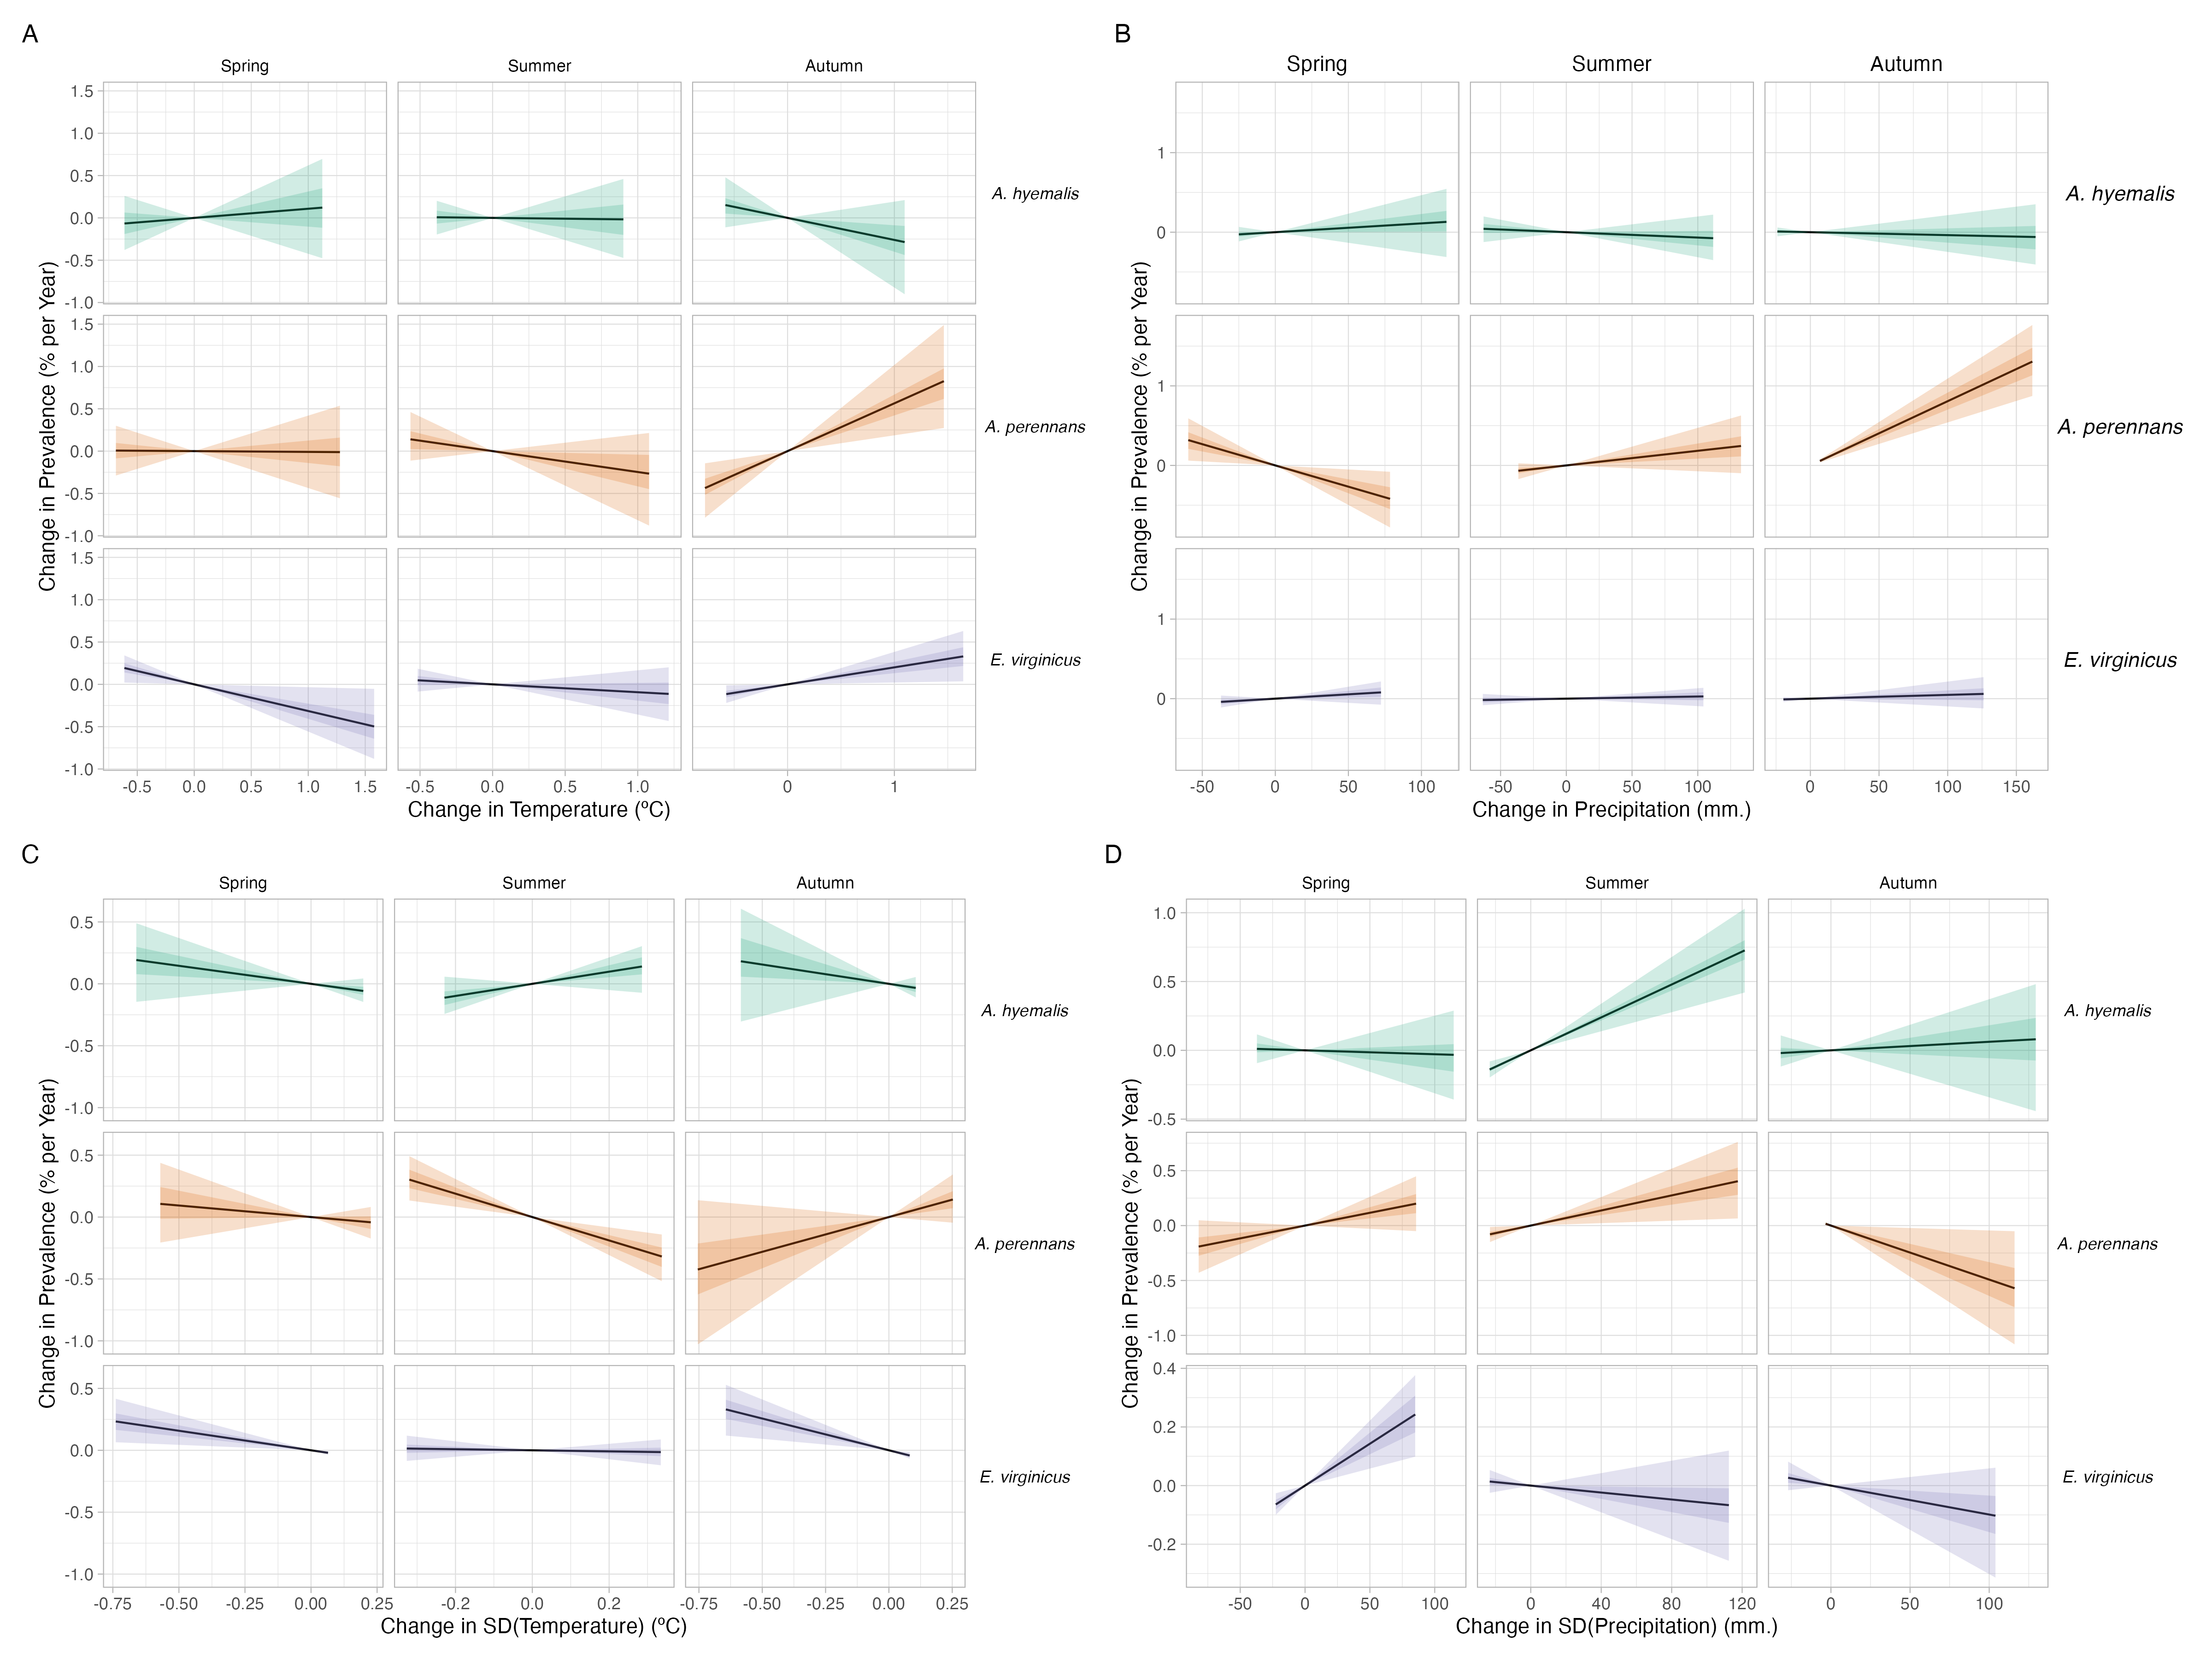
\includegraphics[width = \linewidth]{../Plots/climate_trends_plot.png}
	\caption{\textbf{Relationships between changes in seasonal climate drivers and predicted marginal trends in endophyte prevalence.} Lines show relationships between seasonal climate (A: mean temperature, B: cumulative precipitation, C: standard deviation in temperature, D: standard deviation in precipitation) and spatially-varying trends in endophyte prevalence for each host species, along with 50 and 95\% CI.}
	\label{fig:climate_correlation_plot}
\end{figure}




\subsubsection*{Performance on test data}
We found that model performance, as judged by AUC, was similar between historic herbarium specimens used as training data and the out-of-sample test data from contemporary surveys (0.79 and 0.77 respectively; Fig. \ref{fig:ROCtest}-\ref{fig:ROCtraining}).  
The model successfully captured broader regional trends in endophyte prevalence present in the contemporary survey data, such as decline endophyte prevalence towrads western longitudes in \emph{A. hyemalis}  (Fig. \ref{fig:contemptestplot}A). 
However, the contemporary data contains additional variability at smaller scales not captured by our sampling of herbarium specimens. 
We interpreted this to mean that the model captured regional spatial dynamics, but underpredicts local scale dynamics.
We discuss potential model improvements in the Discussion.

\begin{figure}[H]
	\centering
	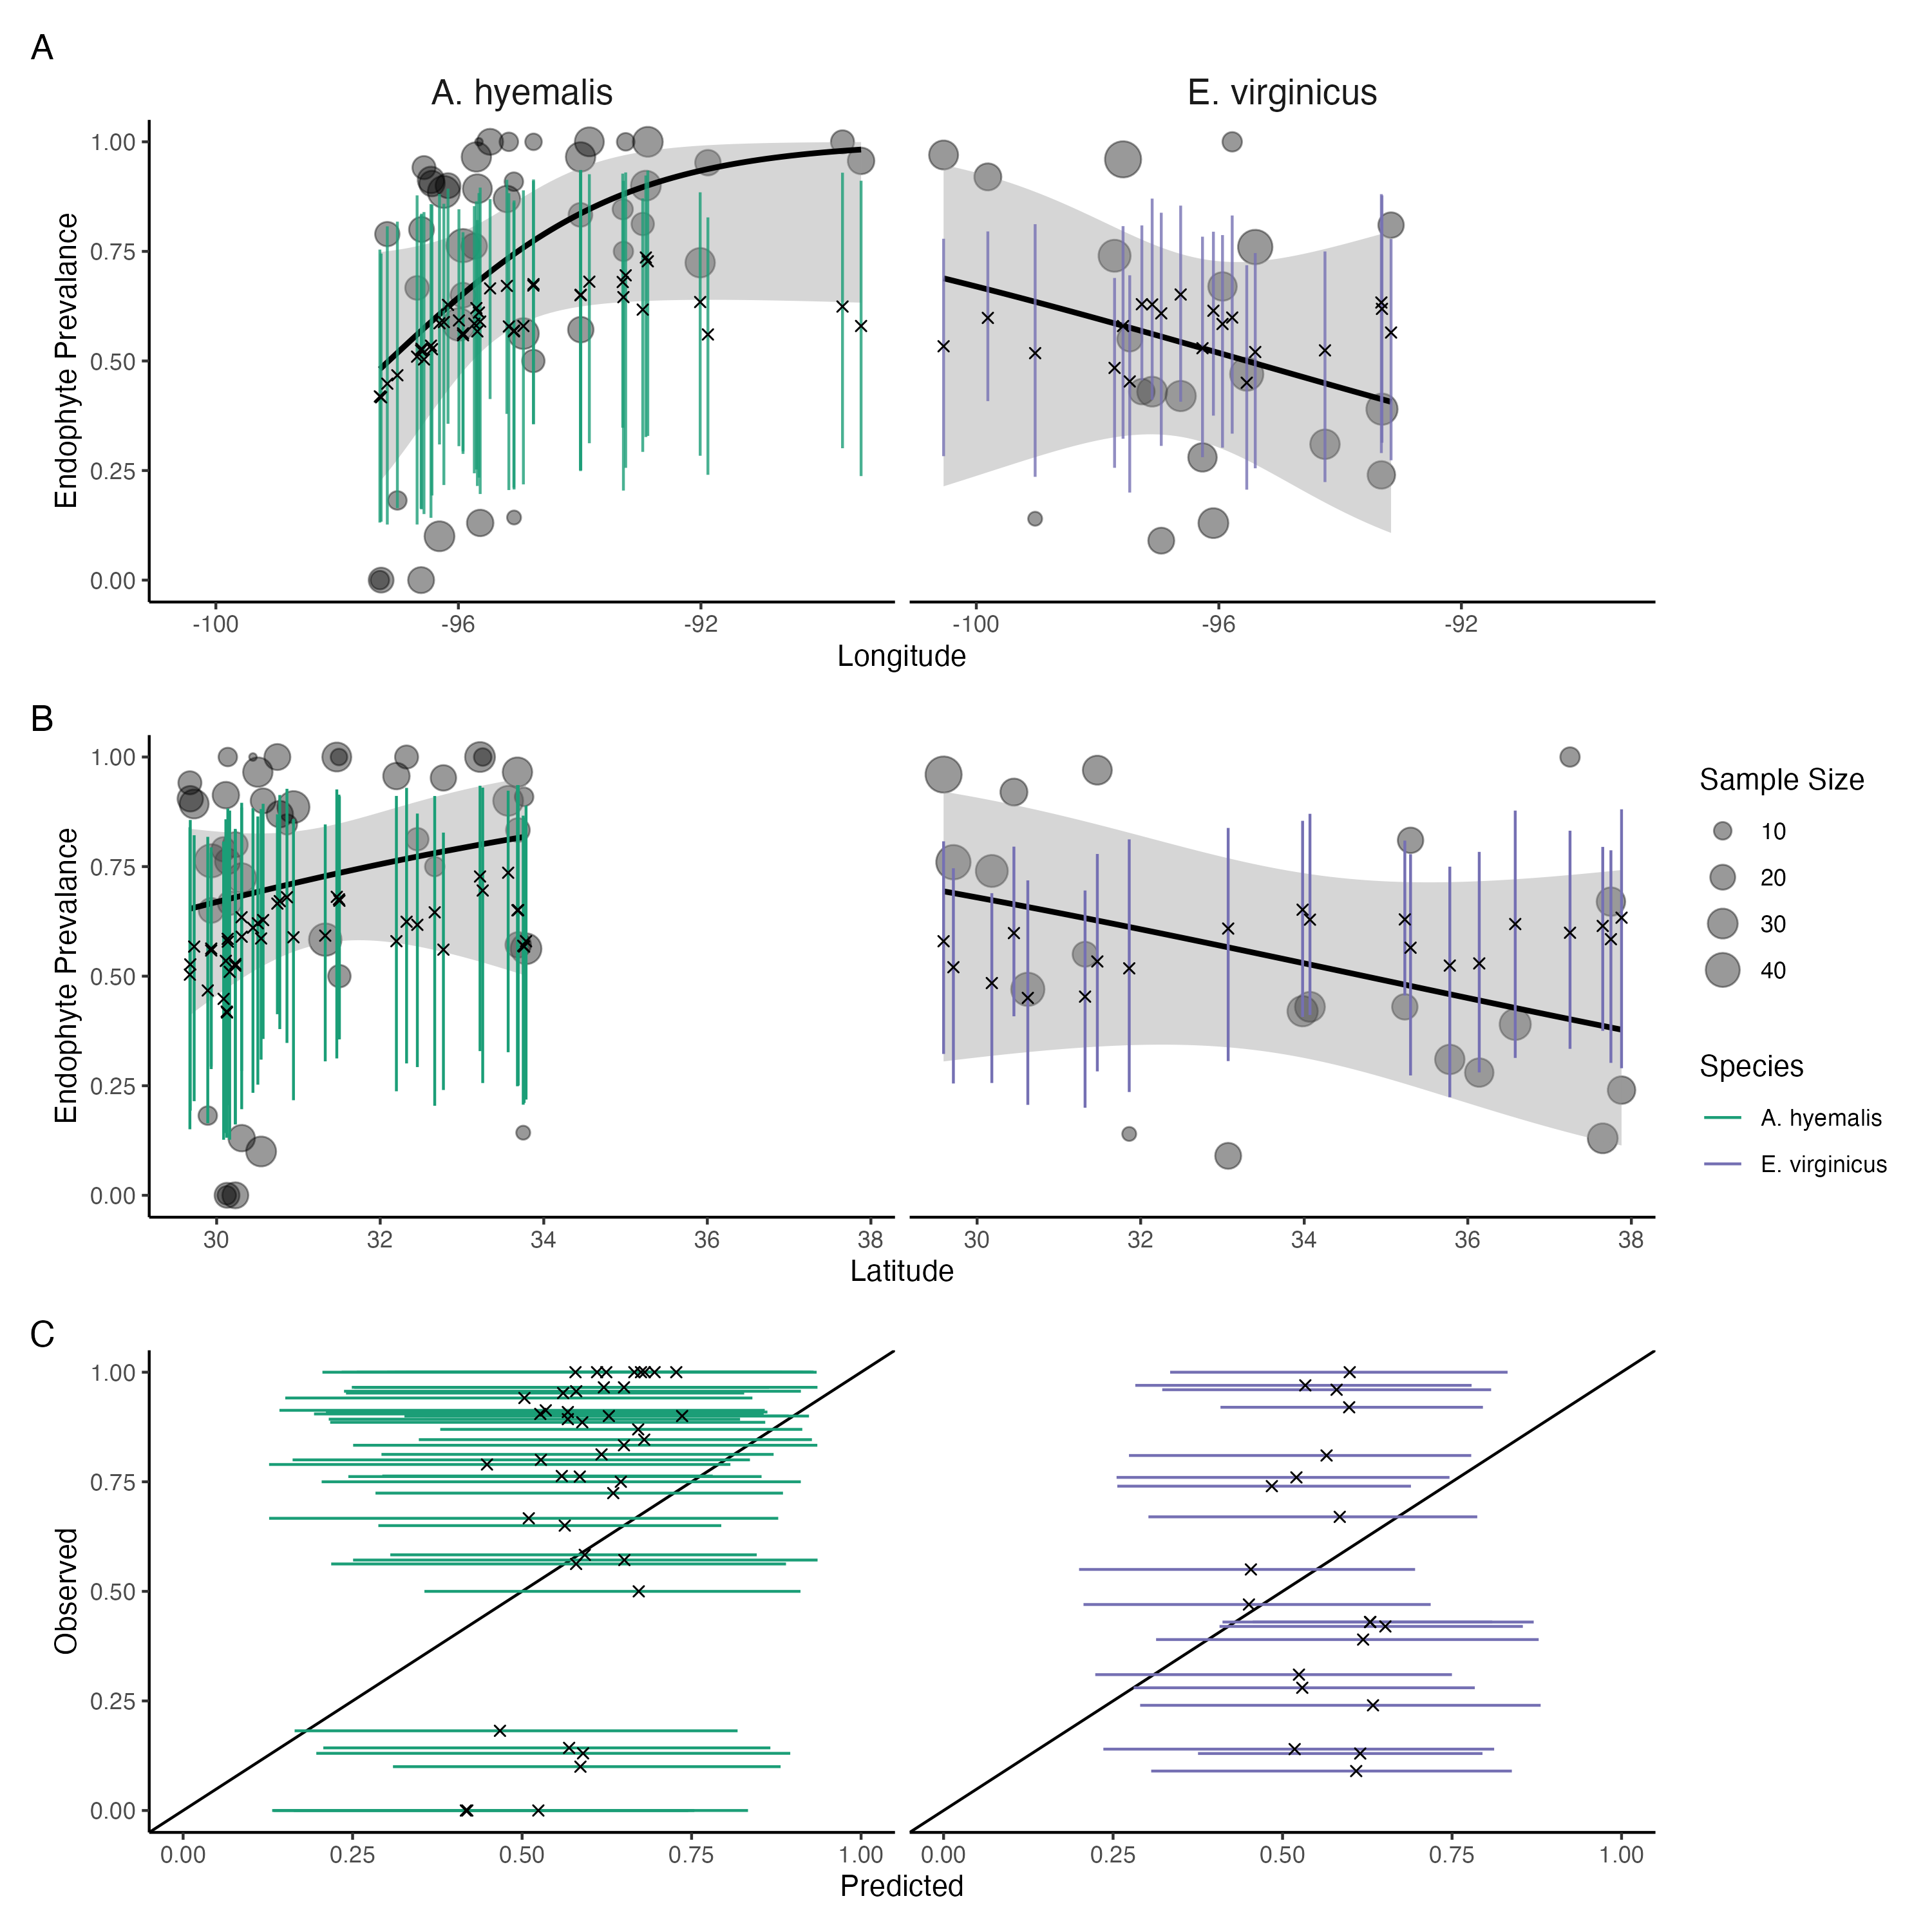
\includegraphics[width = \linewidth]{../Plots/contemp_test_plot.png}
	\caption{\textbf{Predicted vs observed endophyte prevalence for contemporary test data.} (A) The model, trained on historic herbarium collection data, performed modestly at predicting contemporary endophyte prevalence in \emph{A. hyemalis}, as indicated by some overlap of predicted 95\% CI with the 1:1 line, however contemporary test data generally had more variance between populations than model predictions. The model did recapitulate broader regional trends across (B) longitude and (C) latitude. Point size in panels B and C reflect sample sizes of contemporary endophyte population surveys.}
	\label{fig:contemptestplot}
\end{figure}

\subsection*{Assessing collector and scorer influences on predicted endophyte prevalence}
Our modeling effort quantified temporal and spatial trends in endophyte prevalence while accounting for potential biases introduced by collectors and by individual scorers who quantified endophyte presence/absence within specimens with the use of random effects. 
We found no evidence that collector biases influenced our results. 
Collector random effects were consistently small (Fig. \ref{fig:collector_fx}), and models fit with and without this random effect provide qualitatively similar results.
The identity of individual scorers did contribute to observed patterns in endophyte prevalence.
For example, $3$ of the $25$ scorers were more consistently likely than average to assign positive endophyte status, as indicated by 95\% credible intervals greater than zero) (Fig. \ref{fig:scorer_fx}). 
This may have been driven by differences in scorers biases during the seed scoring process or by unintended spatial clustering of the specimens scored by each scorer \cite{clayton1993spatial,urdangarin2023evaluating}. 
Interpreting our models with the inclusion of variance associated with the scorer effect thus provides conservative estimates of the absolute magnitude of changes in endophyte prevalence.



\section*{Discussion}
Our examination of historic plant specimens revealed a cryptic biotic reponse to climate change. 
For the three host species we examined, there have been clear increases in fungal endophyte prevalence over the last two centuries.
Increases in prevalence of \emph{Epichloë}, which are vertically transmitted, can potentially be interpreted as adaptive changes that improve the fitness of their hosts under stressful conditions.
This interpretation is in line with theory predicting that the positive fitness feedback caused by vertical transmission leads beneficial symbionts to rise in prevalence within a population \cite{fine1975vectors}.
We found that trends in endophyte prevalence varied across the distribution of each species in assocation with observed changes in climate drivers, suggesting that the endophytes have contributed to host resilience under environmental change.
Taken together, this suggests a strengthening of the mutualism over the last two centuries.


Differences between the responses of each host species underscore that while all of these $C_3$ grasses share similar broad-scale distributions, each engages in unique biotic interactions and has unique niche requirements.
We identified hotspots of change for \emph{A. perennans}, which experienced the strongest absolute changes in endophyte prevalence (Fig. \ref{fig:svc_time_map}).
Declines in the southern portion of its range and increases in the north suggest a potential poleward range shift of endophytic plants. 
Based on previous work demonstrating that endophytes can shield their hosts from drought stress \cite{decunta2021systematic}, we generally predicted that drought conditions could be a driver of increasing endophyte prevalence. 
In contrast to this expectation, increasing prevalence for this species was associated with increasing autumn temperature and precipitation (Fig. \ref{fig:climate_correlation_plot}). 
To our knowledge, the response of the symbiosis in \emph{A. perennans} to drought has not been examined experimentally, but in a greenhouse experiment, endophytes had a positive effect on host reproduction under shaded, low-light conditions \citep{davitt2010costs}. 
Our results also hint that it may be useful to investigate whether lagged climate effects are important predictors of host fitness in this system \cite{evers2021lagged}.
Endophyte prevalence of the spring-flowering \emph{A. hyemalis} was most strongly linked to increasing variability in precipitation across summer and autumn.  
Endophytes could be playing a role helping hosts weather autumn-season droughts while the species is dormant.
Previous work has demonstrating drought benefits in a greenhouse manipulation with this species \citep{davitt2011understanding}, and early life stages may be particularly vulnerable to prolonged droughts.
%It is possible that the study region has not experienced a magnitude of climate change great enough to cause larger changes in endophyte prevalence for this species. 
%Weak associations with drought could also be explained by climate-driven changes in the rate of imperfect transmission (the generation of non-symbiotic offspring from symbiotic hosts), which could counterbalance endophyte-mediated fitness benefits \citep{donald2021context}. 
For \emph{E. virginicus}, which experienced the most modest changes in endophte prevalence overall, we only modest associations with changes in climate drivers. 
Surveys by \citet{sneck2017variation}, used as part of the test data in this study, identified a drought index (SPEI) that integrates precipitation with estimated evapotranspiration as an important predictor of endophyte prevalence.
\emph{Epichloë} endophytes have also been connected to a suite of non-drought related fitness benefits including herbivore protection \citep{brem2001epichloe}, salinity resistence \citep{wang2020effects}, and mediation of the soil microbiome \citep{roberts2015rhizosphere} 
These effects are potentially mediated by the diverse bioactive alkaloids and other signaling compounds they produce \citep{saikkonen2013chemical}.
Increases in symbionts could be explained, at least in part, by these diverse benefits that may help hosts weather a world made increasingly stressful by changes in climate and other anthropogenically introduced stressors.
While we show consistent increasing trends in prevalence between the three species, the mechanisms that explain these changes may be diverse and idiosyncratic. 

Our spatially-explicit model predicted regions of both high and low endophyte prevalence, suggesting that symbiotic and non-symbiotic host plants have overlapping, but non-identical niche requirements.
Endophytes fitness benefits potentially explain the spatial distribution of prevalence by allowing their hosts to persist in environments where they otherwise could not \citep{afkhami2014mutualist, kazenel2015mutualistic}.
For example, fitness benefits of the symbiosis could explain historically low prevalence in \emph{A. hyemalis} towards its western range edge coinciding with a strong aridity gradient.
Previous population surveys for endophytes, which were used as test data for our model, found similar regional trends in prevalence for endophyte host species \citep{sneck2017variation,rudgers2009benefits}. 
While the model recreated these large-scale spatial trends, test data contained more population-to-population variability in prevalence. 
Validating our model predictions in this way allows us to evaluate places to improve the model's out-of-sample predictive ability, which will be particularly important for predicting host and symbiont niche-shifts under future climate change.
Lack of information on local variability may simply be a feature of data derived from herbarium specimens. 
They are samples from local populations, but they are single specimens that are aggregated over in broad-scale model estimates.
Poor predictive ability at local scales in this grass-endophyte system is not surprising, as previous studies have found that local variation, even to the scale of hundreds of meters can structure endophyte-host niches \cite{kazenel2015mutualistic}. 
Other studies have found factors including land-use history \cite{vikuk2019infection} and the biotic environment, including herbivory \cite{rudgers2016long}, and host genotype \citet{sneck2017variation}, to be important predictors of endophyte ecology.
Incorporating available climatic and soil layers as covariates is an obvious first step that could improve predictions.
Another important step would be integrating data from local and regional scales  through modeling to constrain estimates of local and regional variation.
These steps will bridge gaps that often exist between large but broad bioclimatic and biodiversity data and small but local data on biotic interactions, and move towards the goal of predicting the dynamics of microbial symbioses under climate change \cite{miller2019recent, isaac2020data}.


Our analysis advances the use of herbarium specimens in global change biology in two ways. 
First and foremost, this is the first study to link long-term changes in microbial symbioses to changes in climate using specimens from natural history collections.
The responses of microbial symbioses are a rich target for future studies within museum specimens, particularly those that take advantage of advances in sequencing technology.
While we used relatively coarse presence/absence data based on fungal morphology, other studies have examined historic plant microbiomes using molecular sequencing and sophisticated bioinformatics techniques, but these studies have so far been limited to relatively few specimens at limited spatial extents \cite{yoshida2015computational,heberling2019utilizing, bieker2020metagenomic,gross2021hidden,bradshaw2021global}. 
Continued advances in capturing historic DNA and in filtering out potential contamination during specimen storage \citep{daru2019novel,bakker2020herbarium,raxworthy2021mining} will be imperative in the effort to scale up these efforts. 
This scaling up will be essential to be able to quantify changes not just in the prevalence of symbionts, but also in symbionts' intraspecific variation and evolutionary responses to climate change, as well as  in changes in the wider microbial community. 
Answering these questions as well as the unknown questions that future researchers may ask also reiterates the value in capturing meta-information during ongoing digitization efforts at herbaria around the world and during the accession of newly collected specimens \citep{lendemer2020extended,edwards2024university}.
Second, we accounted for several potential biases in the data observation process that may be common to many collections-based research questions by using a spatially-explicit random effects model. 
Spatial autocorrelation \cite{willems2022forest}, potential biases introduced by the sampling habits of collectors \citep{daru2018widespread}, and variation between contemporary researchers during the collection of trait data, if not corrected for could lead to over-confident inference about the strength and direction of historic change.
Previous studies that have quantified the effects of collector biases typically find them to be small  \cite{davis2015herbarium,meineke2019herbarium}, and we similarly did not find that collector has a strong effect on the results of our analysis.
%Fitting this model in a Bayesian framework allows for full propagation of uncertainty.

Ultimately, a central goal of global change biology is to generate predictive insights into the future of natural systems. 
While this survey of historic endophyte prevalence is necessarily correlative, it serves as a foundation to develop better predictive models of the response of microbial symbioses to climate change. 
Combining the insights from this type of regional-scale survey with field experiments and physiological data could be invaluable. 
While we found that climate is strongly correlated with endophytes' temporal responses, we do not know why trends in prevalence were weak in some areas or how endophytes would respond to more extreme changes in climate.
For example, transplanting symbiotic and non-symbiotic plants beyond the range edge of \emph{A. hyemalis} could tell us whether persistent low endophyte prevalence in that area is a result of environmental conditions that lead the symbiosis to negative fitness consequences, or is a result of some historical contingency or dispersal limitation that has thus far limited the presence of symbiotic hosts from a region where they would otherwise flourish and provide resilience.
While we observed evidence of mutualism resilience, more extreme environmental changes than those observed in our study could potentially push one or both partners beyond their physiological limit, leading to the collapse of the mutualism. 
Our analysis thus far is agnostic to changes in the distributions of hosts. 
Mechanistic models could connect the responses of both host and symbionts to abiotic climate drivers integrating dispersal processes. 
Beyond host-microbe symbioses, building these types of models would work towards quantitatively attributing biotic responses to anthropogenically driven climate change, similar to methods in climate science and economics \citep{stott2010detection, carleton2016social}.
%Elymus genotype
%Agrostis weedy



	%%%%%%%%%%%%%%%%%%%%%
	% Acknowledgments
	%%%%%%%%%%%%%%%%%%%%%
	% You may wish to remove the Acknowledgments section while your paper 
	% is under review (unless you wish to waive your anonymity under
	% double-blind review) if the Acknowledgments reveal your identity.
	% If you remove this section, you will need to add it back in to your
	% final files after acceptance.
	
	\section*{Acknowledgments}
	We thank Jessica Budke for help in drafting our initial destructive sampling plan, and to the many members of herbarium staff who facilitated our research visits, as well as to the hundreds of collectors who contributed to the natural history collections. 
	Several high schooler and undergraduate researchers contributed to data collection, including A. Appio-Riley, P. Bilderback, E. Chong, K. Dickens, L. Dufresne, B. Gutierrez, A. Johnson, S. Linder, E. Scales, B. Scherick, K. Schrader, E. Segal , G. Singla, and M. Tucker.
	This research was supported by funding from National Science Foundation (grants 1754468 and 2208857) and by funding from the Texas Ecolab Program.


	%%%%%%%%%%%%%%%%%%%%%
	% Statement of Authorship
	%%%%%%%%%%%%%%%%%%%%%
	% This section should also be commented out while your MS is undergoing
	% double-blind review. The specifics should of course be adapted to
	% your paper, but the paragraph below gives some hints of possible
	% contributions.
	
	\section*{Statement of Authorship}
J.C.F. contributed to research conception, data collection, data analysis, and led manuscript drafting.
J.M. contributed to data analysis and manuscript manuscript revisions.
T.E.X.M. contributed to research conception, data collection, data analysis, and manuscript revisions.

	
	\section*{Data and Code Availability}
	
	On initial submission, you may use this section to provide a URL for editors and reviewers that is `private for peer review'. After acceptance, this section must be updated with correct, working DOIs for data deposits (typically on the Dryad Digital Repository, ) and code deposits (such as in Zenodo). 
	
	\section*{Appendix A}
	\renewcommand{\thefigure}{A\arabic{figure}}
	\setcounter{figure}{0}
	
		\renewcommand{\thetable}{A\arabic{table}}
	\setcounter{equation}{0}  % reset counter 
	\setcounter{figure}{0}
	\setcounter{table}{0}
	
	\begin{figure}[H]
		\centering
		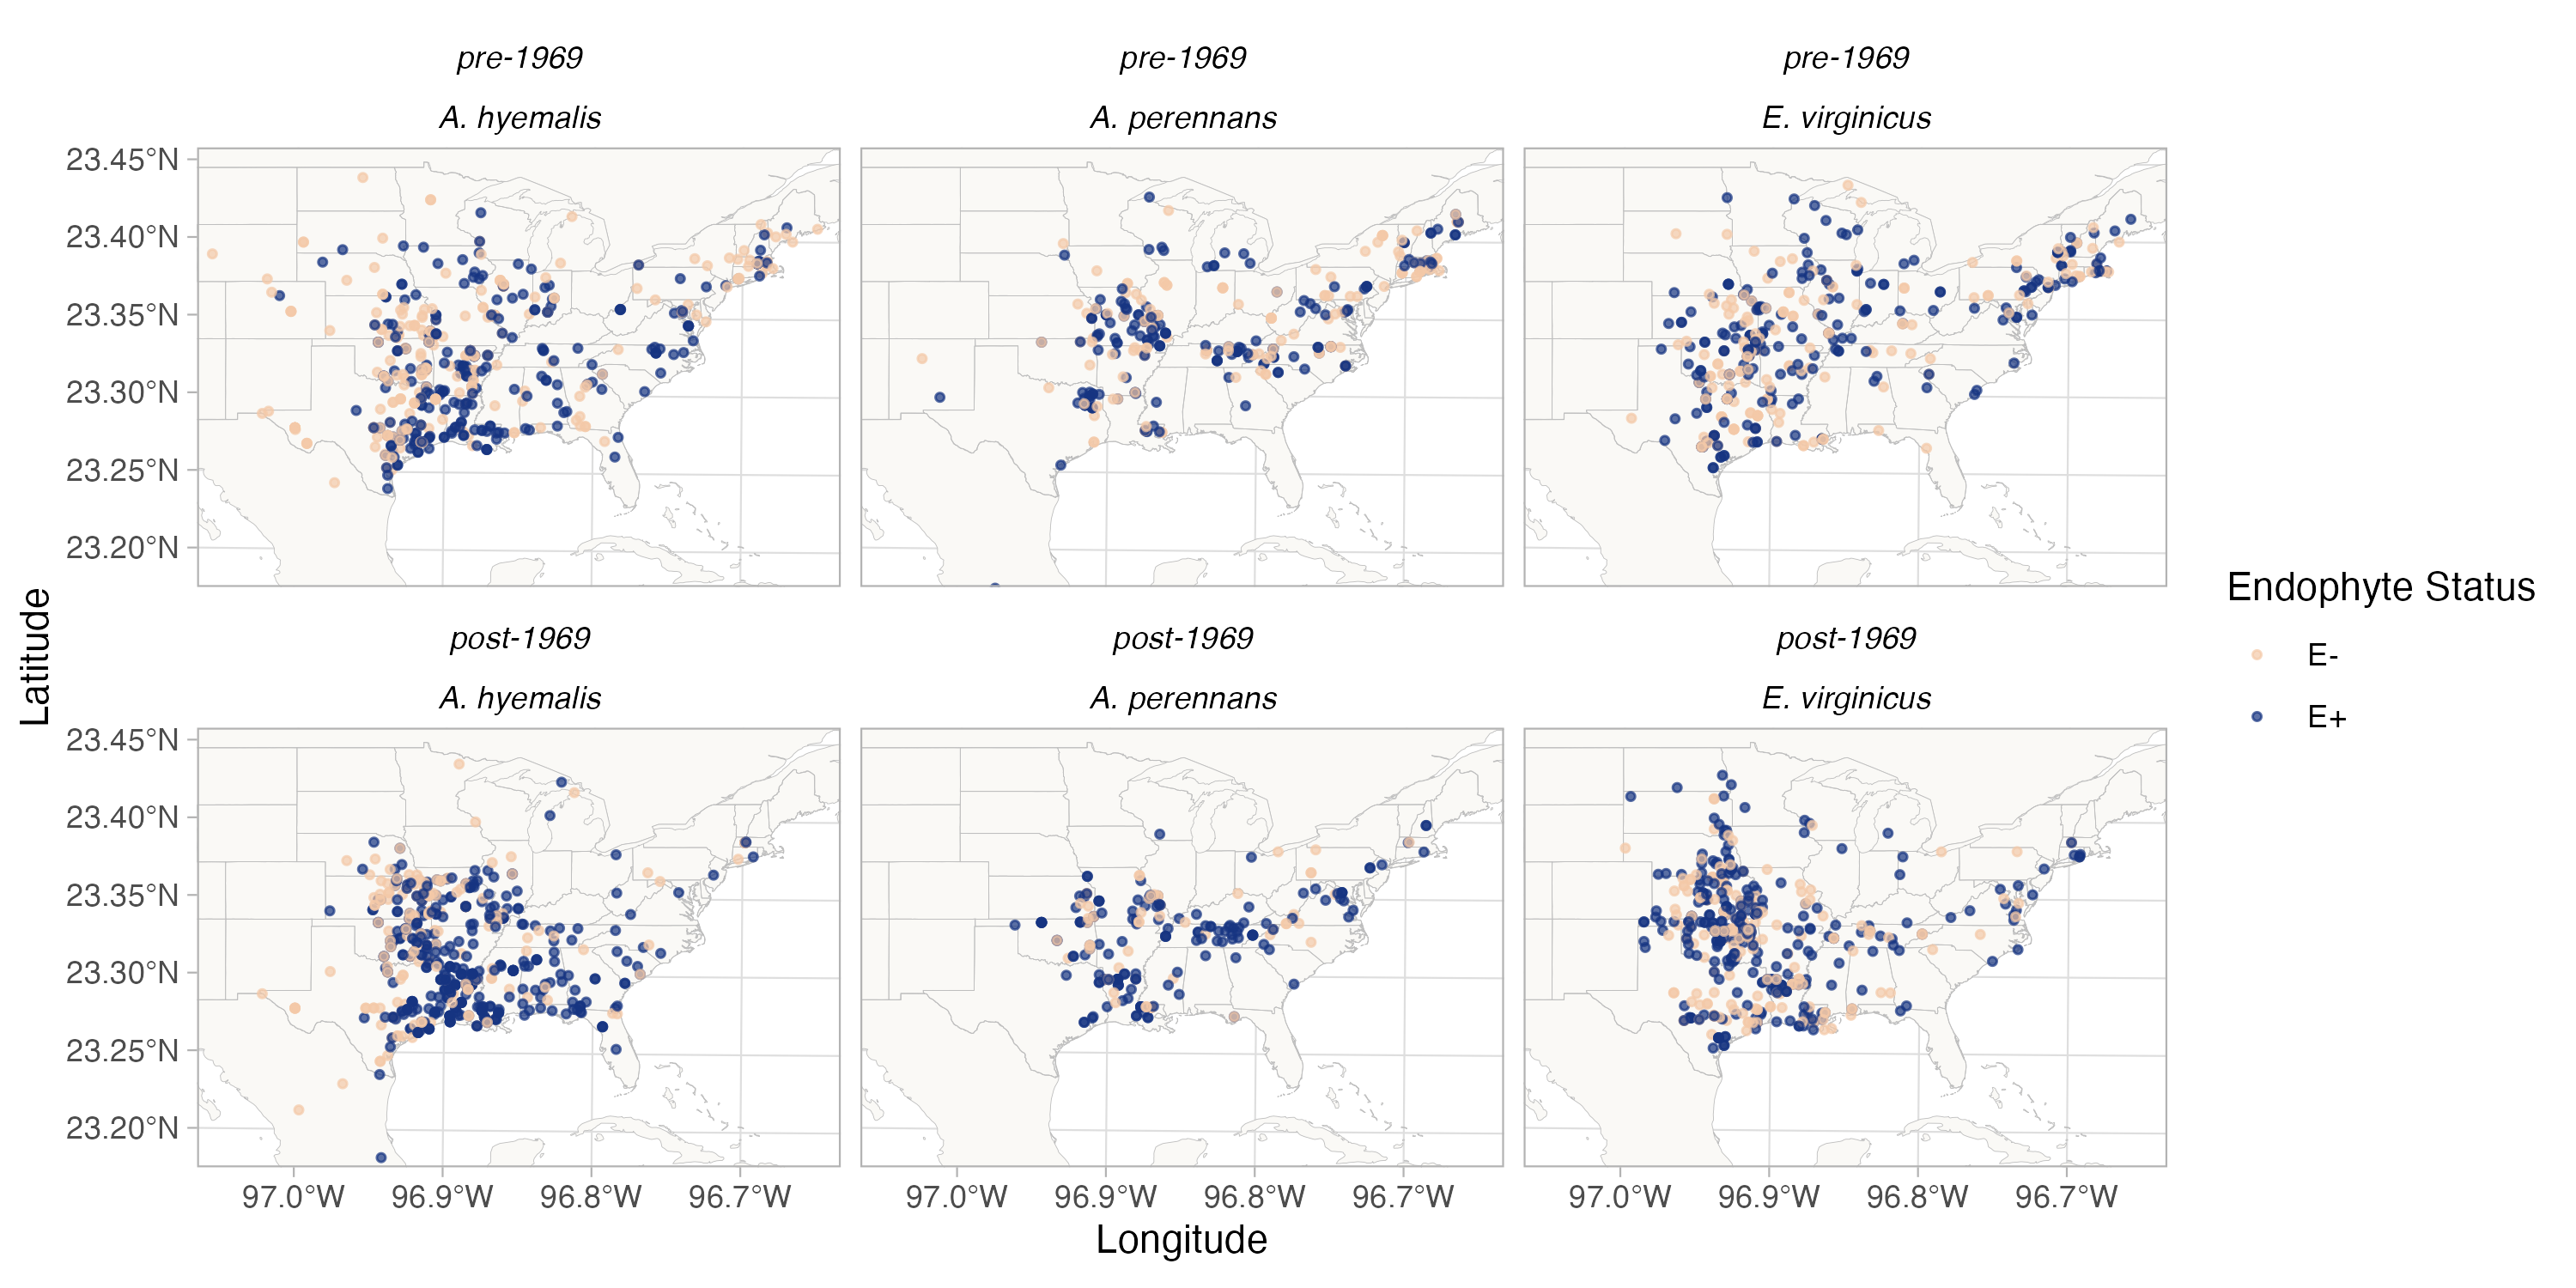
\includegraphics[width = \linewidth]{../Plots/endo_status_map.png}
		\caption{\textbf{Endophyte presence/absence in specimens of each host species.} Points show collection locations colored according to whether the specimen contained endophytes ( E+; blue points) or did not contain endophytes (E-, tan points) and are faceted based on collection period.}
		\label{fig:endo_status_map}
	\end{figure}
	
	\begin{figure}[H]
		\centering
		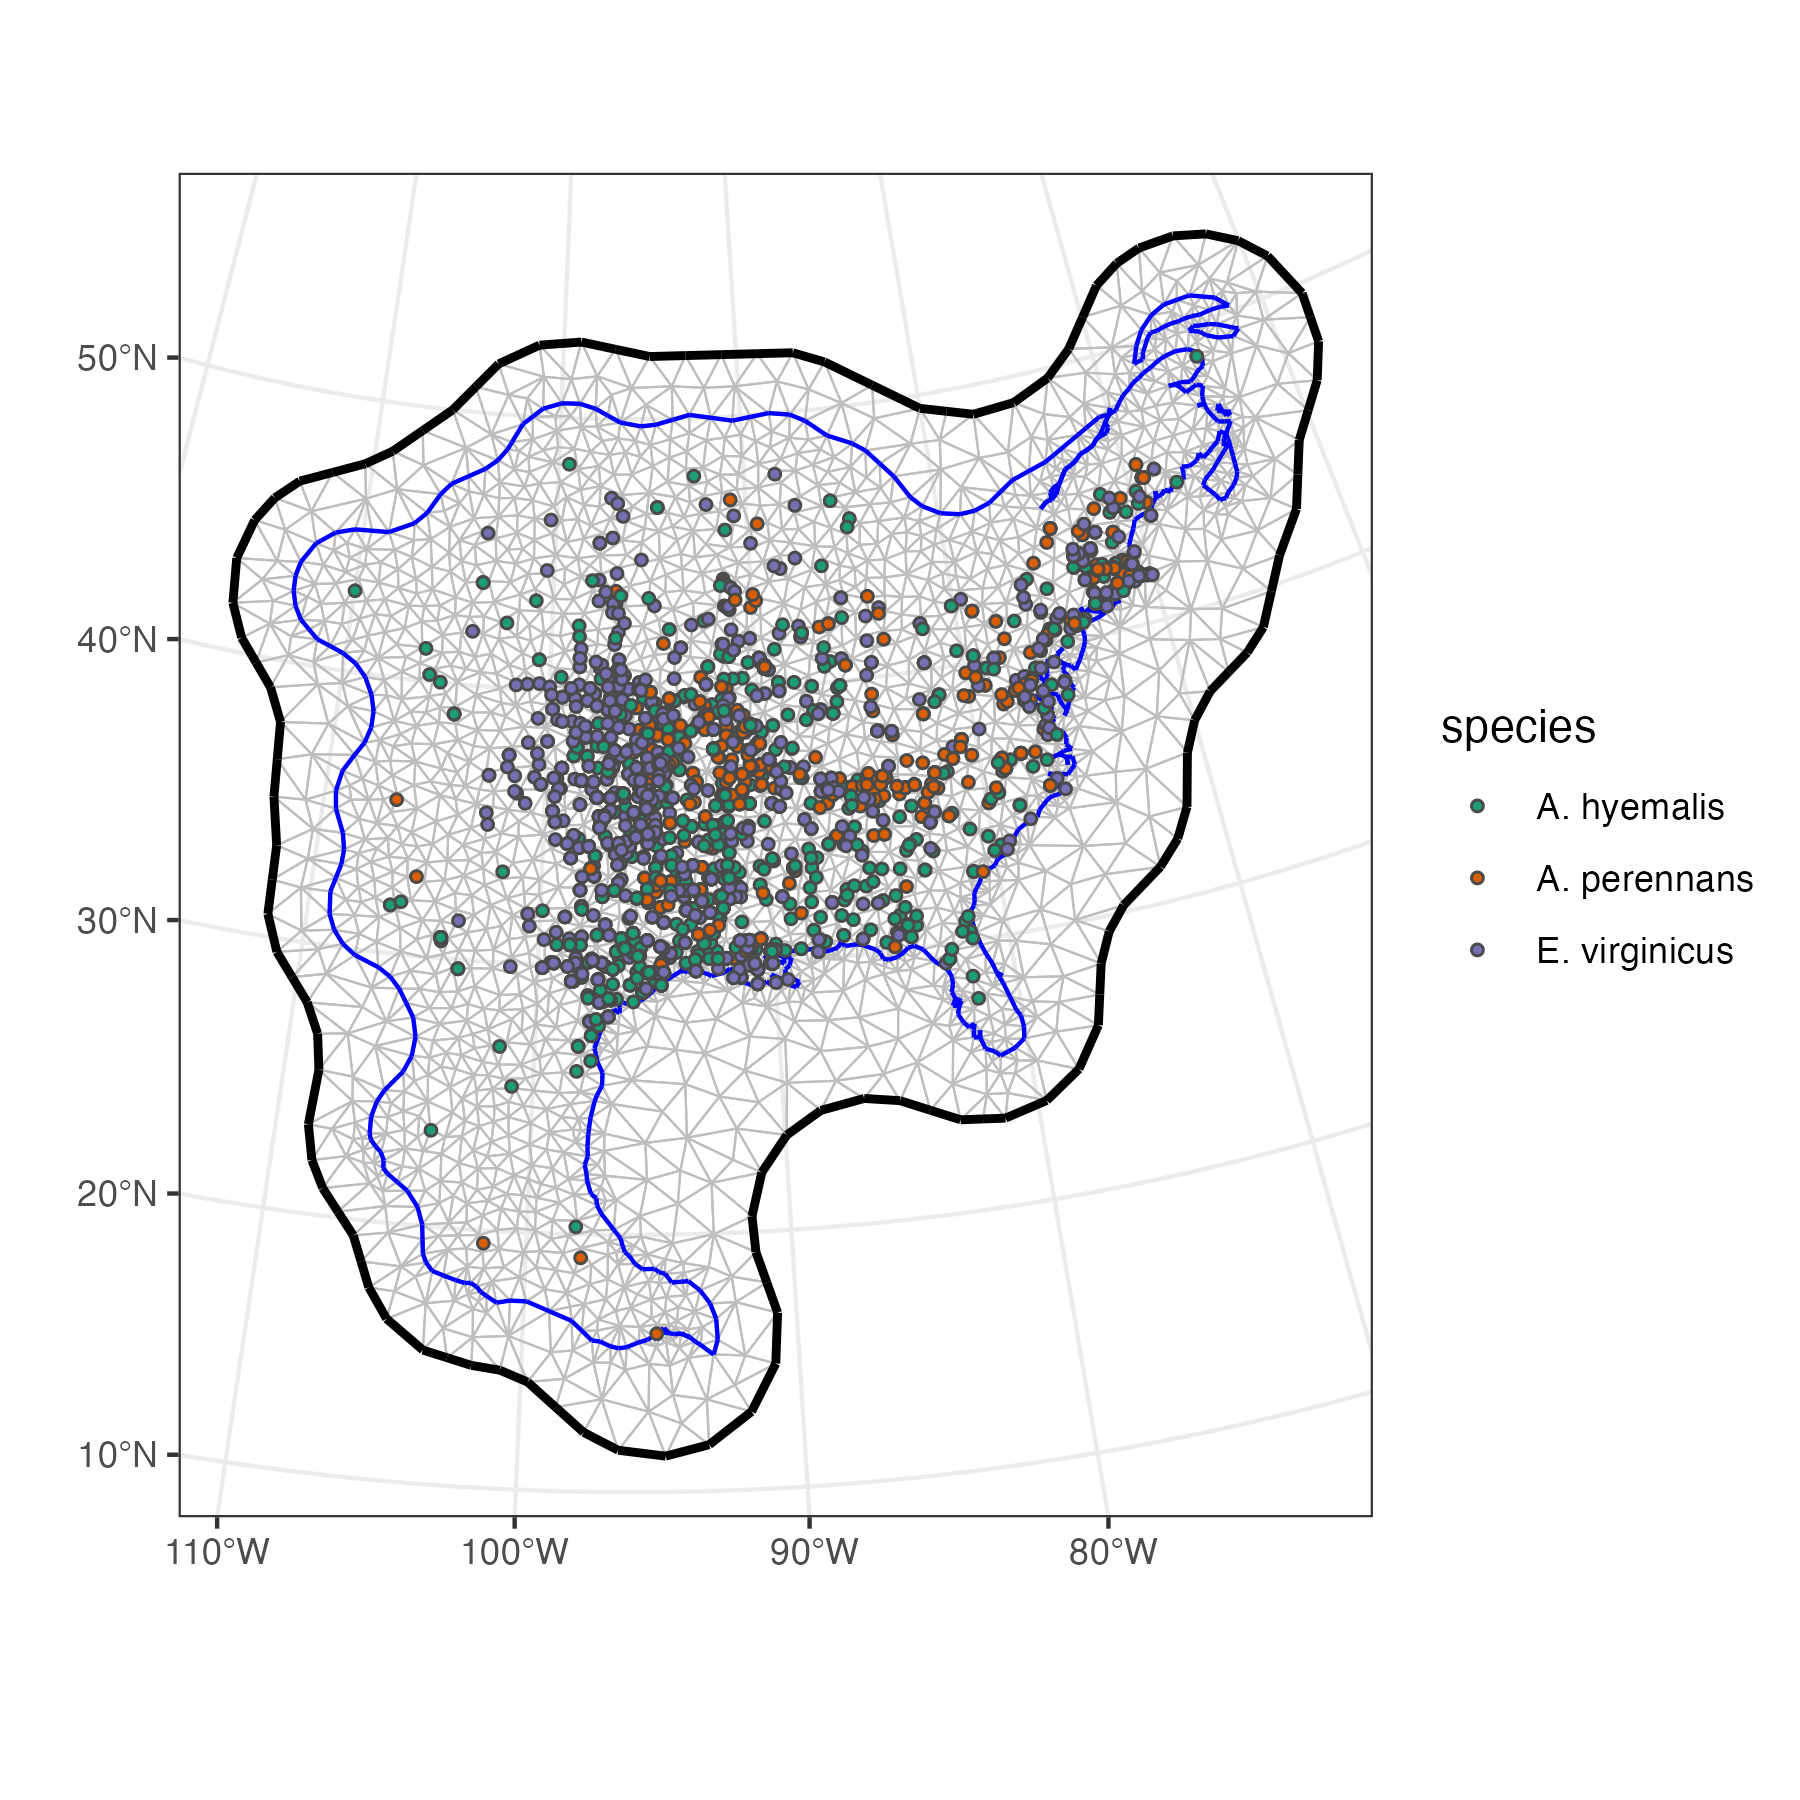
\includegraphics[width = \linewidth]{../Plots/mesh_plot.png}
		\caption{\textbf{Triangulation mesh used to estimate spatial dependence between data points}. Grey lines indicate edges of triangles used to define distances between observations. Colored points indicate locations of sampled herbarium specimens for each host species, and the blue line shows the convex hull and coastline used to define the edge of the mesh around the data points. The thick black line shows the convex hull defining a buffer space around the edge of the mesh to reduce the influence of edge effects on model estimates.}
		\label{fig:meshplot}
	\end{figure}

\begin{figure}[H]
	\centering
	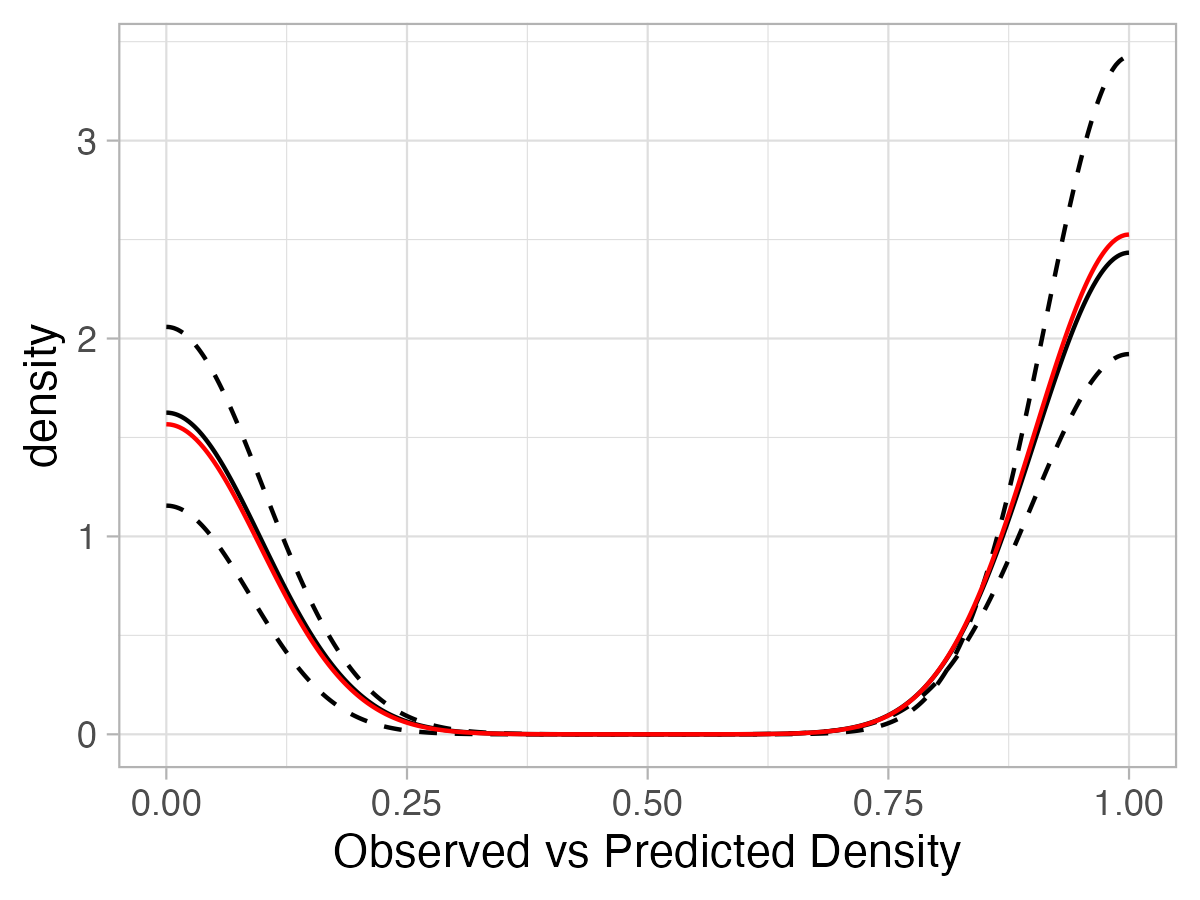
\includegraphics[width = .8\linewidth]{density_plot.png}
	\caption{\textbf{Consistency between real data and simulated values indicate that the fitted model accurately describes the data}. Graph shows density curves for the observed data (red) along with the mean(solid) and 95\% CI (dashed) of simulated values (black).}
\end{figure}

	
	\begin{figure}[H]
		\centering
		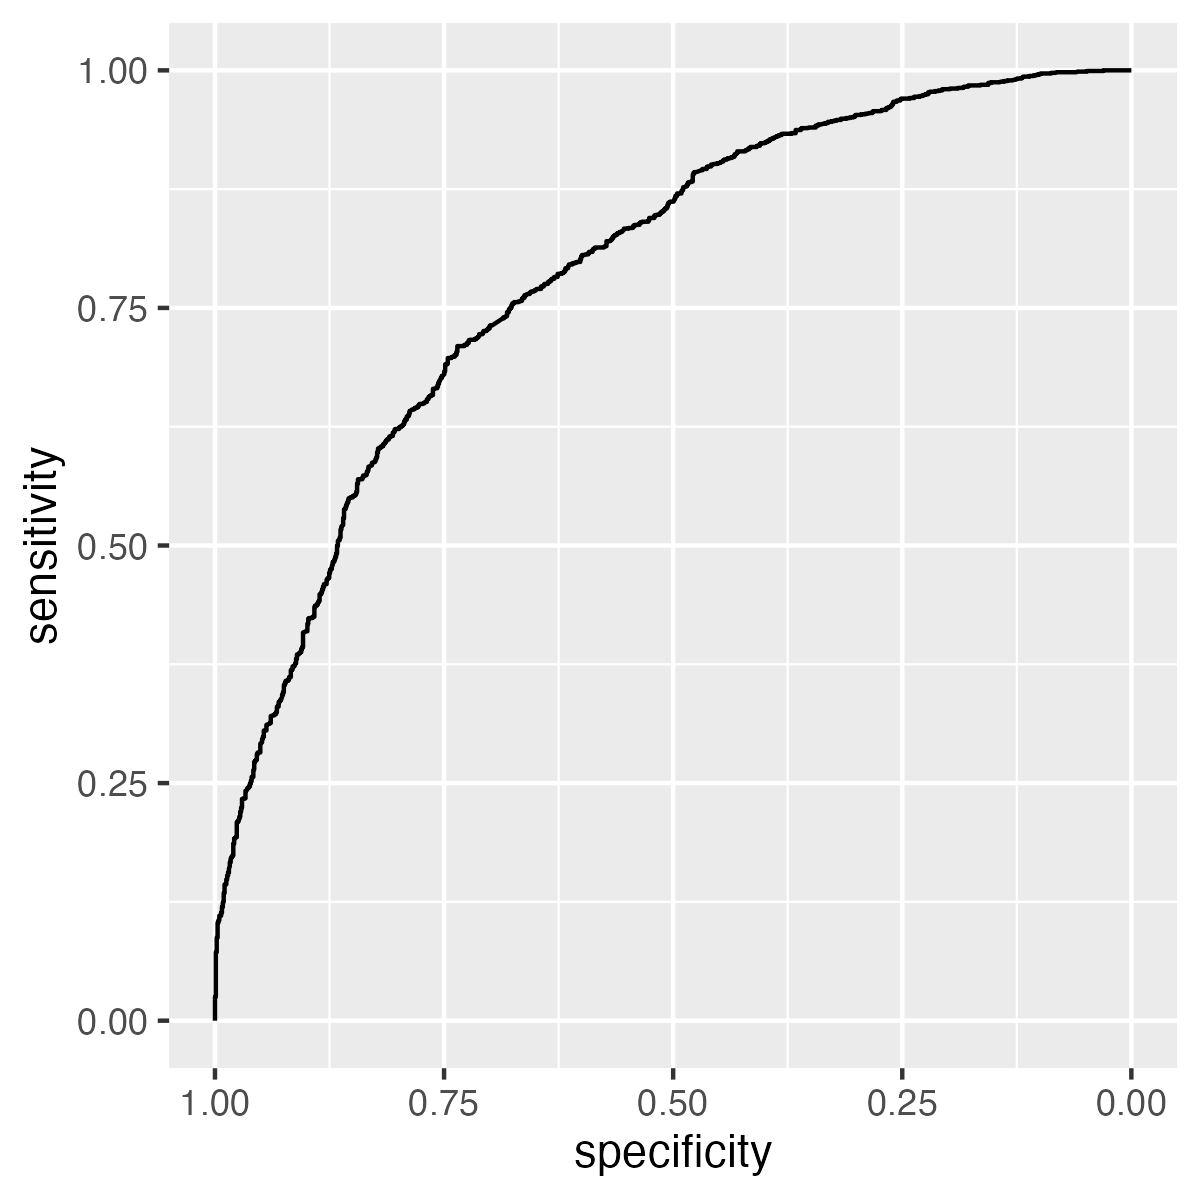
\includegraphics[width = .5\linewidth]{../Plots/ROC_training_plot.png}
		\caption{\textbf{ROC plot showing model performance classifying observations according to endophyte status within the in-sample data.} The curves show adequate model performance for observed data. The AUC value is 0.79.}
				\label{fig:ROCtraining}
	\end{figure}
	
		
	\begin{figure}[H]
		\centering
		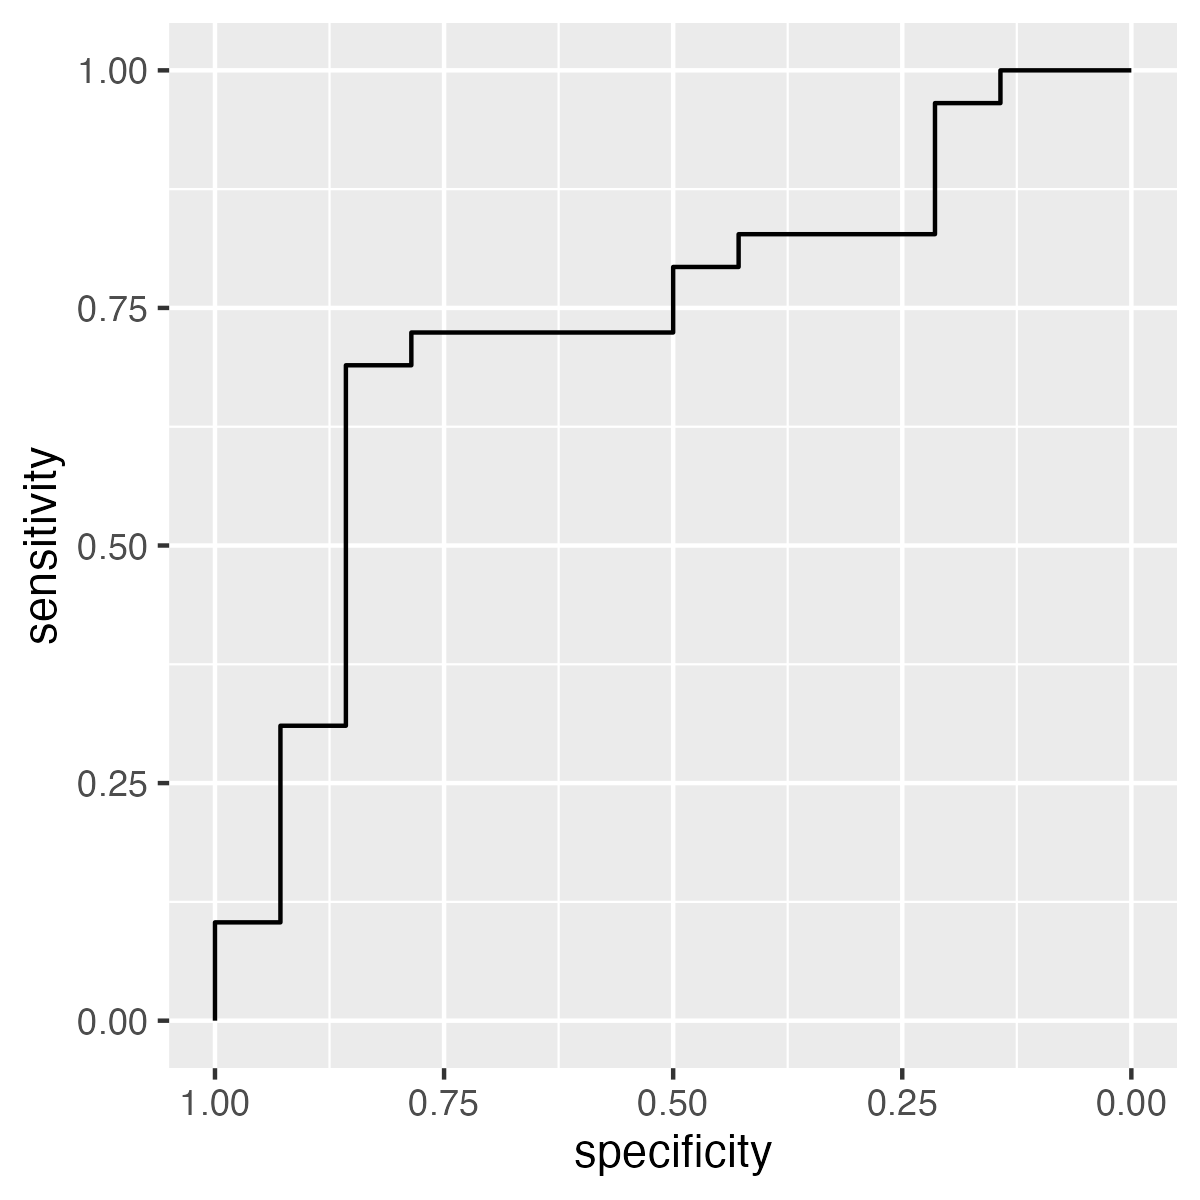
\includegraphics[width = .5\linewidth]{../Plots/ROC_test_plot.png}
		\caption{\textbf{ROC plot showing model performance classifying observations according to endophyte status within the out-of-sample data.} The curves show adequate model performance for test data. The AUC value is 0.77.}
		\label{fig:ROCtest}
	\end{figure}
	
	
\begin{figure}[H]
	\centering
	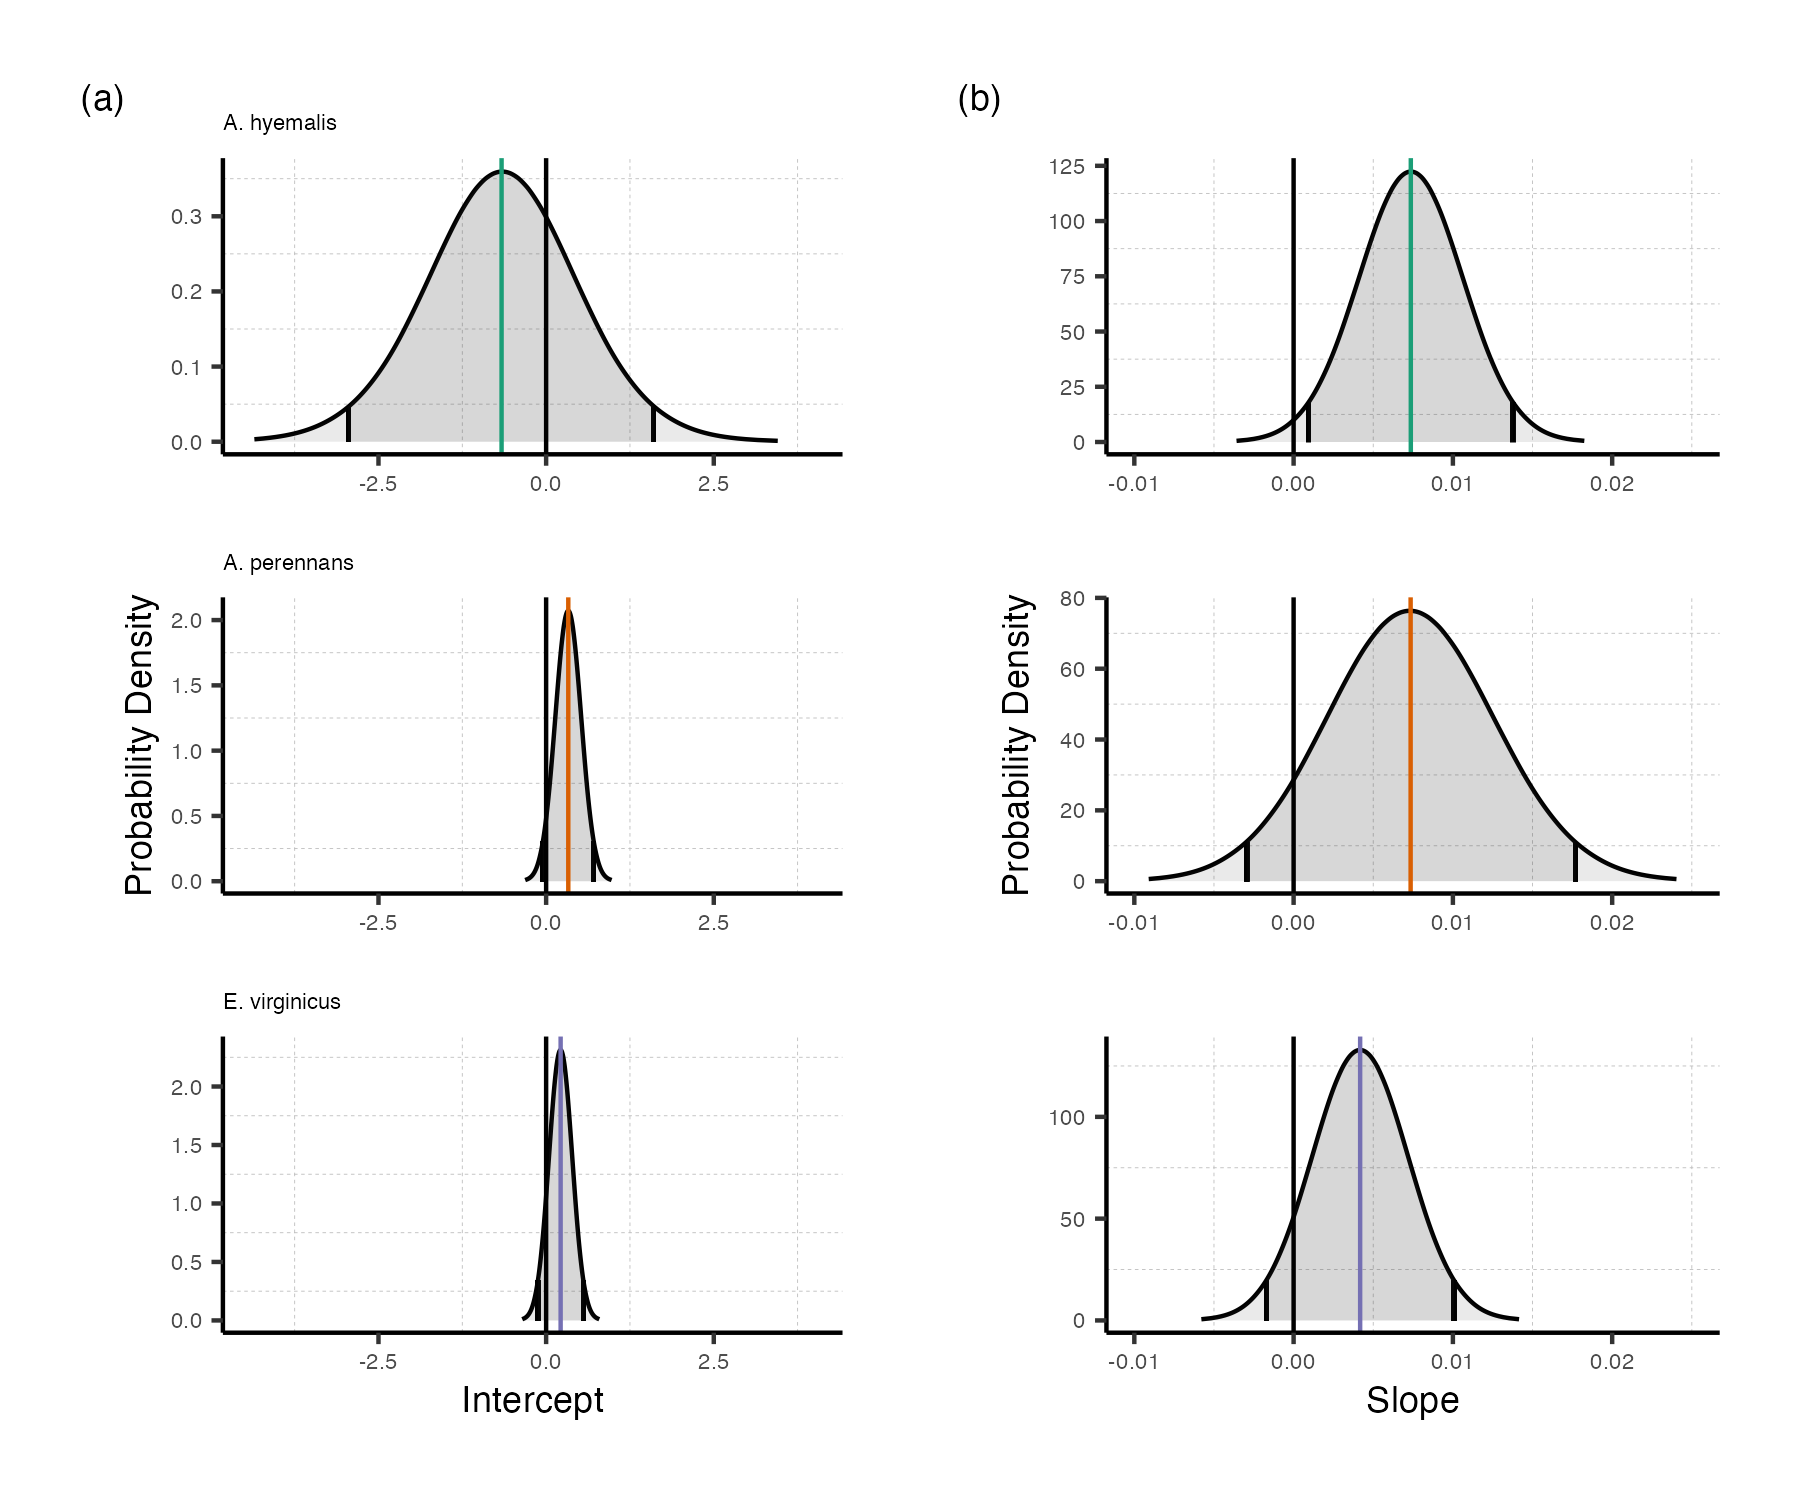
\includegraphics[width = \linewidth]{../Plots/posterior_plot.png}
	\caption[Posterior estimates of parameters describing global temporal trends in endophyte prevalence trends.]{Density curves show the probability density along with mean (colored line) and $95$\% CI (black lines) for the (A) intercept and (B) slope terms, \textbf{A} and \textbf{T} respectively. Colors represent each host species}
	\label{fig:temporal_posterior}
\end{figure}


\begin{figure}[H]
	\centering
	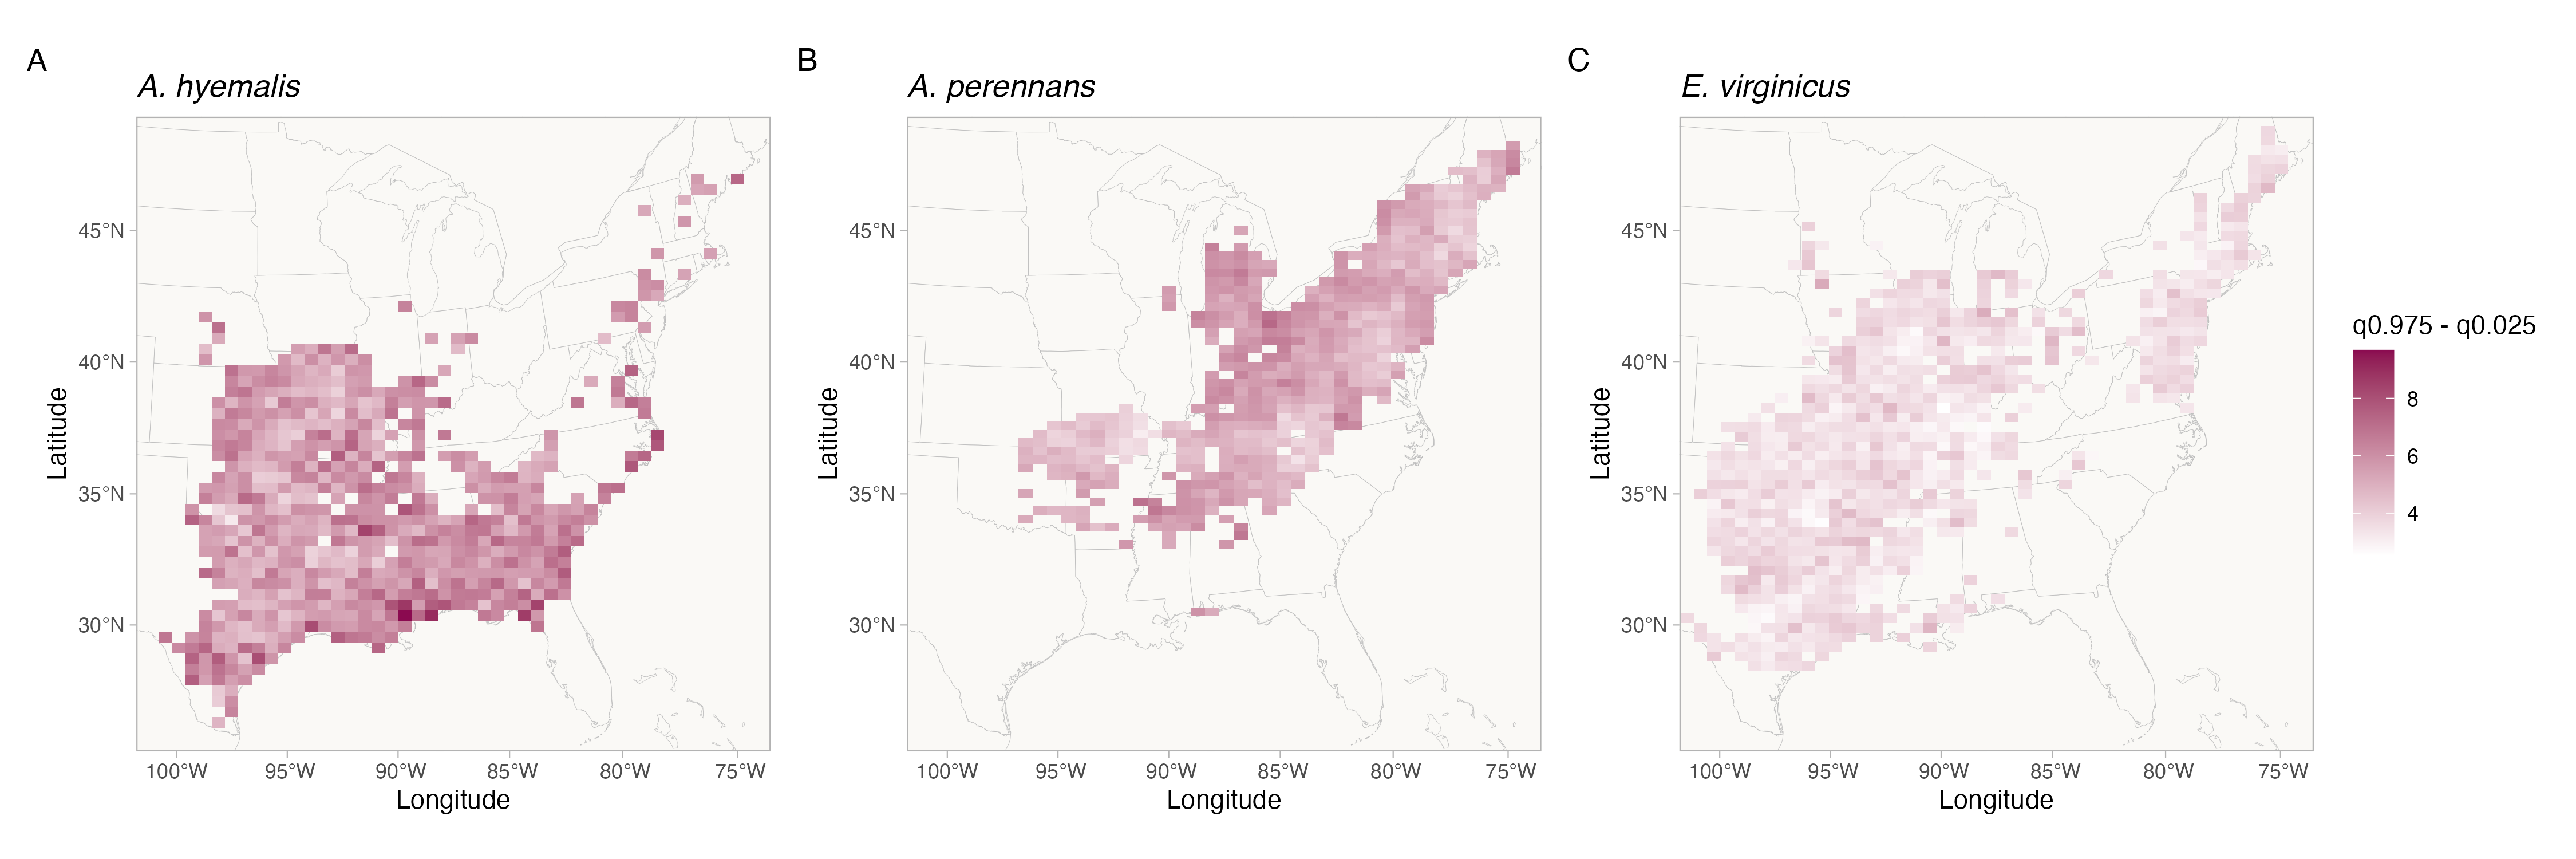
\includegraphics[width = \linewidth]{../Plots/svc_time_map_CI.png}
	\caption[Uncertainty in spatially-varying trends representing change in endophyte prevalence for each host species.]{Shading represents the range of the 95\% posterior credible interval for spatially varying slopes, $\tau$.}
	\label{fig:svc_time_map_CI}
\end{figure}


\begin{figure}[H]
	\centering
	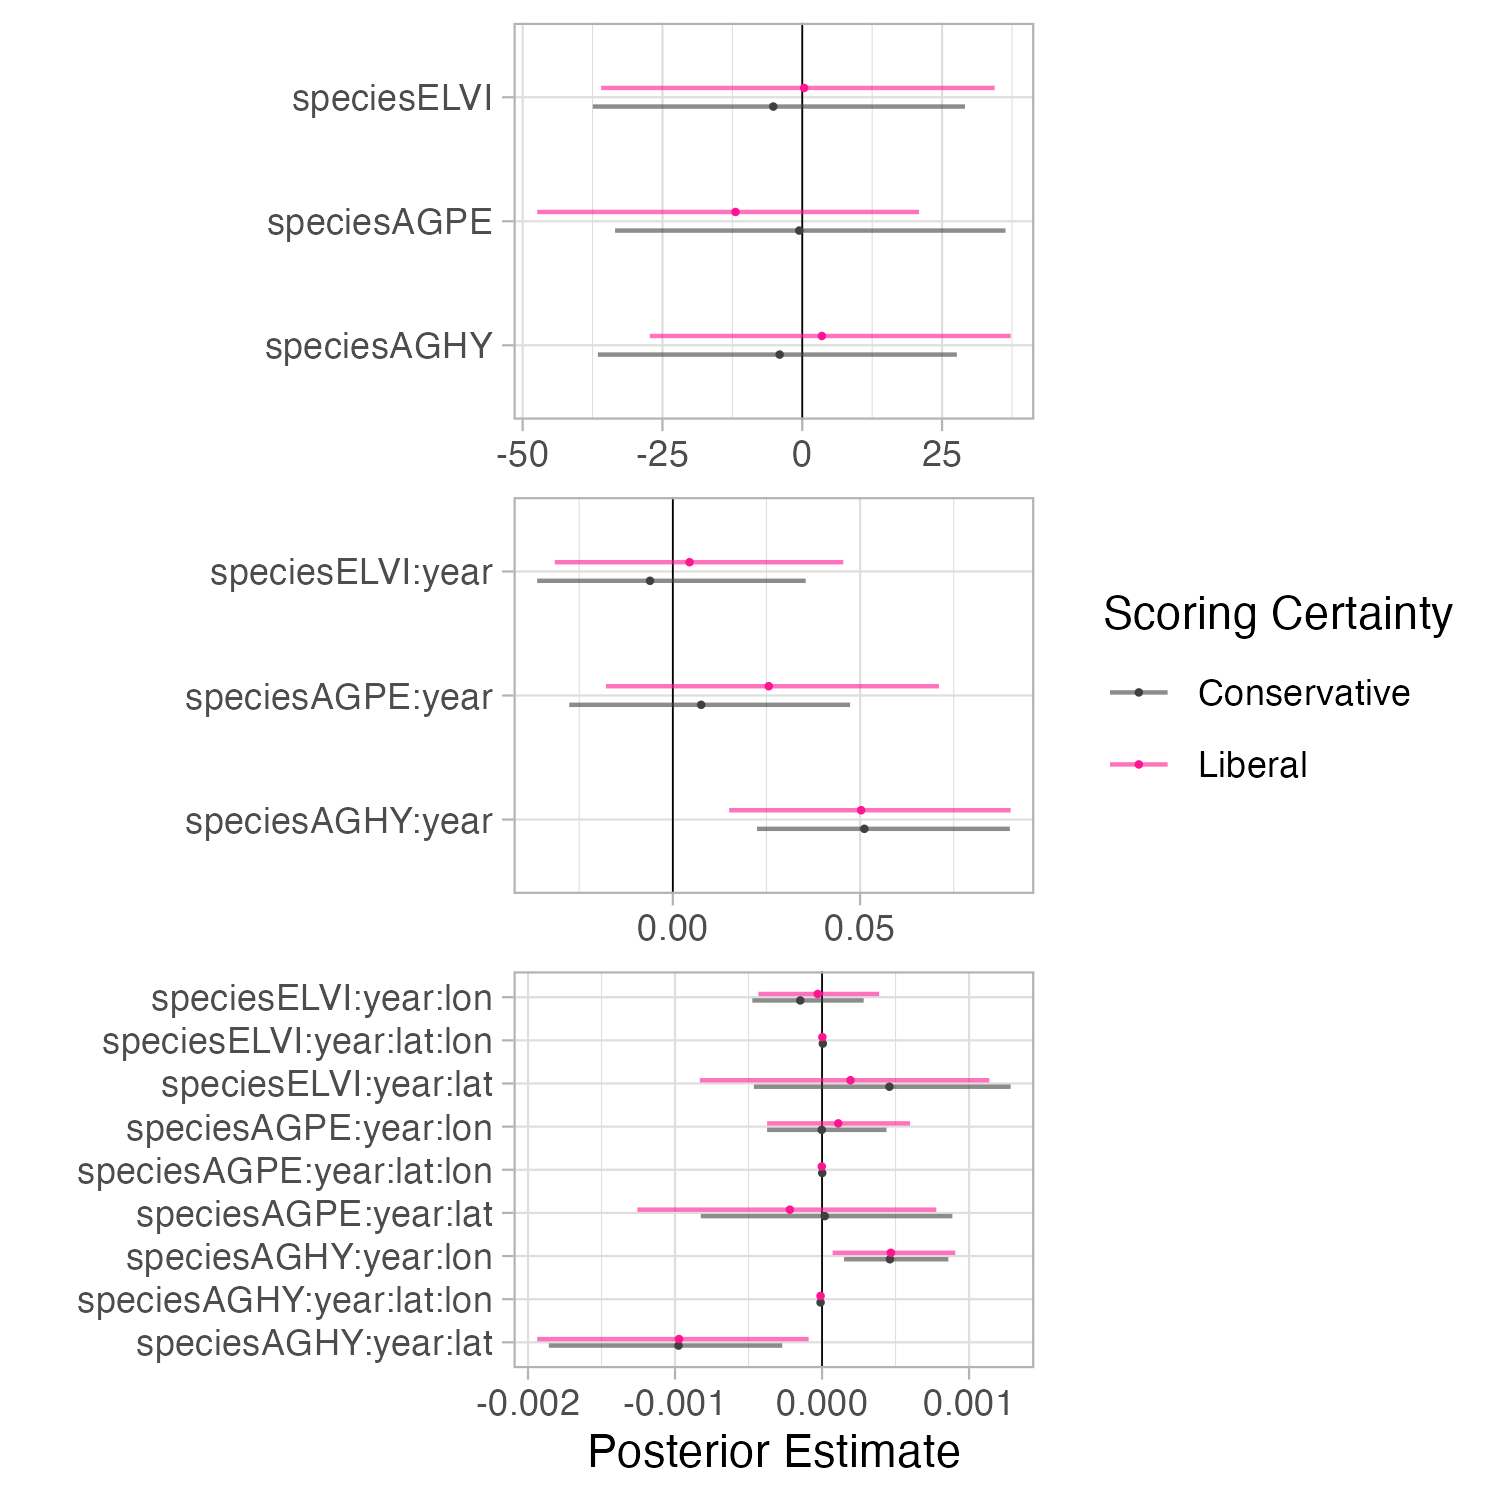
\includegraphics[width = \linewidth]{fixed_plot.png}
	\caption{\textbf{Comparison of posterior estimates of fixed effects when using Liberal or Conservative endophyte scores.}}
\end{figure}


\begin{figure}[H]
	\centering
	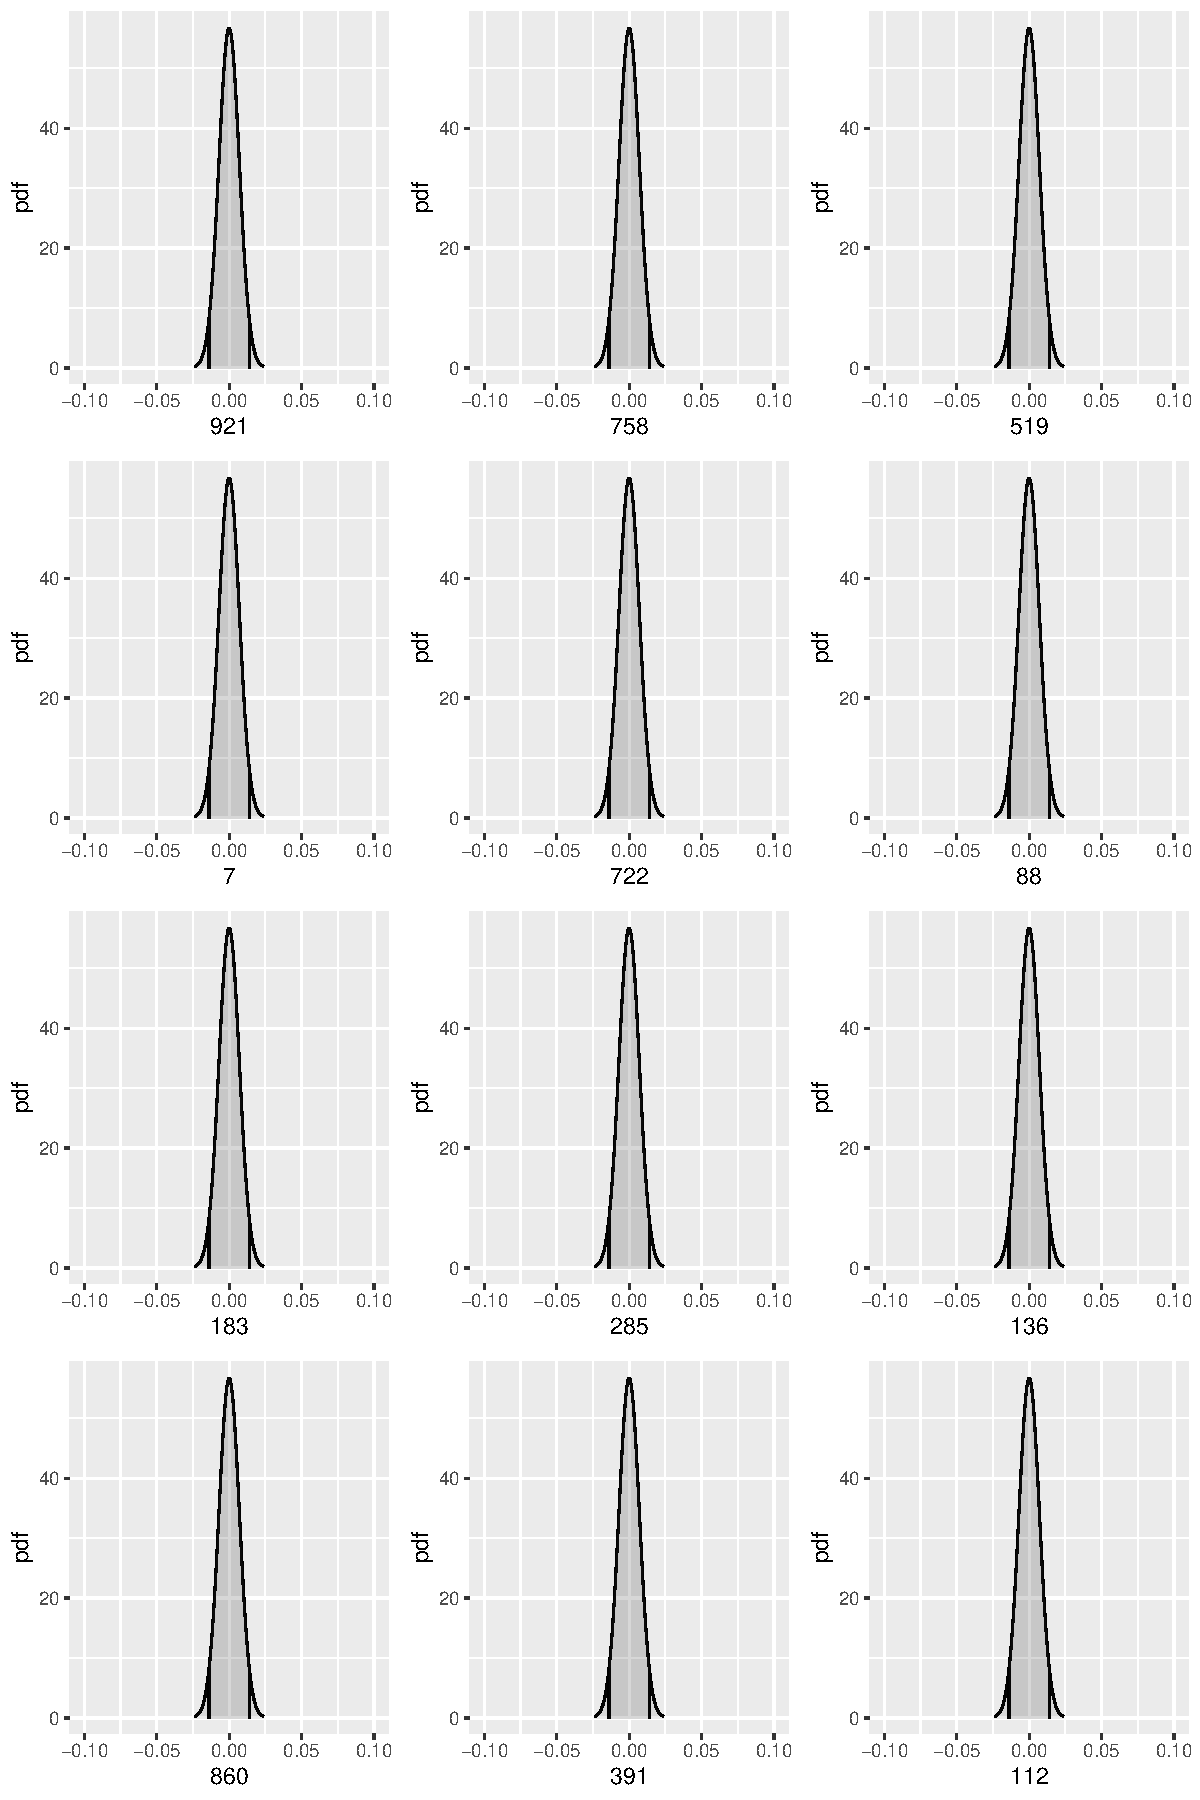
\includegraphics[width = .8\linewidth]{../Plots/collector_posterior_plot.pdf}
	\caption{\textbf{Posterior estimates of collector random effects.} Density curves show the posterior estimate along lines indicating the 95\% CI for 12 randomly selected collectors.}
		\label{fig:collector_fx}
\end{figure}


\begin{figure}[H]
	\centering
	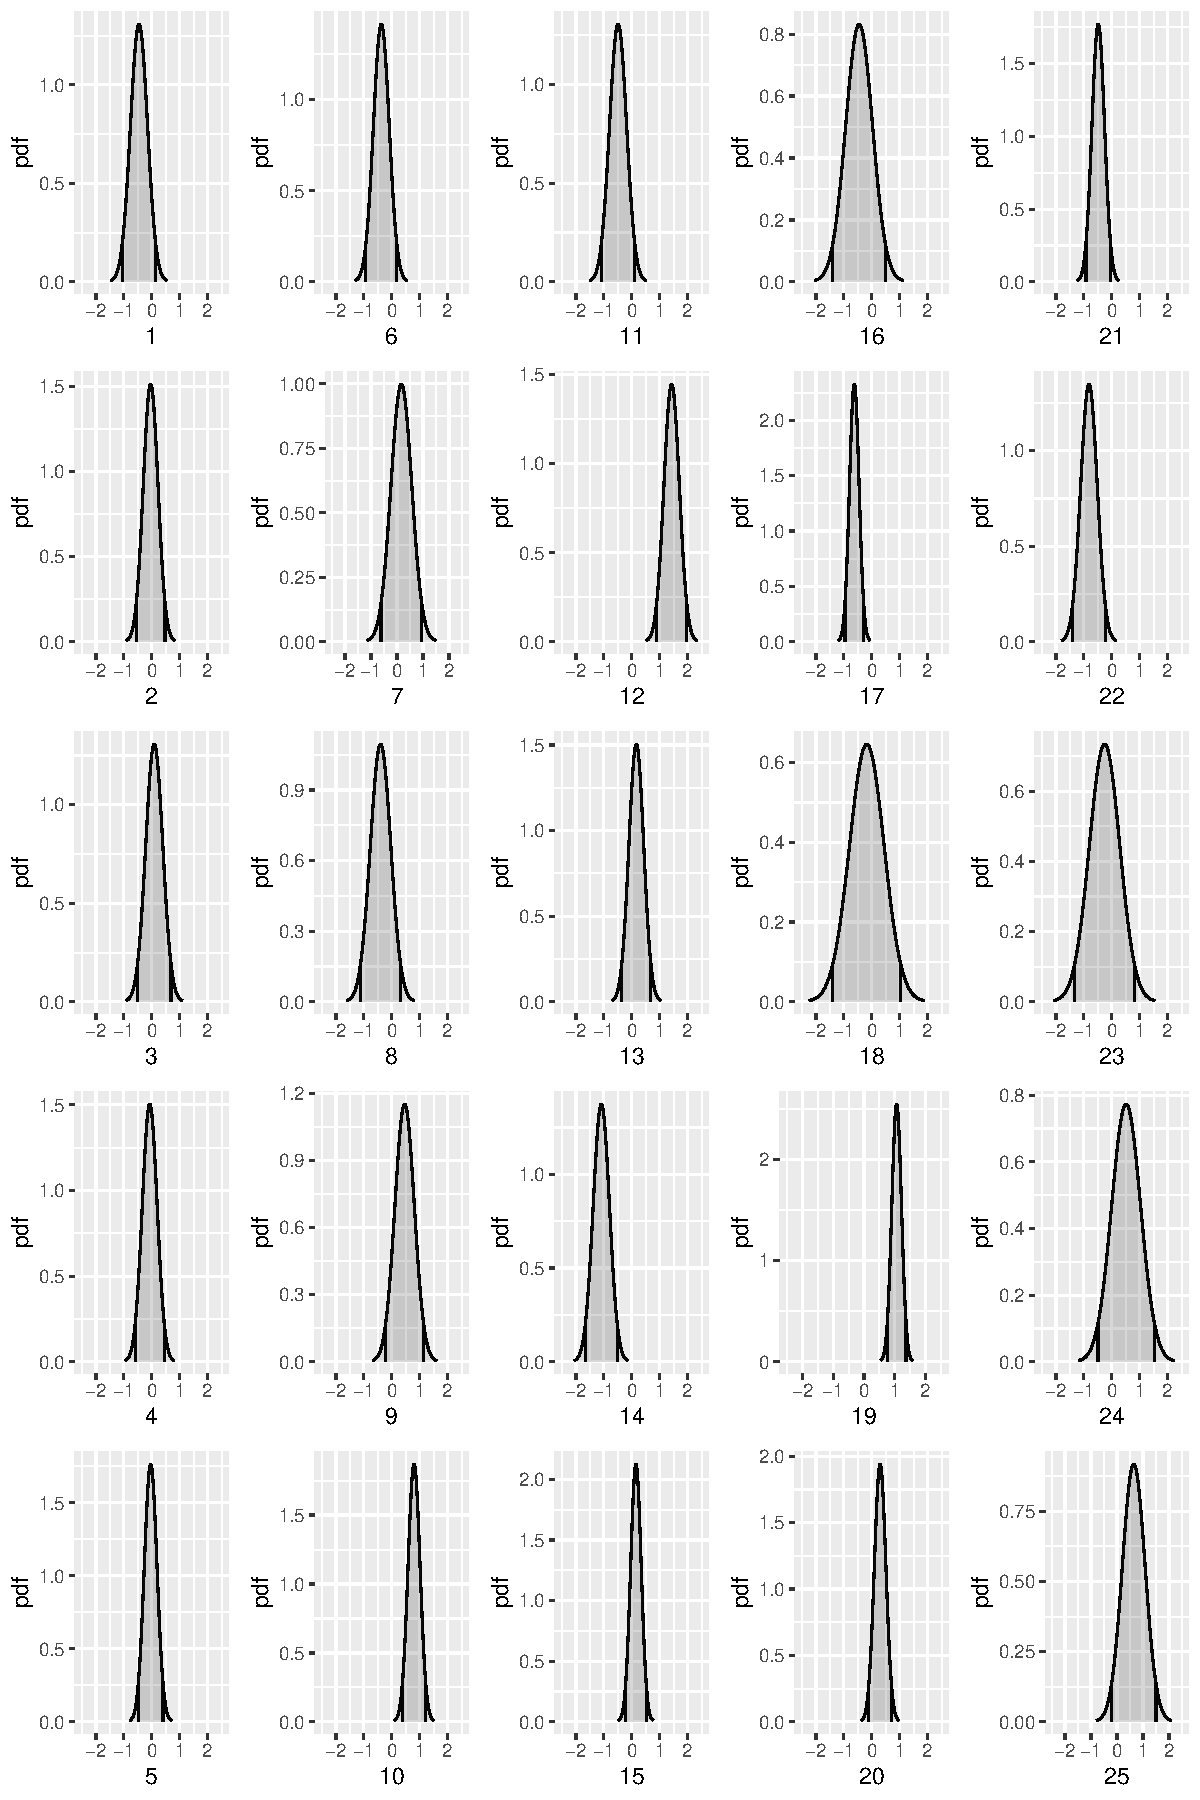
\includegraphics[width = .8\linewidth]{../Plots/scorer_posterior_plot.pdf}
	\caption{\textbf{Posterior estimates of scorer random effects.} Density curves show the posterior estimate along lines indicating the 95\% CI for 25 scorers.}
	\label{fig:scorer_fx}
\end{figure}


\begin{figure}[H]
	\centering
	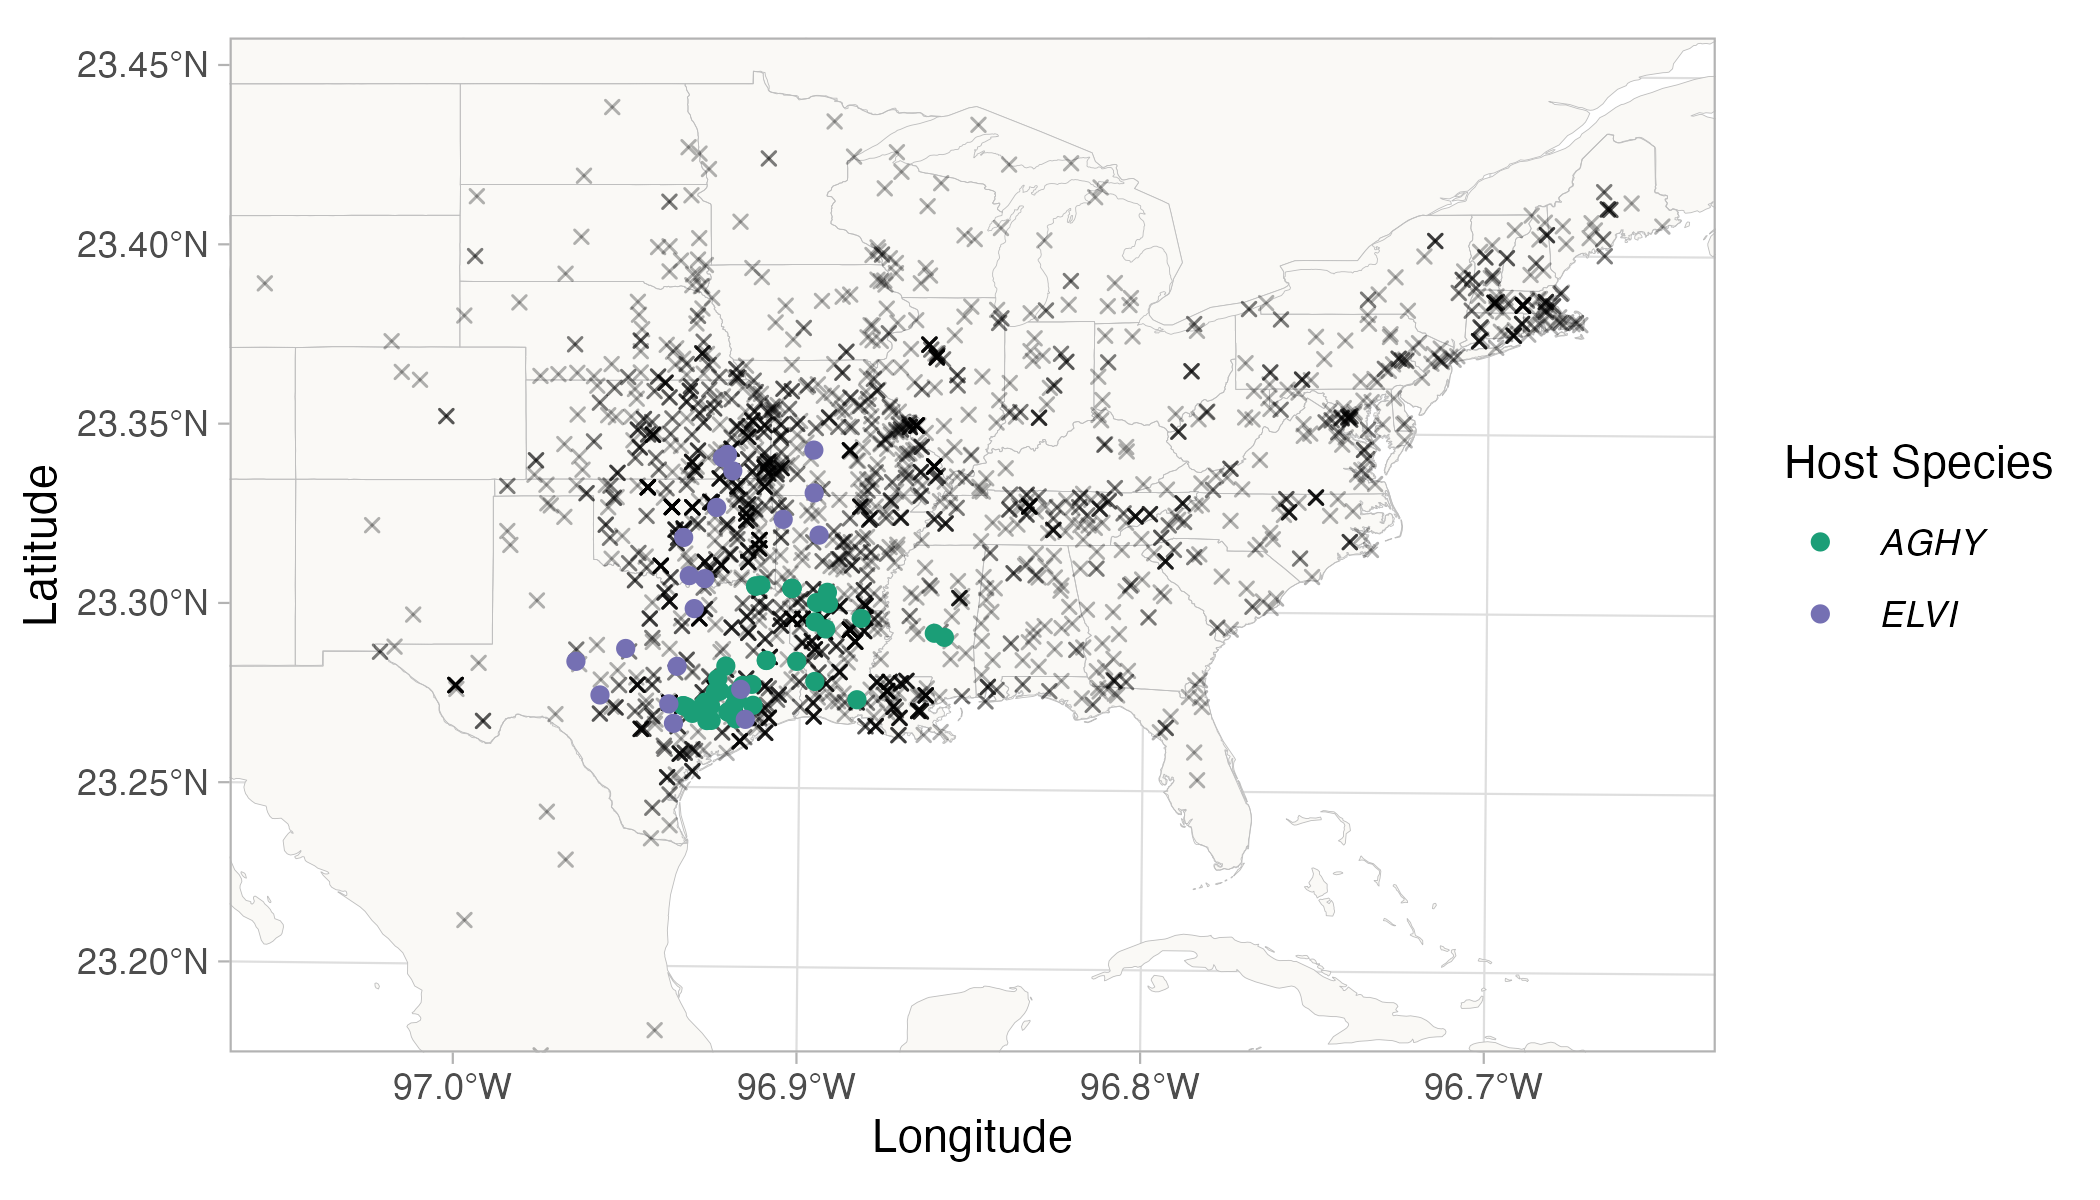
\includegraphics[width = \linewidth]{../Plots/contemp_surveys_map.png}
	\caption{\textbf{Locations of contemporary surveys of endophytes in \emph{A. hyemalis} used as "test" data (red points), relative to the historical collection data (black crosses).}}
	\label{fig:contempsurveysmap}
\end{figure}

	\begin{figure}[H]
	\centering
	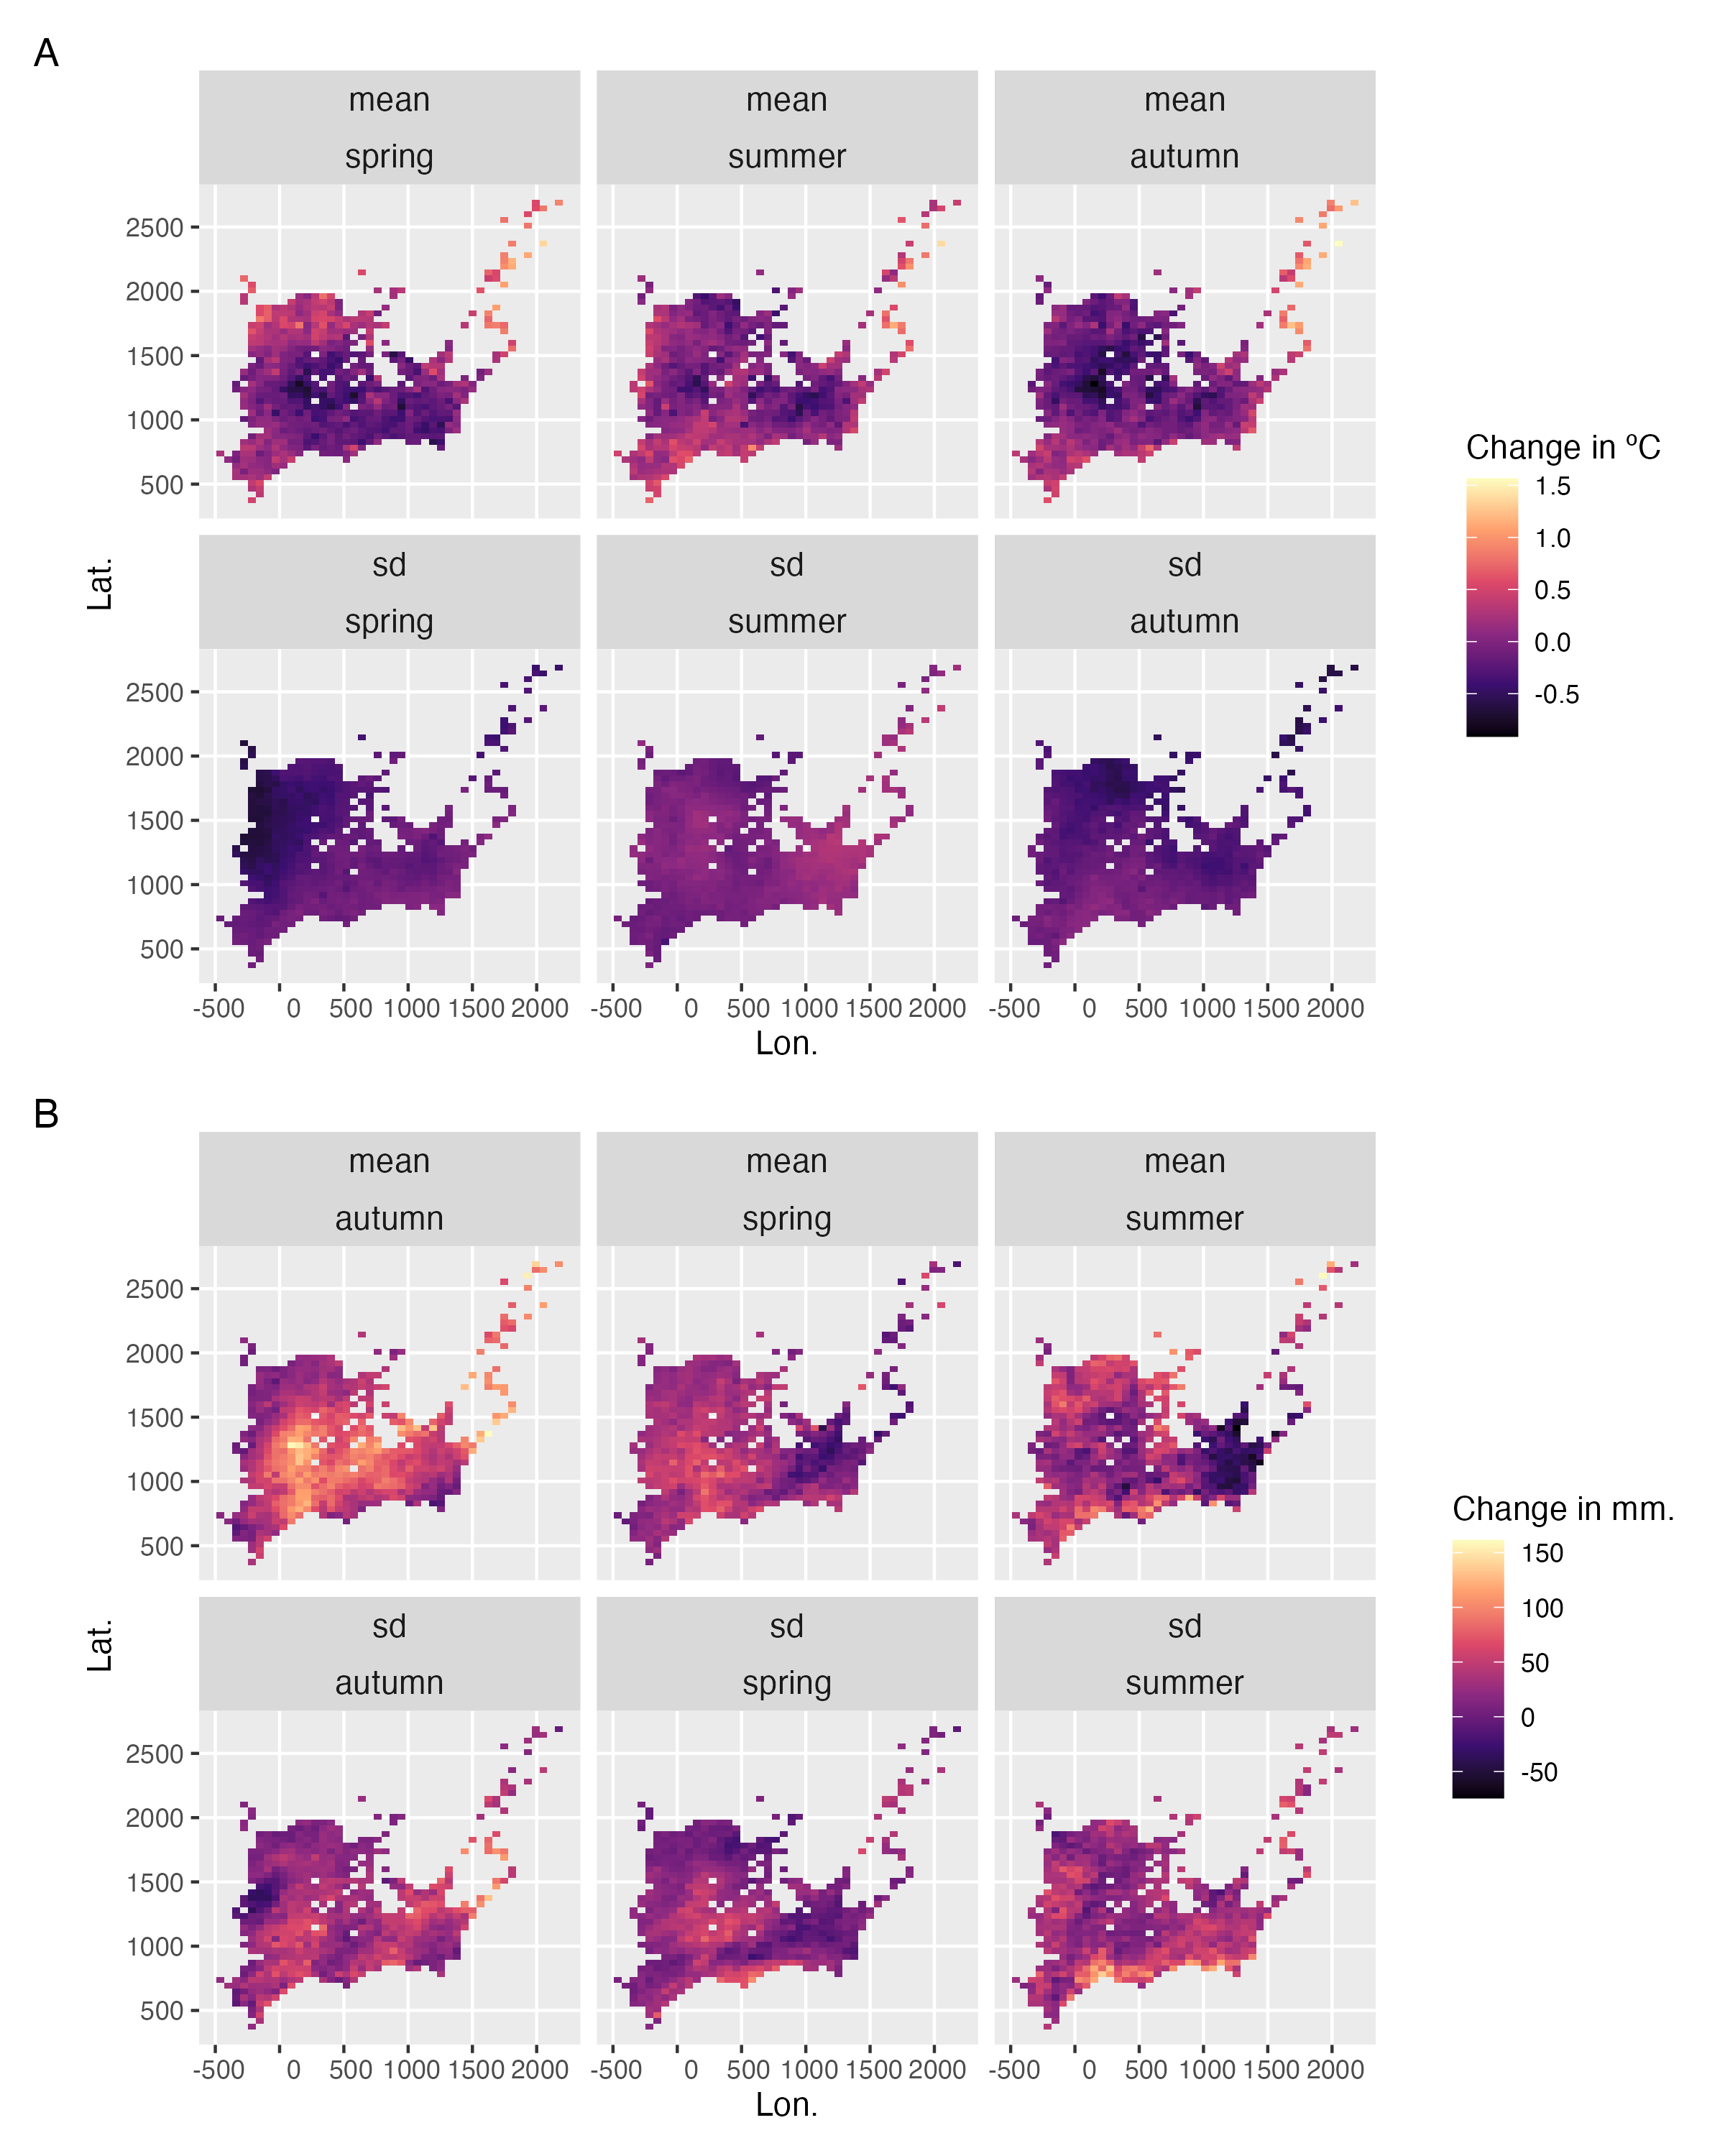
\includegraphics[width = .8\linewidth]{../Plots/AGHY_climate_change_plot.png}
	\caption{\textbf{Change in seasonal climate variables between the periods 1895-1925 and 1990-2020.} Color represents change in (A) seasonal temperature and (B) seasonal precipitation. Maps show pixels covering the modeled distribution of \emph{A. hyemalis} used in post-hoc climate correlation analysis.}
	\label{fig:AGHY_climate_covariates}
\end{figure}

\begin{figure}[H]
	\centering
	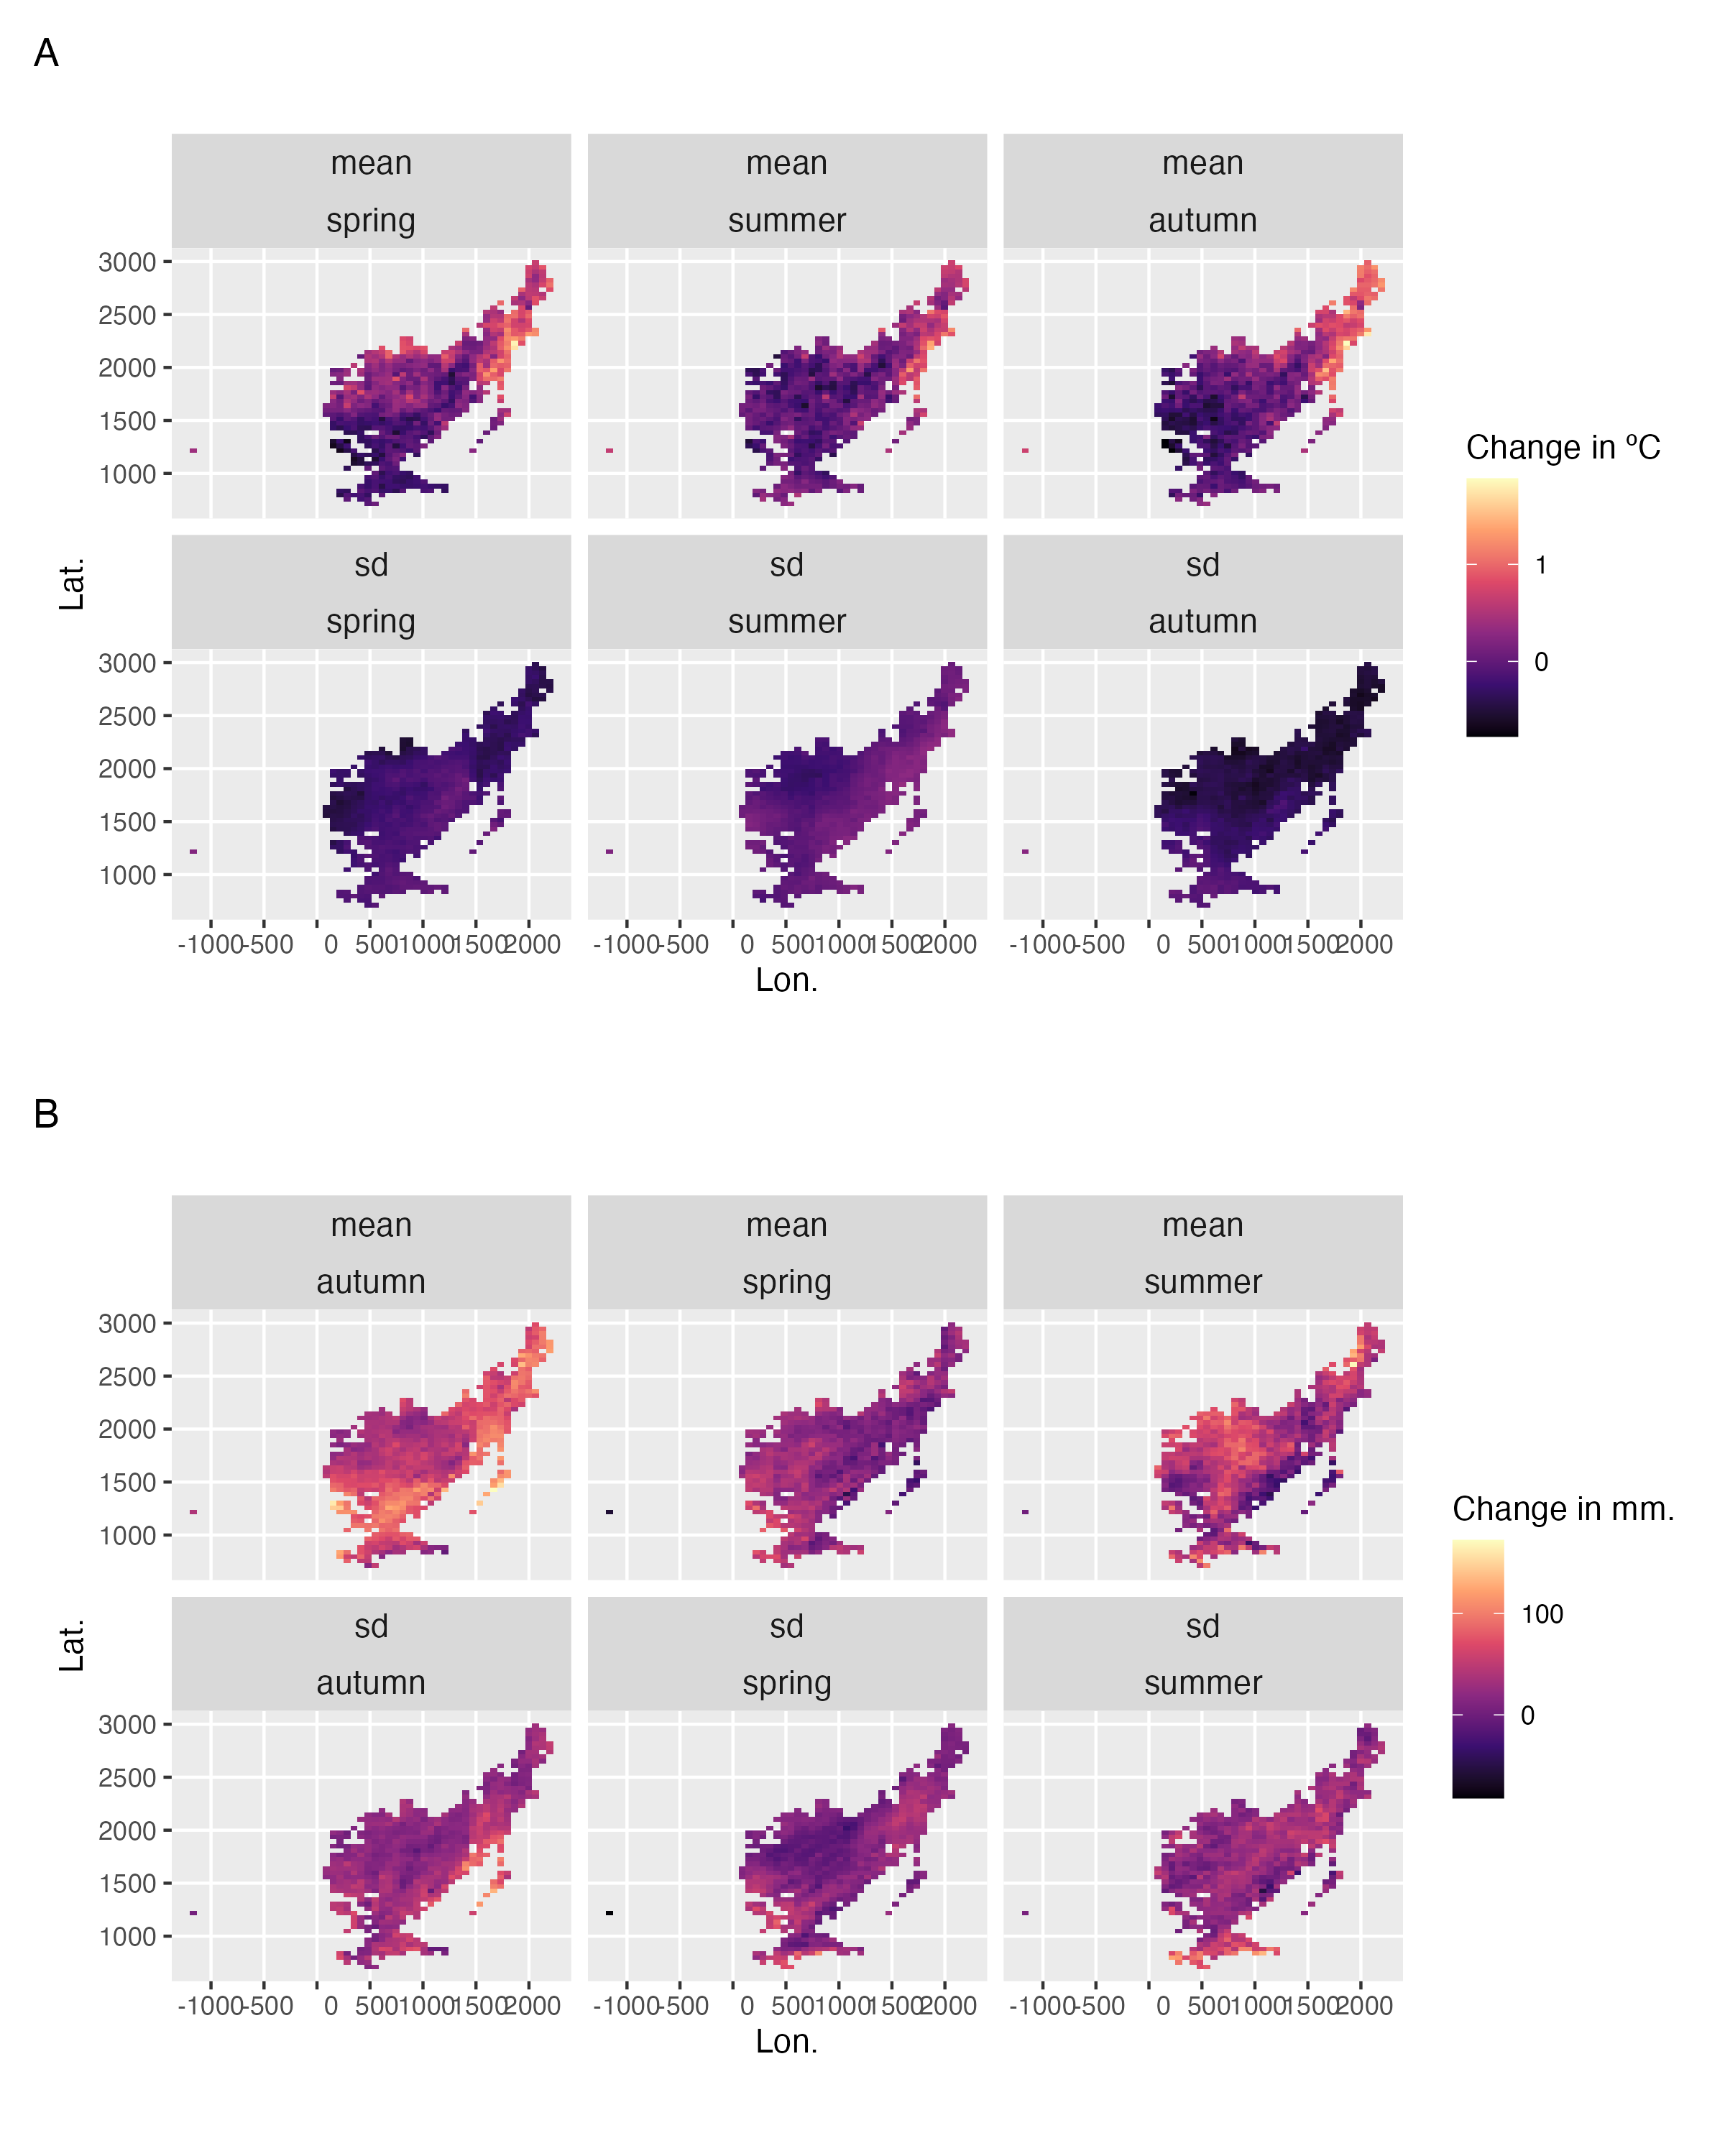
\includegraphics[width = .8\linewidth]{../Plots/AGPE_climate_change_plot.png}
	\caption{\textbf{Change in seasonal climate variables between the periods 1895-1925 and 1990-2020.} Color represents change in (A) seasonal temperature and (B) seasonal precipitation. Maps show pixels covering the modeled distribution of \emph{A. perennans} used in post-hoc climate correlation analysis.}
	\label{fig:AGPE_climate_covariates}
\end{figure}

\begin{figure}[H]
	\centering
	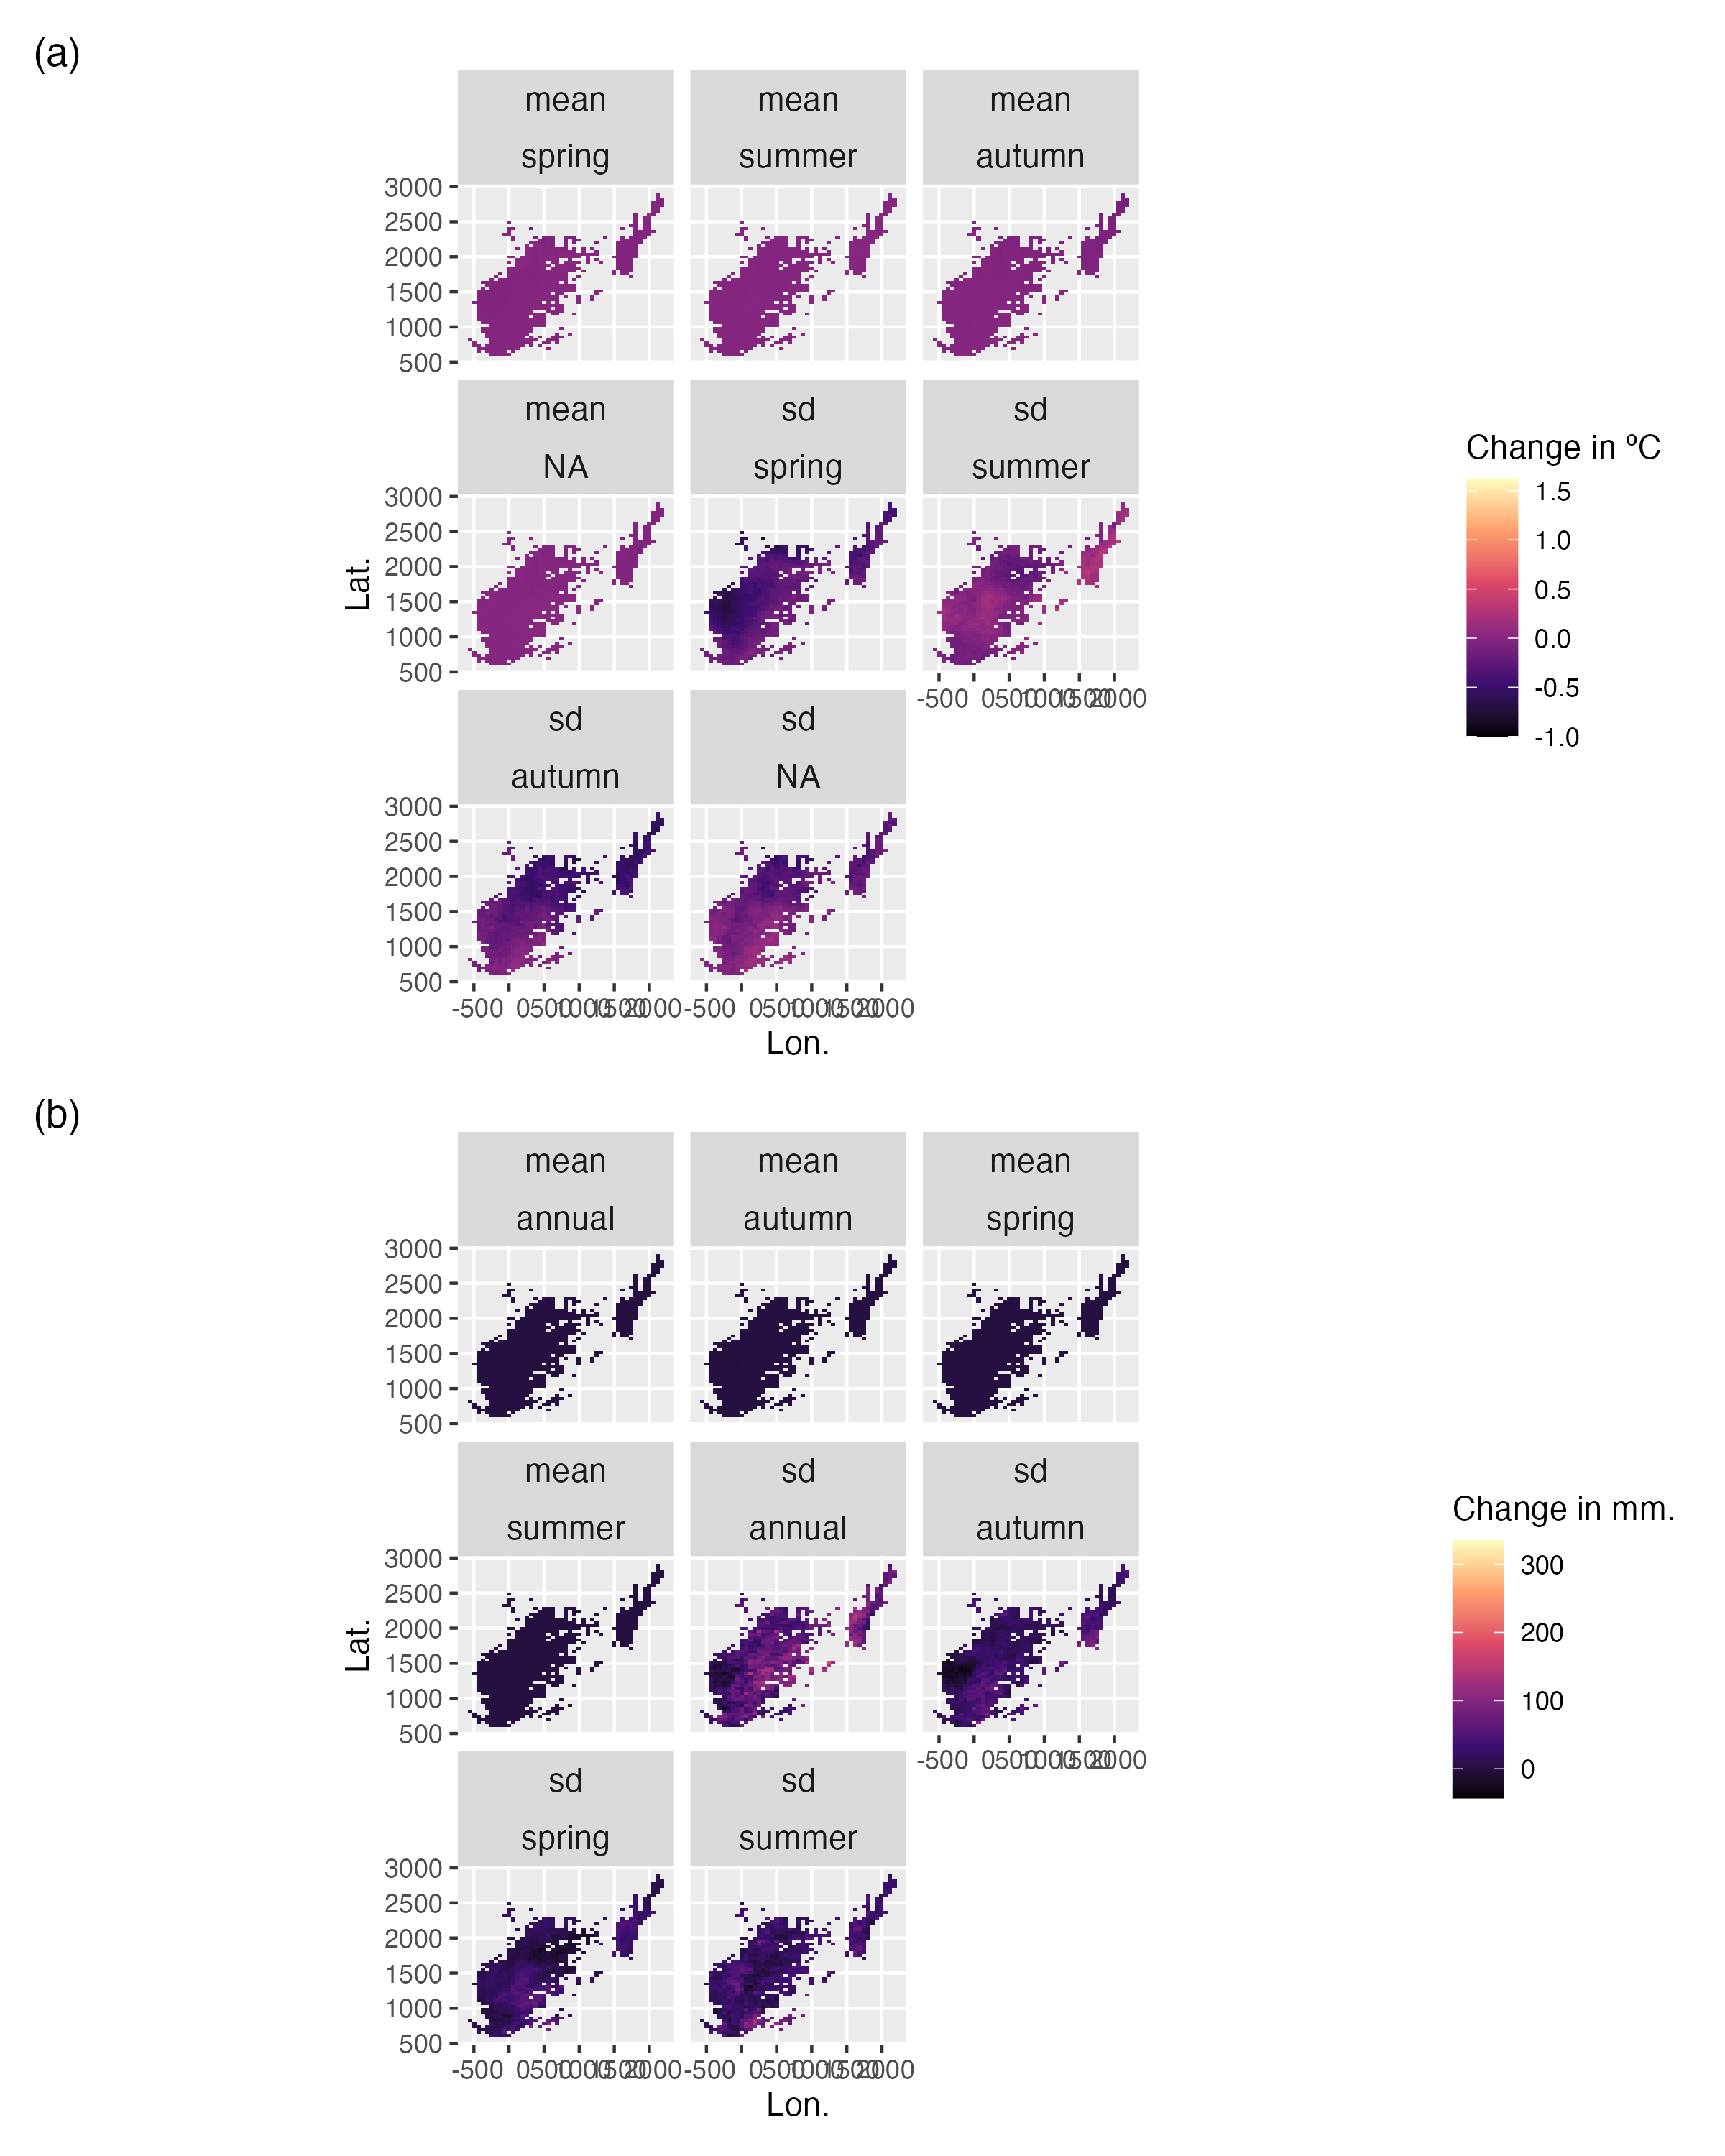
\includegraphics[width = .8\linewidth]{../Plots/ELVI_climate_change_plot.png}
	\caption{\textbf{Change in seasonal climate variables between the periods 1895-1925 and 1990-2020.} Color represents change in (A) seasonal temperature and (B) seasonal precipitation. Maps show pixels covering the modeled distribution of \emph{E. virginicus} used in post-hoc climate correlation analysis.}
	\label{fig:ELVI_climate_covariates}
\end{figure}


	
	\begin{table}[h]
		\caption{Summary of herbarium samples across collections}
		\label{Table:herbaria}
		\centering
		\begin{tabular}{llll}\hline
			Herbarium Collection        & AGHY        & AGPE      &      ELVI\\ \hline
			Botanical Research Institute of Texas &   341   &    189&    176    \\
			Louisiana State University &     71  & --  &   61       \\
			Mercer Botanic Garden &   3    & --     &     6\\
			Missouri Botanic Garden& 78 & 39& 31\\
		    Texas A\&M &  73&-- & 49 \\
		    University of Kansas & 134 & -- &  20\\
		    University of Oklahoma & 65 &30&  91\\
		    University of Texas  \& Lundell   &  169& 41& 99\\		    				 			     			     
			Oklahoma State University&     30  &   --    &  69 \\ \hline
		\end{tabular}
		\bigskip{}

	\end{table}
	
	\section*{Supporting Methods}
	\subsection*{ODMAP Protocol} \label{sec:sdm}
{\color{NavyBlue}{Overview}}\\
\textbf {Model  purpose}: Mapping current distribution of epichloë host species. \\
\textbf {Target species}: \emph{Agrostis hyemalis}, \emph{Agrostis perennans}, and \emph{Elymus virginicus}. \\
\textbf {Study area}: United States \\
%Scale of analysis
\textbf {Spatial extent}: -125.0208, -66.47917, 24.0625, 49.9375 (xmin, xmax, ymin, ymax).\\
\textbf {Spatial resolution}: 0.04166667, 0.04166667 (x, y).\\
\textbf {Temporal extent}: 1990 to 2020.\\
\textbf {Boundary}: Natural.\\
{\color{NavyBlue}{Data}}\\
\textbf {Observation type}: Occurrence records from  Global Biodiversity Information Facility and herbarium collection across the United States. We used 713 occurrences records for \emph{Agrostis hyemalis}, 656 occurrence records for \emph{Agrostis perennans} and 2338 for \emph{Elymus virginicus}.\\
\textbf{Response data type}: occurrence record, presence-only.\\
\textbf{Coordinate reference system}: WGS84 coordinate reference system (EPSG:4326 code)\\
\textbf{Climatic data}:  raster data extracted from PRISM  \\
{\color{NavyBlue}{Model }}\\
\textbf{Model assumption}: We assumed that the target species are at equilibrium with their environment. \\
\textbf{Algorithms}: Maximum entropy (maxent)\\
\textbf{Workflow}: We  described the workflow in the method section of the manuscript. \\
\textbf{Software}:  All statistics were performed using Maxent 3.3.4 and R4.3.1 with packages terra, usdm, spThin and dismo.\\
\textbf{Code availability}: Will  available upon  acceptance\\
\textbf{Data availability}: Will  available upon  acceptance\\
{\color{NavyBlue}{Assessment}}\\
We used AUC to test model performance.\\
{\color{NavyBlue}{Prediction }}\\
We predicted the probability of presence of the host species as a binary maps (presence or absence)

	% In most cases, authors should typeset supplementary material in a separate,
	% author-supplied PDF. For author-supplied PDFs, please consult the
	% AmNat_supp_template.tex document, available from
	% https://www.journals.uchicago.edu/journals/an/instruct 
	%
	% By contrast, the Appendix instructions below apply to cases in which
	% a brief appendix is to appear in print after the main body of the article.
	% That notably includes descriptions of methods, tables defining parameters,
	% and other material necessary for reproducing the MS's results.
	%
	% Please reset counters for the appendix (thus normally figure A1, 
	% figure A2, table A1, etc.).
	%
	% Most AmNat articles have no more than one print appendix. If your article
	% has more than one, counters for each appendix should match the letter of
	% that appendix. For example, tables in Appendix B should be numbered table B1, % table C2, etc. This applies to tables, equations, and figures.
	%
	% It's better not to use the \appendix command, because we have some
	% formatting peculiarities that \appendix conflicts with.
	
	%%%%%%%%%%%%%%%%%%%%%
	% Bibliography
	%%%%%%%%%%%%%%%%%%%%%
	% You can either type your references following the examples below, or
	% compile your BiBTeX database and paste the contents of your .bbl file
	% here. The amnatnat.bst style file should work for this---but please
	% let us know if you run into any hitches with it!
	%
	% If you upload a .bib file with your submission, please upload the .bbl
	% file as well; this will be required for typesetting.
	%
	% The list below includes sample journal articles, book chapters, and
	% Dryad references.
	\newpage{}
\bibliographystyle{plainnat}
\bibliography{endo_herbarium}
	
	\newpage{}
	

	
\end{document}

